\documentclass[aspectratio=169]{beamer}
\usepackage{ctex, hyperref}
\usepackage{calligra}
\usepackage{pifont}
\usepackage{tikz}
\usepackage[T1]{fontenc}
\usepackage{SICNU}

\newtheorem{remark}[theorem]{备注} % 备注环境继承定理的编号
\setbeamertemplate{theorems}[numbered] % 使定理编号
\numberwithin{theorem}{section} % 使定理编号包含章节号
% \usepackage[table]{xcolor}
\usepackage{bm}
\usepackage{subfigure}
\usepackage{ragged2e}
\usepackage{booktabs,makecell, multirow, tabularx}
\usepackage{float}
% \author{图灵的猫}
% \title{THU Beamer Theme}
% \subtitle{毕业设计开题报告}
% \institute{四川师范大学偏微分方程与物理团队}
\title[空间分数阶非线性薛定谔波动方程保结构算法研究
]{空间分数阶非线性薛定谔波动方程保结构算法研究}
\author[刘洋]{\footnotesize 汇报人:刘洋 \quad 导师:冉茂华 副教授}
\institute[四川师范大学偏微分方程与物理团队]{\footnotesize 四川师范大学偏微分方程与物理团队}
\date{\footnotesize \vskip -10pt \today}
\date{2024年5月20日}
\usefonttheme[onlymath]{serif}%修改公式字体
\begin{document}

\kaishu
\begin{frame}
	\titlepage
	\vspace{-2mm}
	\begin{figure}[htpb]
		\begin{center}
			
\includegraphics[width=0.45\linewidth]{pic/SICNU_Logo2.png}
		\end{center}
	\end{figure}
\end{frame}
\begin{frame}
\tableofcontents[sectionstyle=show,subsectionstyle=show/shaded/hide,subsubsectionstyle=show/shaded/hide]
\end{frame}

\section{研究背景}
% \begin{frame}{选题来源和论文类型}
% 	\begin{block}{非线性分数阶薛定谔波动方程(NFSWEs)}
% 		本课题主要考虑具有周期边界条件的 NFSWEs:
% 		\begin{equation}
% 			\left\{\begin{array}{l}
% 				u_{t t}+(-\Delta)^{\alpha / 2} u+\mathrm{i} \kappa u_t+\beta|u|^2 u=0,(\boldsymbol{x}, t) \in \mathbb{R}^d \times(0, T] \\
% 				u(\boldsymbol{x}, 0)=u_0(\boldsymbol{x}), u_t(\boldsymbol{x}, 0)=u_1(\boldsymbol{x}), \boldsymbol{x} \in \mathbb{R}^d
% 				\end{array}\right.\tag{8}
% 		\end{equation}
% 	  \end{block}

% 	  \begin{columns}
% 		\begin{column}{0.45\textwidth}
% 		  \begin{block}{选题来源}
% 			本研究为自选项目,选题源于分数阶微积分和非线性方程数值解法.
% 		  \end{block}
% 		\end{column}
% 		\begin{column}{0.45\textwidth}
% 		  \begin{block}{论文类型}
% 			本研究属于数值计算方向,是理论与实践相结合的应用型研究.	
% 		  \end{block}
% 		\end{column}
% 	  \end{columns}

% \end{frame}

\begin{frame}{NFSWEs和守恒定律}
	\begin{block}{非线性分数阶薛定谔波动方程(NFSWEs)}
		本课题主要考虑具有周期边界条件的 NFSWEs:
		\begin{equation}
			\left\{\begin{array}{l}
				u_{t t}+(-\Delta)^{\alpha / 2} u+\mathrm{i} \kappa u_t+\beta|u|^2 u=0,(\boldsymbol{x}, t) \in \mathbb{R}^d \times(0, T] \\
				u(\boldsymbol{x}, 0)=u_0(\boldsymbol{x}), u_t(\boldsymbol{x}, 0)=u_1(\boldsymbol{x}), \boldsymbol{x} \in \mathbb{R}^d
				\end{array}\right.
		\end{equation}
		\vspace{-5mm}
		\begin{itemize}
		\item 质量守恒律
		\begin{equation}
			G(t)=\kappa\|u(\cdot, t)\|^2+2 \operatorname{Im}\left(u_t, u\right)
		\end{equation}
		\item 能量守恒律
		\begin{equation}\label{eq:10}
			E(t)=\left\|u_t(\cdot, t)\right\|^2+\left\|(-\Delta)^{\frac{\alpha}{4}} u(\cdot, t)\right\|^2+\frac{\beta}{2}\|u(\cdot, t)\|_{L^4}^4
		\end{equation}
	\end{itemize}
	  \end{block}
\end{frame}

\begin{frame}{研究意义}
	\begin{block}{非线性分数阶薛定谔波动方程(NFSWEs)}
		本课题主要考虑具有周期边界条件的 NFSWEs:
		\begin{equation}
			\left\{\begin{array}{l}
				u_{t t}+(-\Delta)^{\alpha / 2} u+\mathrm{i} \kappa u_t+\beta|u|^2 u=0,(\boldsymbol{x}, t) \in \mathbb{R}^d \times(0, T] \\
				u(\boldsymbol{x}, 0)=u_0(\boldsymbol{x}), u_t(\boldsymbol{x}, 0)=u_1(\boldsymbol{x}), \boldsymbol{x} \in \mathbb{R}^d
				\end{array}\right.\tag{1}
		\end{equation}
	  \end{block}

\begin{columns}
\begin{column}{0.45\textwidth}
	\begin{block}{研究价值}
	\begin{itemize}
		\setlength{\itemsep}{6pt}
		\item NFSWEs 应用背景
		\item 哈密顿结构
		\item 保结构算法
		\end{itemize}
	\end{block}
\end{column}
\begin{column}{0.45\textwidth}
	\begin{block}{研究难点}
	\begin{itemize}
		\setlength{\itemsep}{6pt}
		\item 非线性方程
		\item 波算子 $u_{tt} $
		\item 分数阶算子 $(-\Delta)^{\alpha / 2} u $
		\end{itemize}
	\end{block}
\end{column}
\end{columns}

\end{frame}

\section{研究现状}

\begin{frame}{国内外现状分析}
\begin{exampleblock}{\footnotesize \cite{ranLinearlyImplicitConservative2016} \ M. Ran, C. Zhang, A linearly implicit conservative scheme for the fractional nonlinear Schrödinger equation with wave operator, Int J Comput Math. 93 {\color{purple}{(2016)}} 1103–1118.}
\footnotesize
% \vspace{-5mm}
\begin{itemize}
\item 空间方向:
\begin{equation*}
	\Delta_h^\gamma u_j^n=\frac{1}{h^\gamma} \sum_{k=1}^{M-1} g_{j-k}^{(\gamma)} u_k^n, \quad 1 \leq j \leq M-1
\end{equation*}
\item 时间方向:
\begin{equation*}
	\begin{gathered}
		\hat{v}_j^n=\frac{v_j^{n+1}+v_j^{n-1}}{2}, \quad \delta_t v_j^n=\frac{v_j^{n+1}-v_j^n}{\tau} \\
		\delta_{\hat{t}} v_j^n=\frac{v_j^{n+1}-v_j^{n-1}}{2 \tau}, \quad \delta_t^2 v_j^n=\frac{v_j^{n+1}-2 v_j^n+v_j^{n-1}}{\tau^2}
		\end{gathered}
\end{equation*}
\end{itemize}
\begin{columns}
\column{0.15\textwidth}
\begin{block}{\footnotesize 1 维}
\end{block}
\column{0.15\textwidth}
\begin{block}{\footnotesize 空间 2 阶}
\end{block}
\column{0.15\textwidth}
\begin{block}{\footnotesize 时间 2 阶}
\end{block}
\column{0.15\textwidth}
\begin{block}{\footnotesize 能量守恒\ \ding{51}}
\end{block}
\column{0.15\textwidth}
\begin{block}{\footnotesize 质量守恒\ \ding{51}}
\end{block}
\end{columns}

\end{exampleblock}
\end{frame}


	\begin{frame}{国内外现状分析}
		\begin{exampleblock}{\footnotesize \cite{liFastEnergyConserving2018} \ M. Li, Y.-L. Zhao, A fast energy conserving finite element method for the nonlinear fractional Schrödinger equation with wave operator, Appl Math Comput. 338 {\color{purple}{(2018)}} 758–773.}
			\footnotesize
			% \vspace{-5mm}
			\begin{itemize}
			\item 空间方向:
			\begin{equation*}
				\left(\delta_t^2 U^n, v_h\right)+B\left(\tilde{U}^n, v_h\right)+i \kappa\left(\delta_{\hat{t}} U^n, v_h\right)+\frac{\beta}{2}\left(\left(\left|U^{n+1}\right|^2+\left|U^{n-1}\right|^2\right) \tilde{U}^n, v_h\right)=0
			\end{equation*}
			\item 时间方向:
			\begin{equation*}
				\begin{aligned}
					\delta_t^2 v^n & =\frac{v^{n+1}-2 v^n+v^{n-1}}{\tau^2}, \quad \delta_t v^n=\frac{v^{n+1}-v^n}{\tau} \\
					\tilde{v}^n & =\frac{v^{n+1}+v^{n-1}}{2}, \quad \delta_{\hat{t}} v^n=\frac{v^{n+1}-v^{n-1}}{2 \tau}
					\end{aligned}
			\end{equation*}
		\end{itemize}
		\begin{columns}
			\column{0.15\textwidth}
			\begin{block}{\footnotesize 1 维}
			\end{block}
			\column{0.15\textwidth}
			\begin{block}{\footnotesize 空间 2 阶}
			\end{block}
			\column{0.15\textwidth}
			\begin{block}{\footnotesize 时间 2 阶}
			\end{block}
			\column{0.15\textwidth}
			\begin{block}{\footnotesize 能量守恒\ \ding{51}}
			\end{block}
			\column{0.15\textwidth}
			\begin{block}{\footnotesize 质量守恒\ \ding{51}}
			\end{block}
			\end{columns}
	
		\end{exampleblock}
		\end{frame}
				
	
\begin{frame}{国内外现状分析}
	\begin{exampleblock}{\footnotesize \cite{panFourthorderDifferenceScheme2022} \ K. Pan, J. Zeng, D. He, S. Zhang, A fourth-order difference scheme for the fractional nonlinear Schrödinger equation with wave operator, Appl Anal. 101 {\color{purple}{(2020)}} 2886–2902.}
		\footnotesize
		% \vspace{-5mm}
		\begin{itemize}
		\item 空间方向:
		\begin{equation*}
			\begin{gathered}
				\mathcal{A}_h^\alpha f(x)=\frac{\alpha}{24} f(x-h)+\left(1-\frac{\alpha}{12}\right) f(x)+\frac{\alpha}{24} f(x+h) \\
				\Delta_h^\alpha U_j=\mathcal{A}_h^\alpha\left((-\Delta)^{\frac{\alpha}{2}} U_j\right)+O\left(h^4\right) \\
				\mathcal{A}_h^\alpha \delta_t^2 U_j^n+i \mathcal{A}_h^\alpha \delta_{\hat{t}} U_j^n+\Delta_h^\alpha U_j^{\bar{n}}+\mathcal{A}_h^\alpha \beta\left|U_j^n\right|^2 U_j^{\bar{n}}+\mathcal{A}_h^\alpha \omega\left(x_j\right) U_j^{\bar{n}}=0
				\end{gathered}
		\end{equation*}
		\item 时间方向:
		\vspace{-2mm}
		\begin{equation*}
			\begin{gathered}
				P_j^{\bar{n}}=\frac{P_j^{n+1}+P_j^{n-1}}{2}, \quad \delta_t P_j^n=\frac{P_j^{n+1}-P_j^n}{\tau} \\
				\delta_{\hat{t}} P_j^n=\frac{P_j^{n+1}-P_j^{n-1}}{2 \tau}, \quad \delta_t^2 P_j^n=\frac{P_j^{n+1}-2 P_j^n+P_j^{n-1}}{\tau^2}
				\end{gathered}
		\end{equation*}
	\end{itemize}
	\vspace{-3mm}
	\begin{columns}
		\column{0.15\textwidth}
		\begin{block}{\footnotesize 1 维}
		\end{block}
		\column{0.15\textwidth}
		\begin{block}{\footnotesize 空间 4 阶}
		\end{block}
		\column{0.15\textwidth}
		\begin{block}{\footnotesize 时间 2 阶}
		\end{block}
		\column{0.15\textwidth}
		\begin{block}{\footnotesize 能量守恒\ \ding{55}}
		\end{block}
		\column{0.15\textwidth}
		\begin{block}{\footnotesize 质量守恒\ \ding{55}}
		\end{block}
		\end{columns}

	\end{exampleblock}
	\end{frame}


\begin{frame}{国内外现状分析}
	\begin{exampleblock}{\footnotesize \cite{chengConvergenceEnergyconservingScheme2022} \ X. Cheng, H. Qin, J. Zhang, Convergence of an energy-conserving scheme for nonlinear space fractional Schrödinger equations with wave operator, J Comput Appl Math. 400 {\color{purple}{(2022)}} 113762.}
		\footnotesize
		% \vspace{-5mm}
		\begin{itemize}
		\item 空间方向:
		\begin{equation*}
			\delta_x^\alpha v_j^n=-1 /(2 \cos (\alpha \pi / 2))\left(\delta_{x,+}^\alpha v_j^n+\delta_{x,-}^\alpha v_j^n\right)
		\end{equation*}
		\item 时间方向:
		\begin{equation*}
			\begin{aligned}
				& \delta_t U_j^{n+\frac{1}{2}}=V_j^{n+\frac{1}{2}}+R_1^n \\
				& \delta_t V_j^{n+\frac{1}{2}}=\partial_x^\alpha U_j^{n+\frac{1}{2}}-\mathrm{i} V_j^{n+\frac{1}{2}}-B^n W^{n+\frac{1}{2}}+Q_2^n \\
				& \delta_t W^{n+\frac{1}{2}}=\Re\left(B^n, \delta_t U^{n+\frac{1}{2}}\right)+R_3^n
				\end{aligned}
		\end{equation*}
	\end{itemize}
	\begin{columns}
		\column{0.15\textwidth}
		\begin{block}{\footnotesize 2 维}
		\end{block}
		\column{0.15\textwidth}
		\begin{block}{\footnotesize 空间 2 阶}
		\end{block}
		\column{0.15\textwidth}
		\begin{block}{\footnotesize 时间 2 阶}
		\end{block}
		\column{0.15\textwidth}
		\begin{block}{\footnotesize 能量守恒\ \ding{51}}
		\end{block}
		\column{0.15\textwidth}
		\begin{block}{\footnotesize 质量守恒\ \ding{55}}
		\end{block}
		\end{columns}
	
	\end{exampleblock}
	\end{frame}

\begin{frame}{国内外现状分析}
	\begin{exampleblock}{\footnotesize \cite{huEfficientEnergyPreserving2022} \ D. Hu, W. Cai, X.-M. Gu, Y. Wang, Efficient energy preserving Galerkin–Legendre spectral methods for fractional nonlinear Schrödinger equation with wave operator, Appl Numer Math. 172 {\color{purple}{(2022)}} 608–628.}
		\footnotesize
		% \vspace{-5mm}
		\begin{itemize}
		\item 空间方向:
		\begin{equation*}
			\begin{aligned}
				& \mathcal{A}(u, w)=\frac{1}{2 \cos \left(\frac{\pi x}{2}\right)}\left[\left({ }_a^{R L} D_x^{\alpha / 2} u,{ }_x^{R L} D_b^{\alpha / 2} w\right)+\left({ }_x^{R L} D_b^{\alpha / 2} u,{ }_a^{R L} D_x^{\alpha / 2} w\right)\right] \\
				& \left(u_t, w\right)=(v, w) \\
				& \left(v_t, w\right)+\mathcal{A}(u, w)+\mathrm{i} \kappa\left(u_t, w\right)+\beta\left(|u|^2 u, w\right)=0
				\end{aligned}
		\end{equation*}
		\item 时间方向:
		\begin{itemize}
			\item[1.] CN-GLS
			\vspace{-5mm}
		\begin{equation*}
			\begin{aligned}
				u^n & =u\left(x, t_n\right), \quad \delta_t u^{n+\frac{1}{2}}=\frac{u^{n+1}-u^n}{\tau} \\
				u^{n+\frac{1}{2}} & =\frac{u^{n+1}+u^n}{2}, \quad \tilde{u}^{n+\frac{1}{2}}=\frac{3 u^n-u^{n-1}}{2}
				\end{aligned}
		\end{equation*}
	\end{itemize}
\end{itemize}

	
	\end{exampleblock}
	\end{frame}
	
\begin{frame}{国内外现状分析}
	\begin{exampleblock}{\footnotesize \cite{huEfficientEnergyPreserving2022} \ D. Hu, W. Cai, X.-M. Gu, Y. Wang, Efficient energy preserving Galerkin–Legendre spectral methods for fractional nonlinear Schrödinger equation with wave operator, Appl Numer Math. 172 {\color{purple}{(2022)}} 608–628.}
		\footnotesize
		% \vspace{-5mm}
		\begin{itemize}
		\item 时间方向:
		\begin{itemize}
		\item[2.]SAV-GLS
		\vspace{-3mm}
		\begin{equation*}
			p(t)=\sqrt{\int_{\Omega} \frac{1}{2}|u|^4 d x+C_0} \quad \text { with } \quad \mathcal{F}(u)=\frac{|u|^2}{\sqrt{\int_{\Omega} \frac{1}{2}|u|^4 d x+C_0}}
		\end{equation*}
		\item[3.] ESAV-GLS
		\vspace{-3mm}
		\begin{equation*}
			q(t)=\exp \left(\int_{\Omega} \frac{1}{2}|u|^4 d x\right) \quad \text { with } \quad \mathcal{F}(u)=\frac{|u|^2}{\exp \left(\int_{\Omega} \frac{1}{2}|u|^4 d x\right)}
		\end{equation*}
	\end{itemize}
	\end{itemize}
	\vspace{-3mm}
	\begin{columns}
		\column{0.15\textwidth}
		\begin{block}{\footnotesize 1 维}
		\end{block}
		\column{0.15\textwidth}
		\begin{block}{\footnotesize 空间 谱精度}
		\end{block}
		\column{0.15\textwidth}
		\begin{block}{\footnotesize 时间 2 阶}
		\end{block}
		\column{0.15\textwidth}
		\begin{block}{\footnotesize 能量守恒\ \ding{51}}
		\end{block}
		\column{0.15\textwidth}
		\begin{block}{\footnotesize 质量守恒\ \ding{55}}
		\end{block}
		\end{columns}
	
	\end{exampleblock}
	\end{frame}


\begin{frame}{国内外现状分析}
	\begin{exampleblock}{\footnotesize \cite{zhangHighorderStructurepreservingDifference2023} \ X. Zhang, M. Ran, Y. Liu, L. Zhang, A high-order structure-preserving difference scheme for generalized fractional Schrödinger equation with wave operator, Math Comput Simulation. 210 {\color{purple}{(2023)}}  532–546.}
		\footnotesize
		% \vspace{-5mm}
		\begin{itemize}
		\item 空间方向:
		\begin{equation*}
			(-\Delta)^{\alpha / 2} u(x)=\frac{1}{h^\alpha} \sum_{k=-\infty}^{+\infty} \widehat{g}_k^{(\alpha)} u(x-k h)+O\left(h^4\right)
			\end{equation*}
			这里
			\begin{equation*}
			\widehat{g}_k^{(\alpha)}=\left\{\begin{array}{l}
			\frac{4}{3} g_k^{(\alpha)}-\frac{1}{3 \cdot 2^\alpha} g_{\frac{k}{2}}^{(\alpha)}, k \text { is even } \\
			\frac{4}{3} g_k^{(\alpha)}, k \text { is odd }
			\end{array}\right.
			\end{equation*}
			其中
			\begin{equation*}
			g_k^{(\alpha)}=\left(1-\frac{\alpha+1}{\alpha / 2+k}\right) g_{k-1}^{(\alpha)} \text { and } g_0^{(\alpha)}=\frac{\Gamma(\alpha+1)}{\Gamma^2(\alpha / 2+1)}, k=1,2, \ldots
			\end{equation*}
			\end{itemize}
	\end{exampleblock}
	\end{frame}

	\begin{frame}{国内外现状分析}
		\begin{exampleblock}{\footnotesize \cite{zhangHighorderStructurepreservingDifference2023} \ X. Zhang, M. Ran, Y. Liu, L. Zhang, A high-order structure-preserving difference scheme for generalized fractional Schrödinger equation with wave operator, Math Comput Simulation. 210 {\color{purple}{(2023)}}  532–546.}
			\footnotesize
			% \vspace{-5mm}
			\begin{itemize}
			\item 时间方向:
				
			TSAV
		\begin{equation*}
		r(t)=\sin \left(E_1(u)\right)+\varepsilon, \quad \text { where } \quad E_1(u)=\int_{\Omega} F\left(|u|^2\right) d x
		\end{equation*}
		$\mathrm{CN}$ 格式\&外推公式
		\begin{equation*}
		\begin{aligned}
		\delta_t v_j^{n+\frac{1}{2}} & =\frac{v_j^{n+1}-v_j^n}{\tau}, \quad \delta_x v_j^n=\frac{v_{j+1}^n-v_j^n}{h}, \\
		v_j^{n+\frac{1}{2}} & =\frac{v_j^{n+1}+v_j^n}{2}, \quad \tilde{v}_j^{n+\frac{1}{2}}=\frac{3 v_j^n-v_j^{n-1}}{2} .
		\end{aligned}
		\end{equation*}
		\end{itemize}
		\begin{columns}
			\column{0.15\textwidth}
			\begin{block}{\footnotesize 1 维}
			\end{block}
			\column{0.15\textwidth}
			\begin{block}{\footnotesize 空间 4 阶}
			\end{block}
			\column{0.15\textwidth}
			\begin{block}{\footnotesize 时间 2 阶}
			\end{block}
			\column{0.15\textwidth}
			\begin{block}{\footnotesize 能量守恒\ \ding{51}}
			\end{block}
			\column{0.15\textwidth}
			\begin{block}{\footnotesize 质量守恒\ \ding{55}}
			\end{block}
			\end{columns}
		
		\end{exampleblock}
		\end{frame}

\begin{frame}{国内外现状分析}
	% Table generated by Excel2LaTeX from sheet 'Sheet1'
	\begin{table}[htbp]
		\centering
		\small
		\caption{NFSWEs 国内外现状分析}
			\begin{tabular}{lccccc}
			\toprule
			\textcolor[rgb]{0.227,0.373,0.306}{\textbf{文献}} & \textcolor[rgb]{0.227,0.373,0.306}{\textbf{维度}} & \textcolor[rgb]{0.227,0.373,0.306}{\textbf{空间精度}} & \textcolor[rgb]{0.227,0.373,0.306}{\textbf{时间精度}} & \textcolor[rgb]{0.227,0.373,0.306}{\textbf{能量守恒}} & \textcolor[rgb]{0.227,0.373,0.306}{\textbf{质量守恒}} \\
			\midrule
			\textcolor[rgb]{0.227,0.373,0.306}{\textbf{\cite{ranLinearlyImplicitConservative2016}{2016,Ran}}} & 1 维   & 2 阶   & 2 阶   & 修正能量  & 修正质量 \\
			\midrule
			\textcolor[rgb]{0.227,0.373,0.306}{\textbf{\cite{liFastEnergyConserving2018}{2018,Li}}} & 1 维   & 2 阶   & 2 阶   & 修正能量  & 修正质量 \\
			\midrule
			\textcolor[rgb]{0.227,0.373,0.306}{\textbf{\cite{panFourthorderDifferenceScheme2022}{2022,Pan}}} & 1 维   & 4 阶   & 2 阶   & 无     & 无 \\
			\midrule
			\textcolor[rgb]{0.227,0.373,0.306}{\textbf{\cite{chengConvergenceEnergyconservingScheme2022}{2022,Cheng}}} & 2 维   & 2 阶   & 2 阶   & 修正能量  & 无 \\
			\midrule
			\textcolor[rgb]{0.227,0.373,0.306}{\textbf{\cite{huEfficientEnergyPreserving2022}{2022,Hu}}} & 1 维   & 谱精度   & 2 阶   & 修正能量  & 无 \\
			\midrule
			\textcolor[rgb]{0.227,0.373,0.306}{\textbf{\cite{zhangHighorderStructurepreservingDifference2023}{2023,Zhang}}} & 1 维   & 4 阶   & 2 阶   & 修正能量  & 无 \\
			\bottomrule
			\end{tabular}%
		\label{tab:1}%
		\end{table}%
		\end{frame}
	
		\begin{frame}{国内外现状分析}
			% Table generated by Excel2LaTeX from sheet 'Sheet1'
			\begin{table}[htbp]
				\centering
				\small
				\caption{NFSWEs 国内外现状分析}
					\begin{tabular}{lccccc}
					\toprule
					\textcolor[rgb]{0.227,0.373,0.306}{\textbf{文献}} & \textcolor[rgb]{0.227,0.373,0.306}{\textbf{维度}} & \textcolor[rgb]{0.227,0.373,0.306}{\textbf{空间精度}} & \textcolor[rgb]{0.227,0.373,0.306}{\textbf{时间精度}} & \textcolor[rgb]{0.227,0.373,0.306}{\textbf{能量守恒}} & \textcolor[rgb]{0.227,0.373,0.306}{\textbf{质量守恒}} \\
					\midrule
					\textcolor[rgb]{0.227,0.373,0.306}{\textbf{\cite{ranLinearlyImplicitConservative2016}{2016,Ran}}} & 1 维   & 2 阶   & \textcolor{purple}{2 阶}   & \textcolor{purple}{修正能量}  & \textcolor{purple}{修正质量} \\
					\midrule
					\textcolor[rgb]{0.227,0.373,0.306}{\textbf{\cite{liFastEnergyConserving2018}{2018,Li}}} & 1 维   & 2 阶   & \textcolor{purple}{2 阶}   & \textcolor{purple}{修正能量}  & \textcolor{purple}{修正质量} \\
					\midrule
					\textcolor[rgb]{0.227,0.373,0.306}{\textbf{\cite{panFourthorderDifferenceScheme2022}{2022,Pan}}} & 1 维   & \textcolor{purple}{4 阶}   & \textcolor{purple}{2 阶}   & 无     & 无 \\
					\midrule
					\textcolor[rgb]{0.227,0.373,0.306}{\textbf{\cite{chengConvergenceEnergyconservingScheme2022}{2022,Cheng}}} & \textcolor{purple}{2 维}   & 2 阶   & \textcolor{purple}{2 阶}   & 修正能量  & 无 \\
					\midrule
					\textcolor[rgb]{0.227,0.373,0.306}{\textbf{\cite{huEfficientEnergyPreserving2022}{2022,Hu}}} & 1 维   & \textcolor{purple}{谱精度}   & \textcolor{purple}{2 阶}   & 修正能量  & 无 \\
					\midrule
					\textcolor[rgb]{0.227,0.373,0.306}{\textbf{\cite{zhangHighorderStructurepreservingDifference2023}{2023,Zhang}}} & 1 维   & 4 阶   & \textcolor{purple}{2 阶}   & 修正能量  & 无 \\
					\bottomrule
					\end{tabular}%
				\label{tab:2}%
				\end{table}%
				\end{frame}
	
\section{研究内容}
\subsection{SAV-RRK算法}
\begin{frame}{研究内容及其可行性研究}
	\begin{block}{任意高阶显式保结构数值格式}
		\textbf{\textcolor[rgb]{0.227,0.373,0.306}{研究内容:}}
		
		{\footnotesize 本课题将SAV方法与显式RRK方法结合,为二维NFSWEs构造一类任意高阶显式守恒格式.}
		
		\textbf{\textcolor[rgb]{0.227,0.373,0.306}{可行性分析:}}
		\begin{itemize}
			\item {\footnotesize Ketcheson\cite{ketchesonRelaxationRungeKutta2019}提出了松弛龙格-库塔(RRK)方法,该方法可以为任何二次不变量构建显式的守恒格式.}%随后,RRK 技术被扩展到一般凸不变量 \cite{ranochaRelaxationRungeKutta2020}.}
			\item {\footnotesize 标量辅助变量 (SAV) 方法 \cite{chengConvergenceEnergyconservingScheme2022} 可以通过变量变换将能量\eqref{eq:10}转换为新变量的二次形式.}%不变能量二次方化 (IEQ) 方法 \cite{yangLinearUnconditionallyEnergy2017, yangEfficientLinearSchemes2017}和
			\end{itemize}
	\end{block}
	\end{frame}
	
\begin{frame}\frametitle{NFSWEs的SAV重构}
	通过在\eqref{eq:10} 中的$\frac{\beta}{2}\|u(\cdot, t)\|_{L^{4}}^{4}$ 中添加一个正常数 $C_0$ 来保证能量的正性,即
	\begin{align}\label{eq_SAVRRK:9_1}
		E(t)\overset{\text{def}}{=}\left\|u_{t}(\cdot, t)\right\|^{2}+\left\|(-\Delta)^{\frac{\alpha}{4}} u(\cdot, t)\right\|^{2}+\frac{\beta}{2}\|u(\cdot, t)\|_{L^{4}}^{4} + C_0.
	\end{align}
	在此基础上,考虑引入一个标量辅助变量
	\begin{equation}
		w(t)\overset{\text{def}}{=}\sqrt{H(t)+C_0},
	\end{equation}
	其中$H(t)\overset{\text{def}}{=}\frac{\beta}{2}\|u(\cdot, t)\|_{L^{4}}^{4} .$
\end{frame}

\begin{frame}\frametitle{NFSWEs的SAV重构}
因此,NFSWEs可以等效地重新表述为
\begin{align}
& u_t=v, \label{eq_SAVRRK:2-2}\\
& v_t=-(-\Delta)^{\alpha / 2} u-\mathrm{i}\kappa v-b(u) w, \label{eq_SAVRRK:2-3}\\
& w_t=\Re\left(b(u), u_t\right),\label{eq_SAVRRK:2-4}
\end{align}
其中
\begin{align}
b(u)\overset{\text{def}}{=}\beta g(|u|^2) u / \sqrt{H(t)+C_0},
\end{align}
初始条件为
\begin{align}\label{eq_SAVRRK:31}
	u(\boldsymbol{x}, 0)=u_{0}(\boldsymbol{x}), \quad v(\boldsymbol{x}, 0)=u_{1}(\boldsymbol{x}), \quad w(0)=\sqrt{\frac{\beta}{2}\|u_{0}\|_{L^{4}}^{4} +C_0}.
\end{align}
\end{frame}


\begin{frame}\frametitle{傅里叶拟谱离散格式}
	对于正整数$M$和正偶数$N_{x}$、$N_{y}$,定义$\tau={T}/{M}$,$h_{x}={L}/{N_{x}}$,$h_{y}={L}/{N_{y}}$.令$\Omega_{h}=\left\{(x_{i}, y_{j}) \mid 0 \leq i \leq N_x-1;0 \leq j \leq N_y-1\right\}$,$\Omega_{\tau}=\left\{t_{m} \mid 0 \leq m \leq M\right\}$,$\Omega_{h}^{\tau}=\Omega_{h} \times \Omega_{\tau}$,其中$t_{m}=m \tau$,$x_{i}=i h_{x}$,$y_{j}=j h_{y}$.
	在任意时刻$t_m$,定义向量形式
	\begin{align}\label{eq_SAVRRK:47}
	&U^m=\left(u_{0,0}^m, \cdots, u_{N_{x}-1,0}^m, u_{0,1}^m, \cdots, u_{N_{x}-1,1}^m, \cdots, u_{0, N_{y}-1}^m, \cdots, u_{N_{x}-1, N_{y}-1}^m\right)^{T},\\
	&V^m=\left(v_{0,0}^m, \cdots, v_{N_{x}-1,0}^m, v_{0,1}^m, \cdots, v_{N_{x}-1,1}^m, \cdots, v_{0, N_{y}-1}^m, \cdots, v_{N_{x}-1, N_{y}-1}^m\right)^{T},\\
	&W^m=w^m.
	\end{align}
	
	对于定义在$\Omega_{h}$上的任意网格函数$u$和$v$,离散内积和相关的离散范数如下
	\begin{align}\label{eq_SAVRRK:48}
	(u, v)=h_{x} h_{y} \sum_{i=0}^{N_{x}-1} \sum_{j=0}^{N_{y}-1} u_{i, j} \bar{v}_{i, j},\quad\|u\|=(u, u)^{\frac{1}{2}},\quad\|u\|_{\infty}=\sup _{\left(x_{i}, y_{j}\right) \in \Omega_{h}}\left|u_{i, j}\right|.
	\end{align}
	
\end{frame}


\begin{frame}\frametitle{傅里叶拟谱离散格式}
	设$\left(x_{i}, y_{j}\right)$为傅里叶插值点,$u_{N}(x, y)$为$u(x, y)$的插值多项式函数,其中
\begin{align}\label{eq_SAVRRK:50}
u_{N}(x, y)=\sum_{k_{1}=-N_{x} / 2}^{N_{x} / 2} \sum_{k_{2}=-N_{y} / 2}^{N_{y} / 2} \tilde{u}_{k_{1}, k_{2}} e^{\mathrm{i}\mu\left( k_{1} (x+L)+k_{2}(y+L)\right)},
\end{align}
这里$\mu={\pi}/{L}$, 系数
\begin{align}\label{eq_SAVRRK:51}
\tilde{u}_{k_{1}, k_{2}}=\frac{1}{N_{x} c_{k_{1}}} \frac{1}{N_{y} c_{k_{2}}} \sum_{l_1=0}^{N_{x}-1} \sum_{l_2=0}^{N_{y}-1} u(x_{l_1}, y_{l_2}) e^{-\mathrm{i}\mu\left( k_{1}(x_{l_1}+L)+k_{2}(y_{l_2}+L)\right)},
\end{align}
% 其中$c_{k_{1}}=1$对于$\left|k_{1}\right|<N_{x}/2$,$c_{k_{2}}=1$对于$\left|k_{2}\right|<N_{y}/2$,$c_{k_{1}}=2$对于$k_{1}=\pm N_{x}/2$,$c_{k_{2}}=2$对于$k_{2}=\pm N_{y}/2$.
其中
\begin{align}c_{k_1} = \begin{cases} 1, & \text{if } |k_1| < \frac{N_x}{2} \\ 2, & \text{if } |k_1| = \frac{N_x}{2} \end{cases} \quad , \quad c_{k_2} = \begin{cases} 1, & \text{if } |k_2| < \frac{N_y}{2} \\ 2, & \text{if } |k_2| = \frac{N_y}{2} \end{cases}.\end{align}

\end{frame}

\begin{frame}\frametitle{傅里叶拟谱离散格式}
	
因此,分数阶拉普拉斯算子 $-(-\Delta)^{\frac{\alpha}{2}} u(x, y)$ 可以通过以下逼近得到:
\begin{align}\label{eq_SAVRRK:52}
-(-\Delta)^{\frac{\alpha}{2}} u_{N}\left(x, y\right)=-\sum\limits_{k_{1}=-N_{x} / 2}^{N_{x} / 2} \sum\limits_{k_{2}=-N_{y} / 2}^{N_{y} / 2}\left|\left(k_{1} \mu\right)^{2}+\left(k_{2} \mu\right)^{2}\right|^{\frac{\alpha}{2}} \tilde{u}_{k_{1}, k_{2}} e^{\mathrm{i}\mu\left( k_{1} (x+L)+k_{2}(y+L)\right)}.
\end{align}
将 \eqref{eq_SAVRRK:51} 插入 \eqref{eq_SAVRRK:52},并考虑在点$(x_i,y_j)$处得到的方程:
\begin{align}
&-(-\Delta)^{\frac{\alpha}{2}} u_{N}\left(x_{i}, y_{j}\right)\nonumber\\
=&\sum\limits_{l_{1}=0}^{N_{x}-1} \sum\limits_{l_{2}=0}^{N_{y}-1}u(x_{l_{1}}, y_{l_{2}})\Big(-\sum\limits_{k_{1}=\frac{-N_{x}}{2}}^{\frac{N_{x}}{2}} \sum\limits_{k_{2}=\frac{-N_{y}}{2}}^{\frac{N_{y}}{2}} \frac{1}{N_{x} c_{k_{1}}} \frac{1}{N_{y} c_{k_{2}}}\left|\mu^{2} \cdot \mathbf{k}^{2}\right|^{\frac{\alpha}{2}} e^{\mathrm{i} \mu\left(k_{1}\left(x_{i}-x_{l_{1}}\right)+k_{2}\left(y_{j}-y_{l_{2}}\right)\right)}\Big)\nonumber\\
=&\left(D^{\alpha}U\right)_{i+j N_{x}},\label{eq_SAVRRK:53}
\end{align}
\end{frame}

\begin{frame}\frametitle{傅里叶拟谱离散格式}
其中$\mu^{2} \cdot \mathbf{k}^{2}=\mu^{2}\left(k_{1}^{2}+k_{2}^{2}\right)$,$D^{\alpha}$ 是具有以下元素的谱对称微分矩阵:
\begin{align}\label{eq_SAVRRK:54}
\left(D^{\alpha}\right)_{i+j N_{x}, l_{1}+l_{2} N_{x}}=-\sum\limits_{k_{1}=-N_{x} / 2}^{N_{x} / 2} \sum\limits_{k_{2}=-N_{y} / 2}^{N_{y} / 2}\frac{1}{N_{x} c_{k_{1}}} \frac{1}{N_{y} c_{k_{2}}}\left|\mu^{2} \cdot \mathbf{k}^{2}\right|^{\frac{\alpha}{2}} e^{\mathrm{i}\mu\left(k_{1}\left(x_{i}-x_{l_{1}}\right)+k_{2}\left(y_{j}-y_{l_{2}}\right)\right)}.
\end{align}
\end{frame}

\begin{frame}\frametitle{傅里叶拟谱离散格式}
将傅里叶拟谱法应用于等效系统 \eqref{eq_SAVRRK:2-2} - \eqref{eq_SAVRRK:2-4},得到空间半离散系统如下:
\begin{align}
& U_t=V, \label{eq_SAVRRK:3-9}\\
& V_t=D^{\alpha} U-\mathrm{i}\kappa V- b(U) \cdot W, \label{eq_SAVRRK:3-10}\\
& W_t=\Re\left(b(U), U_t\right),\label{eq_SAVRRK:3-11}
\end{align}
其中初始条件为$U^0, V^0, W^0$,这里的$\cdot$表示向量之间的点乘.
\end{frame}

\begin{frame}\frametitle{傅里叶拟谱离散格式}

	\begin{theorem}	\label{thm3}
		空间半离散系统 \eqref{eq_SAVRRK:3-9}-\eqref{eq_SAVRRK:3-11} 具有半离散二次能量守恒律
		\begin{equation}
		\frac{dE}{dt}=0, \label{eq_SAVRRK:313a}
		\end{equation}
		其中
		\begin{equation}
		E(U,V,W)\overset{\text{def}}{=}\|V\|^2 + \|D^\frac{\alpha}{2} U\|^2+\left(W\right)^2.\label{eq_SAVRRK:313}
		\end{equation}
		\end{theorem}
		为简洁起见,引入以下符号:
		\begin{equation}
			\begin{aligned}
				\bm{y}&=\left(U,V,W\right)^T,\quad\bm{y}_0=\left(U^0,V^0,W^0\right)^T , \\
				\bm{f}&=(f^1,f^2,f^3)^T\overset{\text{def}}{=}(V,D^{\alpha} U-\mathrm{i}\kappa V-b(U)\cdot W,\Re\left(b(U), U_t\right))^T.
			\end{aligned}
		\end{equation}
	\end{frame}

\begin{frame}\frametitle{显式SAV-RRK格式}

半离散系统\eqref{eq_SAVRRK:3-9}-\eqref{eq_SAVRRK:3-11}可以表示为:
\begin{equation}
\left\{\begin{array}{l}
\bm{y}_t=\bm{f}(\bm{y}),\quad t \in(0, T],\\
\bm{y}(0)=\bm{y}_0.
\end{array}\right.\label{eq_SAVRRK:3-121}
\end{equation}
设$\bm{y}^m$是$\bm{y}\left(t_m\right)$的近似.\eqref{eq_SAVRRK:3-121}的$s$级显式RK格式\cite{hairerRungeKuttaMethods2015}为:
\begin{equation}
\left\{\begin{array}{l}
\bm{Y}_{m i}=\bm{y}^m+\tau \sum\limits_{j=1}^{i-1} a_{i j} \bm{f}_{m j}, \quad i=1, \ldots, s, \\
\bm{y}^{m+1}=\bm{y}^m+\tau \sum\limits_{i=1}^s b_i \bm{f}_{m i},
\end{array}\right.\label{eq_SAVRRK:4-31}
\end{equation}
其中$\bm{f}_{m j}=\bm{f}\left(\bm{Y}_{m j}\right)$,$j=1, \ldots, s$.
\end{frame}

\begin{frame}\frametitle{显式SAV-RRK格式}
	定义矩阵$A$和向量$b$如下:
	\begin{equation}
	\begin{aligned}
	A & =\left(a_{i j}\right)_{s \times s}, \quad a_{i j}=0 \quad \text {对于} \quad j \geq i, \\
	b & =\left(b_1, \cdots, b_s\right)^T,
	\end{aligned}
	\end{equation}
	于是$s$级显式SAV-RK格式可以用Butcher表表示为:
	\begin{equation}
	\begin{array}{c|c}
	c & A \\
	\hline \\
	& b^T
	\end{array}
	\end{equation}
	其中向量$c=(c_1,c_2,\dots,c_s)$满足$c_i=\sum\limits_{j=1}^s a_{i j}$,$i=1, \ldots, s$.
	
\end{frame}

\begin{frame}\frametitle{显式SAV-RRK格式}
	考虑在区间$\left[\hat{t}_m, \hat{t}_{m+1}\right], m \geq 0$上的单步操作,设$\bm{y}_\gamma^m=\left(U^{m}_{\gamma},V^{m}_{\gamma},W^{m}_{\gamma}\right)^T$是$\bm{y}\left(\hat{t}_m\right)$的数值逼近,
	那么对于\eqref{eq_SAVRRK:3-121},$s$级显式SAV-RRK方法定义为:
	\begin{equation}
	\left\{\begin{array}{l}
	\bm{Y}_{m i}=\bm{y}_\gamma^m+\tau \sum\limits_{j=1}^{i-1} a_{i j} \bm{f}_{m j}, \quad i=1, \ldots, s, \\
	\bm{y}_\gamma^{m+1}=\bm{y}_\gamma^m+\gamma_m \tau \sum\limits_{i=1}^s b_i \bm{f}_{m i}.
	\end{array}\right.\label{eq_SAVRRK:4-3}
	\end{equation}
\end{frame}

\begin{frame}\frametitle{显式SAV-RRK格式}
	$s$级RRK方法\eqref{eq_SAVRRK:4-3}可以用Butcher表表示为:
	\begin{equation}
	\begin{array}{c|c}
	c & A \\
	\hline \\
	& \tilde{b}^T
	\end{array}
	\end{equation}
	其中$\tilde{b}=\gamma_m b$,$\gamma_m\neq 0$, 并且满足:
	\begin{equation}
	\left\{\begin{array}{ll}
	E_{\gamma}^{m+1}=E_{\gamma}^{m}, & \text{若} \quad  \sum\limits_{i=1}^s b_i \bm{f}_{m i} \neq 0,\\
	\gamma_m=1, & \text{若} \quad  \sum\limits_{i=1}^s b_i \bm{f}_{m i} =0,
	\end{array}\right.\label{eq_SAVRRK:4-6}
	\end{equation}
	这里
	\begin{align}\label{eq_SAVRRK:4-6b}
	E_{\gamma}^{m}  =\|V_{\gamma}^{m}\|^2+\|D^\frac{\alpha}{2} U_{\gamma}^{m}\|^2+\big(W_{\gamma}^{m}\big)^2.
	\end{align}
	
\end{frame}

\begin{frame}\frametitle{显式SAV-RRK格式}

	显式SAV-RRK方法\eqref{eq_SAVRRK:4-3}的一个显著优势在于可以精确计算参数$\gamma_m$.
	实际上,从\eqref{eq_SAVRRK:4-6}中可知,当$\sum\limits_{i=1}^s b_i \bm{f}_{m i}=0$时,$\gamma_m=1$.当$\sum\limits_{i=1}^s b_i \bm{f}_{m i}\neq 0$时%,通过直接计算,可以得到:
	\begin{align}
	E_{\gamma}^{m+1}  = & \|V_{\gamma}^{m}\|^2+\|D^\frac{\alpha}{2} U_{\gamma}^{m}\|^2+\big(W_{\gamma}^{m}\big)^2 \nonumber\\
	& + \big(V_{\gamma}^{m},\gamma_m\tau\sum\limits_{i=1}^{s}b_if_{mi}^2\big)+\big(\gamma_m\tau\sum\limits_{i=1}^{s}b_if_{mi}^2,V_{\gamma}^{m}\big)\nonumber\\
	&-\big(U_{\gamma}^{m}, D^{\alpha}\big(\gamma_m\tau\sum\limits_{i=1}^{s}b_if_{mi}^1\big)\big)-\big(\gamma_m\tau\sum\limits_{i=1}^{s}b_if_{mi}^1, D^{\alpha} U_{\gamma}^{m}\big)\nonumber\\
	&+2W_{\gamma}^{m}\gamma_m\tau\sum\limits_{i=1}^{s}b_if_{mi}^3+\big(\gamma_m\tau\sum\limits_{i=1}^{s}b_if_{mi}^3\big)^2.\label{eq_SAVRRK:49}
	\end{align}
		
\end{frame}

\begin{frame}\frametitle{显式SAV-RRK格式}
	将其与\eqref{eq_SAVRRK:4-6}结合,得到:
	\begin{align*}
	&\gamma_m\tau\big[\big(V_{\gamma}^{m},\sum\limits_{i=1}^{s}b_if_{mi}^2\big)+\big(\sum\limits_{i=1}^{s}b_if_{mi}^2,V_{\gamma}^{m}\big)-\big(U_{\gamma}^{m},D^{\alpha}\big(\sum\limits_{i=1}^{s}b_if_{mi}^1\big)\big)-\big(\sum\limits_{i=1}^{s}b_if_{mi}^1, D^{\alpha} U_{\gamma}^{m}\big)\\
	&+2W_{\gamma}^{m}\sum\limits_{i=1}^{s}b_if_{mi}^3\big] +\gamma_m^2\tau^2\big[\big\|\sum\limits_{i=1}^{s}b_if_{mi}^2\big\|^2+ \big\|D^\frac{\alpha}{2}\big(\sum\limits_{i=1}^{s}b_if_{mi}^1\big)\big\|^2+\big(\sum\limits_{i=1}^{s}b_if_{mi}^3\big)^2\big]=0,
	\end{align*}
	这是关于$\gamma_m$的二次方程.注意到$\gamma_m\neq 0$,因此可得:
	\begin{equation}\label{eq_SAVRRK:r1}\small
	\gamma_m \!=\! \frac{\big(\!V_{\gamma}^{m},\sum\limits_{i=1}^{s}b_if_{mi}^2\!\big)\!+\!\big(\!\sum\limits_{i=1}^{s}b_if_{mi}^2,V_{\gamma}^{m}\!\big)\!-\!\big(\!U_{\gamma}^{m},D^{\alpha}\big(\sum\limits_{i=1}^{s}b_if_{mi}^1\big)\!\big)\!-\!\big(\!\sum\limits_{i=1}^{s}b_if_{mi}^1, D^{\alpha} U_{\gamma}^{m}\!\big)\!+\!2W_{\gamma}^{m}\sum\limits_{i=1}^{s}b_if_{mi}^3}{-\tau\big[\big\|\sum\limits_{i=1}^{s}b_if_{mi}^2\big\|^2+\big\|D^\frac{\alpha}{2}\big(\sum\limits_{i=1}^{s}b_if_{mi}^1\big)\big\|^2+\big(\sum\limits_{i=1}^{s}b_if_{mi}^3\big)^2\big]} .
	\end{equation}
	这意味着当$\sum\limits_{i=1}^s b_i \bm{f}_{m i}\neq 0$时,$\gamma_m$的值也可以通过式\eqref{eq_SAVRRK:r1}精确计算.

\end{frame}

\begin{frame}\frametitle{显式SAV-RRK格式}
	\begin{theorem}
		设显式SAV-RK方法\eqref{eq_SAVRRK:4-31}的阶数至少为2,则显式SAV-RRK方法\eqref{eq_SAVRRK:4-3}的解满足
		\begin{equation}
		E_{\gamma}^{m+1}=E_{\gamma}^{m}, \label{eq_SAVRRK:4-10}
		\end{equation}
		其中$E_{\gamma}^{m}$由\eqref{eq_SAVRRK:4-6b}定义.
		\end{theorem}
		
		\begin{proof}
		当$\sum\limits_{i=1}^s b_i \bm{f}_{m i}=0$时,根据\eqref{eq_SAVRRK:4-3}中的第二个方程可知, $\bm{y}_\gamma^{m+1}\equiv\bm{y}_\gamma^m$,它自动满足式\eqref{eq_SAVRRK:4-10}.
		对于$\sum\limits_{i=1}^s b_i \bm{f}_{m i}\neq 0$的情况,可从条件\eqref{eq_SAVRRK:4-6}中得到式\eqref{eq_SAVRRK:4-10}.证毕.
		\end{proof}
\end{frame}

\begin{frame}\frametitle{松弛因子的估计}
	因为$\sum\limits_{i=1}^s b_i \bm{f}_{m i} = 0$的情况很简单, 此处仅关注$\sum\limits_{i=1}^s b_i \bm{f}_{m i} \neq 0$的情况,
	令
	\begin{equation}
	\begin{aligned}\label{eq_SAVRRK:sm}
	S_m(\gamma)=&\big\|V_\gamma^m+\gamma \tau \sum\limits_{i=1}^s b_i \bm{f}_{m i}^2\big\|^2 + \big\|D^\frac{\alpha}{2} \big(U_\gamma^m+\gamma \tau \sum\limits_{i=1}^s b_i \bm{f}_{m i}^1\big)\big\|^2\\
	&+\big(W_\gamma^m+\gamma \tau \sum\limits_{i=1}^s b_i \bm{f}_{m i}^3\big)^2-\|V_\gamma^{m}\|^2 - \|D^\frac{\alpha}{2} U_\gamma^{m}\|^2-\big(W_\gamma^{m}\big)^2,
	\end{aligned}
	\end{equation}
	则式\eqref{eq_SAVRRK:4-6}中定义的$\gamma_m$的值恰好是函数$S_m(\gamma)$的非零根.
	此外,对$S_m(\gamma)$有以下结果.
	\begin{lemma}\label{lem_SAVRRK:5_1}
	设显式SAV-RK方法\eqref{eq_SAVRRK:4-31}的阶数为$p$,则有
	\begin{equation}
	S_m(1)=\mathcal{O}(\tau^{p+1}).
	\end{equation}
	\end{lemma}
\end{frame}

\begin{frame}\frametitle{松弛因子的估计}

	根据引理 \ref{lem_SAVRRK:5_1},可以得到关于松弛因子 $\gamma_m$ 的以下估计.

	\begin{theorem}\label{thm_SAVRRK:5_1}
	设显式 SAV-RK 方法 \eqref{eq_SAVRRK:4-31} 的阶数为 $p~(p \geq 2)$,那么在式 \eqref{eq_SAVRRK:4-6} 中定义的松弛因子 $\gamma_m$ 满足
	\begin{equation}\label{eq_SAVRRK:5_3}
	\gamma_m=1+\mathcal{O}(\tau^{p-1}).
	\end{equation}
	\end{theorem}	
	\begin{remark}\label{rk_SAVRRK:5_1}
		定理 \ref{thm_SAVRRK:5_1} 表明,当 $\tau\rightarrow 0$ 时,松弛因子 $\gamma_m$ 接近于 $1$,
		这意味着松弛RK方法可以被视为标准RK方法的小扰动.
		\end{remark}
\end{frame}
\begin{frame}\frametitle{显式SAV-RRK方法的截断误差}

	数值解$\bm{y}_\gamma^{m+1}$在$\hat{t}_{m+1}$处可以用两种方式解释\cite{ketchesonRelaxationRungeKutta2019},即增量方向技术(IDT)和松弛技术(RT).
	\begin{itemize}
	\item[1.] IDT的角度:$\bm{y}_\gamma^{m+1}$被视为对$\bm{y}\left(\hat{t}_m+\tau\right)$的近似,当$m \geq 0$,$\hat{t}_m=t_m$.
	\item[2.] RT的角度:$\bm{y}_\gamma^{m+1}$被视为对$\bm{y}\left(\hat{t}_m+\gamma_m \tau\right)$的近似,当$m>0$时,$\hat{t}_m$可能不等于$t_m$.
	\end{itemize}
	
	值得注意的是, 对数值解$\bm{y}_\gamma^{m+1}$的不同解释可能导致不同的收敛结果.

	\begin{theorem}\label{thm_SAVRRK:5_4}
	设显式SAV-RK方法\eqref{eq_SAVRRK:4-31}的阶数为$p~(p \geq 2)$, 以下结论成立:
	\begin{itemize}
	\item 对于IDT,显式SAV-RRK方法\eqref{eq_SAVRRK:4-3}的阶数为$p-1$.
	\item 对于RT,显式SAV-RRK方法\eqref{eq_SAVRRK:4-3}的阶数为$p$.
	\end{itemize}
	\end{theorem}
\end{frame}

\begin{frame}\frametitle{数值算例}
	不失一般性的,在计算中使用了以下的显式RK方法\cite{shuEfficientImplementationEssentially1988}:
	\begin{enumerate}
	\item $\operatorname{RK}(2,2)$:两级二阶Heun方法%\cite{shuEfficientImplementationEssentially1988}.
	\begin{equation}
	\begin{array}{c|cc}
	0 & 0 & 0 \\
	\frac{2}{3} & \frac{2}{3} & 0 \\
	\hline & \frac{1}{4} & \frac{3}{4}
	\end{array}
	\end{equation}
		
	\item $\mathrm{RK}(3,3)$:三级三阶Heun方法%\cite{shuEfficientImplementationEssentially1988}.
		
	\begin{equation}
	\begin{array}{c|ccc}
	0 & 0 & 0 & 0 \\
	\frac{1}{3} & \frac{1}{3} & 0 & 0 \\
	\frac{2}{3} & 0 & \frac{2}{3} & 0 \\
	\hline & \frac{1}{4} & 0 & \frac{3}{4}
	\end{array}
	\end{equation}
	\end{enumerate}
\end{frame}
\begin{frame}\frametitle{数值算例}
	
	\begin{enumerate}[3]
		\item $\operatorname{RK}(4,4)$:四级四阶Gill方法%\cite{shuEfficientImplementationEssentially1988}.
			
	\begin{equation}
	\begin{array}{c|cccc}
	0 & 0 & 0 & 0 & 0 \\
	\frac{1}{2} & \frac{1}{2} & 0 & 0 & 0 \\
	\frac{1}{2} & \frac{\sqrt{2}-1}{2} & 1-\frac{\sqrt{2}}{2} & 0 & 0 \\
	1 & 0 & -\frac{\sqrt{2}}{2} & 1+\frac{\sqrt{2}}{2} & 0 \\
	\hline & \frac{1}{6} & \frac{2-\sqrt{2}}{6} & \frac{2+\sqrt{2}}{6} & \frac{1}{6}
	\end{array}
	\end{equation}
	\end{enumerate}
\end{frame}

\begin{frame}\frametitle{数值算例}
	鉴于数值算例中能量的固有正性,在计算中简单地设置常数$C_0=0$.

	时间方向上的误差和收敛阶通过以下方式计算:
	\begin{equation}
		\text{Error}(\tau) = \|U_{N}^{M} - U_{N}^{2 M}\|_{\infty},~\text{order} = \log_{2}\left[\frac{\text{Error}(\tau)}{\text{Error}(\tau / 2)}\right].\label{eq_SAVRRK:104}
	\end{equation}
	
	为了展示守恒性能,定义相对能量误差:
	\begin{equation}\label{eq_SAVRRK:105}
		R E_{\gamma}^{m} = \left|\frac{E_{\gamma}^{m} - E_{\gamma}^{0}}{E_{\gamma}^{0}}\right|,
	\end{equation}
	其中$E_{\gamma}^{m}$表示时刻$t_m$处的离散能量.
\end{frame}
\begin{frame}\frametitle{数值算例}
		\begin{example}\label{exp_SAVRRK:1}
			考虑一维NFSWEs,形式如下\cite{ranLinearlyImplicitConservative2016}:
			\begin{equation}\label{eq_SAVRRK:108}
				u_{t t}+(-\Delta)^{\alpha / 2} u+\mathrm{i}u_t+|u|^2 u=0, \quad (x,t)\in  (-25, 25)\times[0, T],
			\end{equation}
			其中 $u(x, 0)=(1+\mathrm{i}) x e^{-10(1-x)^2}$ 且 $u_t(x, 0)=0$.
			\end{example}	
\end{frame}

\begin{frame}%\frametitle{数值算例}

	\begin{table}[H]\scriptsize
		\centering
		\caption{当 $N=32$,$T = 1$ 时,例 \ref{exp_SAVRRK:1} 在时间方向的误差和收敛阶}
		\begin{tabular}{lllllrlrlrlrlrl}
		\toprule
		\multicolumn{2}{l}{\multirow{2}[3]{*}{\textbf{RK(级,阶)}}} & \multicolumn{2}{l}{\multirow{2}[3]{*}{$\bm{\tau}$}} & \multicolumn{3}{c}{\textbf{SAV-RK}} &       & \multicolumn{3}{c}{\textbf{SAV-RRK(RT)}} &       & \multicolumn{3}{c}{\textbf{SAV-RRK(IDT)}} \\
		\cmidrule{5-7}\cmidrule{9-11}\cmidrule{13-15}    \multicolumn{2}{l}{} & \multicolumn{2}{l}{} & \textbf{Error($\tau$)} &       & \textbf{order} &       & \textbf{Error($\tau$)} &       & \textbf{order} &       & \textbf{Error($\tau$)} &       & \textbf{order} \\
		\hline
		\multicolumn{2}{l}{\multirow{5}[0]{*}{\textbf{RK(2,2)}}} & \multicolumn{2}{l}{0.1} & 1.8552E-04 &       & -     &       & 1.9063E-04 &       & -     &       & 2.0325E-04 &       & - \\
		\multicolumn{2}{l}{} & \multicolumn{2}{l}{0.05} & 4.6601E-05 &       & 1.9931  &       & 4.7240E-05 &       & 2.0126  &       & 5.0585E-05 &       & 2.0065  \\
		\multicolumn{2}{l}{} & \multicolumn{2}{l}{0.025} & 1.1671E-05 &       & 1.9974  &       & 1.1750E-05 &       & 2.0074  &       & 1.2387E-05 &       & 2.0298  \\
		\multicolumn{2}{l}{} & \multicolumn{2}{l}{0.0125} & 2.9200E-06 &       & 1.9990  &       & 2.9294E-06 &       & 2.0040  &       & 2.9549E-06 &       & 2.0677  \\
		\multicolumn{2}{l}{} & \multicolumn{2}{l}{0.00625} & 7.3022E-07 &       & 1.9996  &       & 7.3130E-07 &       & 2.0021  &       & 6.6665E-07 &       & 2.1481  \\
		\multicolumn{2}{l}{\multirow{5}[0]{*}{\textbf{RK(3,3)}}} & \multicolumn{2}{l}{0.1} & 7.6862E-06 &       & -     &       & 2.9857E-06 &       & -     &       & 1.7245E-04 &       & - \\
		\multicolumn{2}{l}{} & \multicolumn{2}{l}{0.05} & 9.5269E-07 &       & 3.0122  &       & 3.9037E-07 &       & 2.9352  &       & 4.3389E-05 &       & 1.9907  \\
		\multicolumn{2}{l}{} & \multicolumn{2}{l}{0.025} & 1.1866E-07 &       & 3.0052  &       & 5.0077E-08 &       & 2.9626  &       & 1.0873E-05 &       & 1.9966  \\
		\multicolumn{2}{l}{} & \multicolumn{2}{l}{0.0125} & 1.4809E-08 &       & 3.0023  &       & 6.3449E-09 &       & 2.9805  &       & 2.7208E-06 &       & 1.9986  \\
		\multicolumn{2}{l}{} & \multicolumn{2}{l}{0.00625} & 1.8497E-09 &       & 3.0011  &       & 7.9858E-10 &       & 2.9901  &       & 6.8049E-07 &       & 1.9994  \\
		\multicolumn{2}{l}{\multirow{5}[1]{*}{\textbf{RK(4,4)}}} & \multicolumn{2}{l}{0.1} & 3.7701E-07 &       & -     &       & 3.8894E-07 &       & -     &       & 7.0733E-07 &       & - \\
		\multicolumn{2}{l}{} & \multicolumn{2}{l}{0.05} & 2.3572E-08 &       & 3.9994  &       & 2.3939E-08 &       & 4.0221  &       & 4.4585E-08 &       & 3.9878  \\
		\multicolumn{2}{l}{} & \multicolumn{2}{l}{0.025} & 1.4730E-09 &       & 4.0003  &       & 1.4843E-09 &       & 4.0115  &       & 2.8080E-09 &       & 3.9889  \\
		\multicolumn{2}{l}{} & \multicolumn{2}{l}{0.0125} & 9.2041E-11 &       & 4.0003  &       & 9.2397E-11 &       & 4.0058  &       & 1.7743E-10 &       & 3.9842  \\
		\multicolumn{2}{l}{} & \multicolumn{2}{l}{0.00625} & 5.7518E-12 &       & 4.0002  &       & 5.7630E-12 &       & 4.0029  &       & 1.1309E-11 &       & 3.9718  \\
		\bottomrule
		\end{tabular}%
		\label{tab_SAVRRK:6-1}%
		\end{table}%
\end{frame}

\begin{frame}%\frametitle{数值算例}

\begin{figure}[H]
	\begin{center}
	\subfigure[$\max_m\left|\gamma_m-1\right|$]{ \centering
	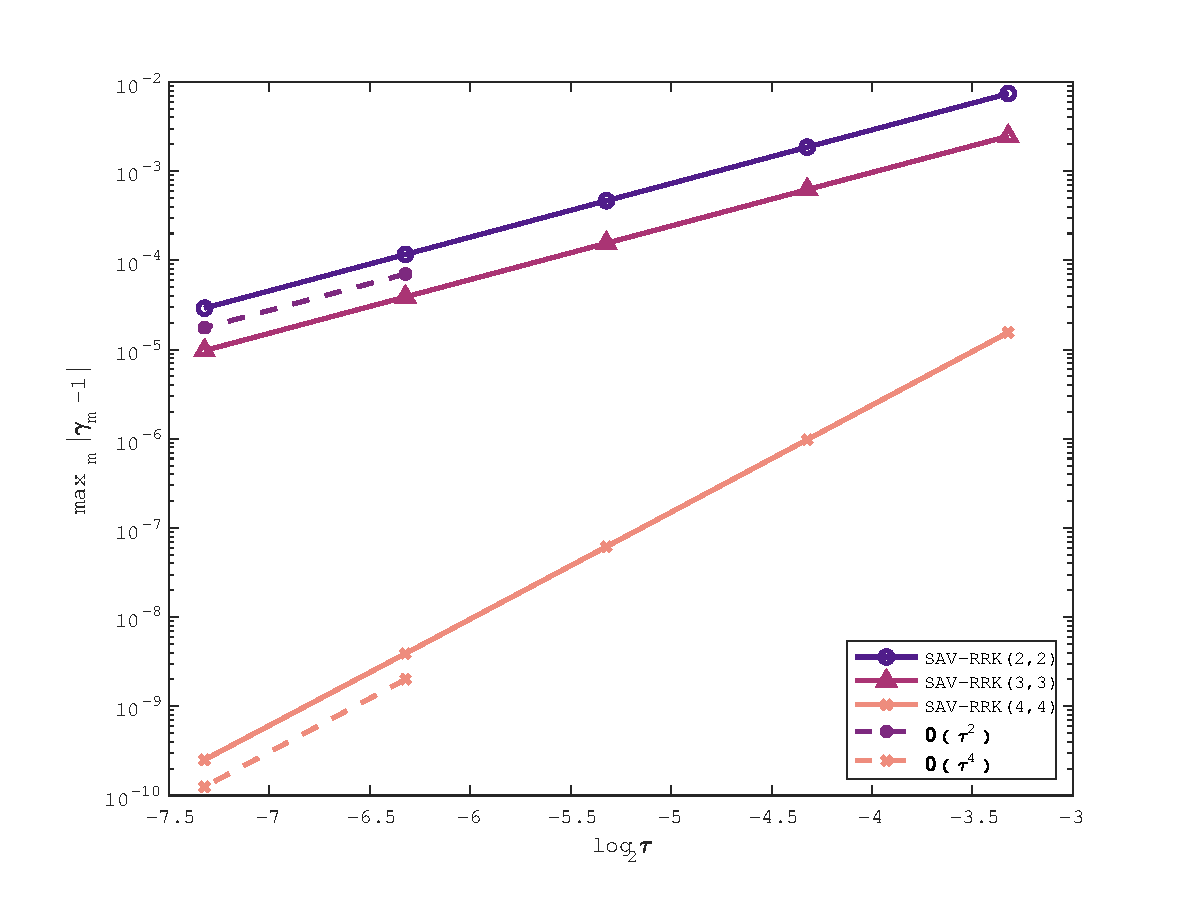
\includegraphics[width=0.5\textwidth]{./figures/exp1_r.eps}
	%\centerline{($b$) Spatial accuracy with $\tau = 10^{-3}.$}
	}\subfigure[$\max_m\left|S_m(1)\right|$]{ \centering
	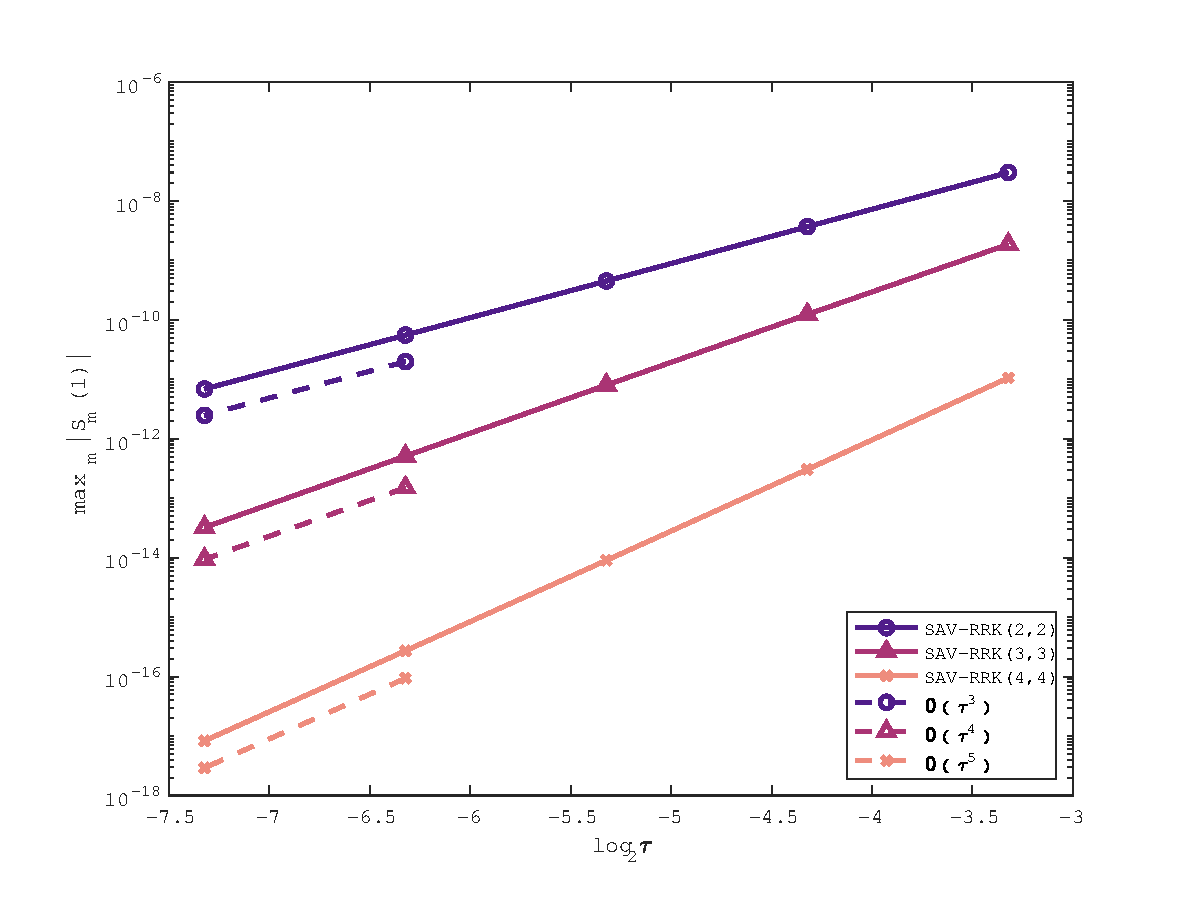
\includegraphics[width=0.5\textwidth]{./figures/exp1_s.eps}
	%\centerline{($a$) Temporal accuracy with $N=128.$}
	}
	% \caption{$\max_m\left|\gamma_m-1\right|$ and $\max_m\left|S_m(1)\right|$ for some relaxation methods in Example \ref{exp_SAVRRK:1}.}
	\caption{例 \ref{exp_SAVRRK:1}中一些松弛格式(RT)所对应的$\max_m\left|\gamma_m-1\right|$ 和 $\max_m\left|S_m(1)\right|$.}
	\label{fig_SAVRRK:1}
	\end{center}
	\end{figure}
\end{frame}
\begin{frame}%\frametitle{数值算例}
	\begin{figure}[H]
		\begin{center}
		\subfigure[$\alpha=1.3$]{ \centering
		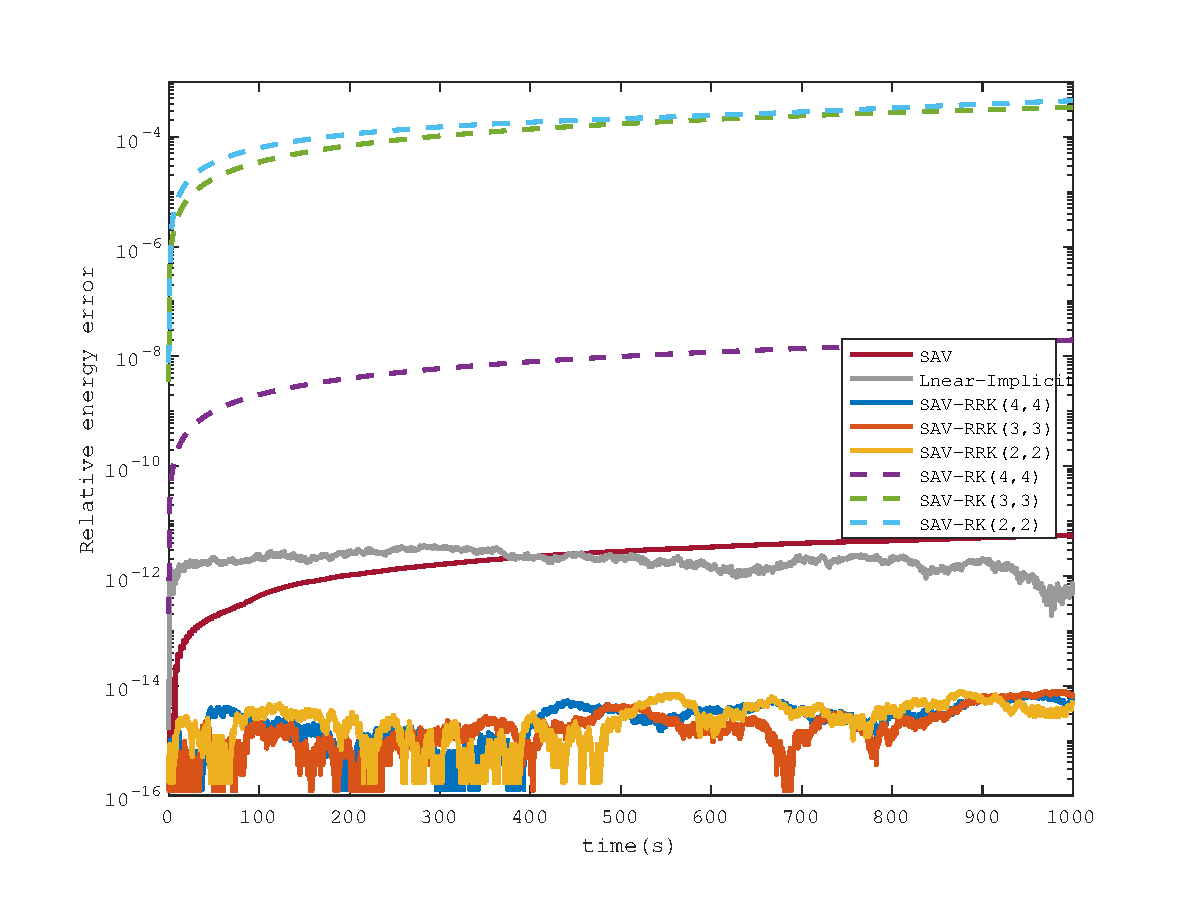
\includegraphics[width=0.5\textwidth]{./figures/exp1_energy3.eps}
		%\centerline{($b$) Spatial accuracy with $\tau = 10^{-3}.$}
		}\subfigure[$\alpha=1.6$]{ \centering
		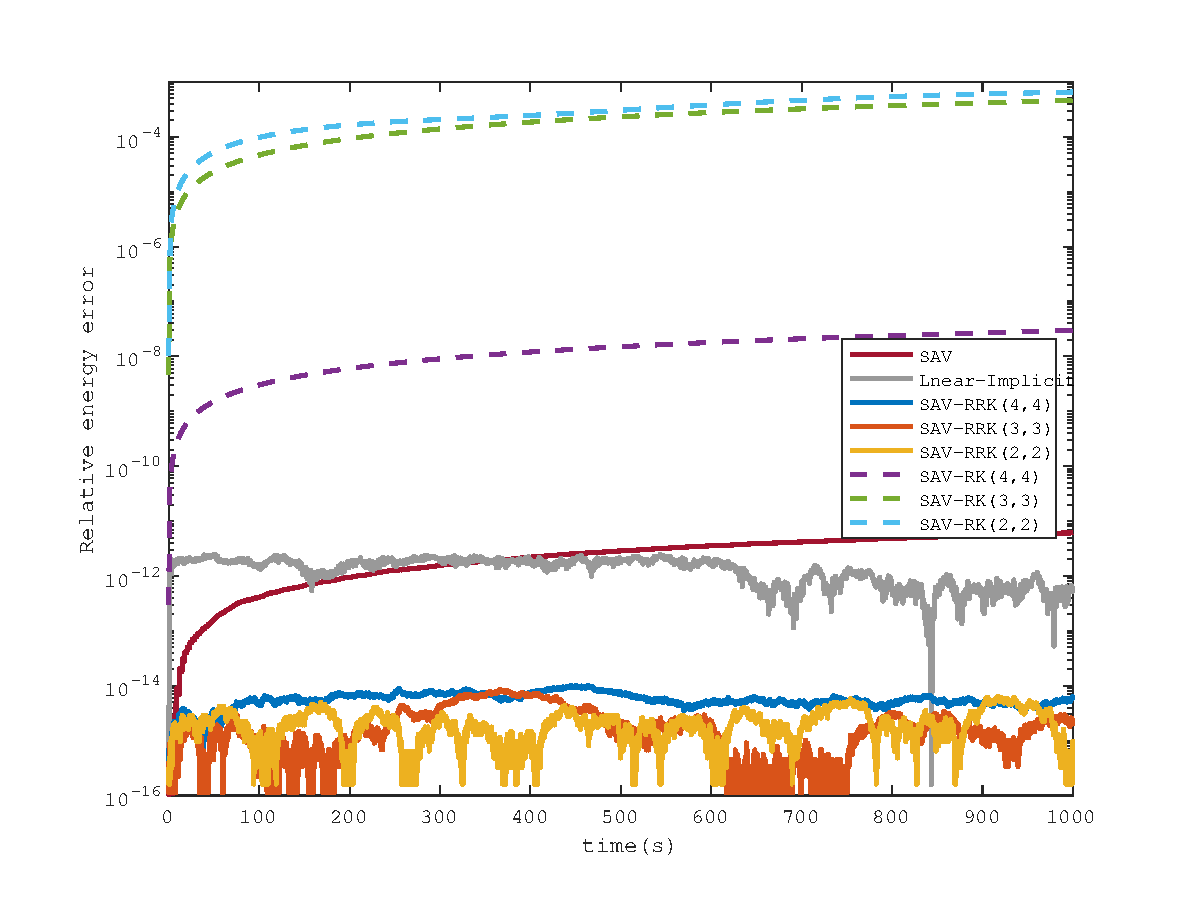
\includegraphics[width=0.5\textwidth]{./figures/exp1_energy6.eps}
		%\centerline{($a$) Temporal accuracy with $N=128.$}
		}\caption{当 $N=32$,$\tau=0.01$ 时,例 \ref{exp_SAVRRK:1} 中不同的 $\alpha$ 对应的相对能量误差.}
		\label{fig_SAVRRK:4-1}
		\end{center}
		\end{figure}
\end{frame}

\begin{frame}%\frametitle{数值算例}
	\begin{figure}[H]
		\begin{center}
		\subfigure[$\alpha=1.9$]{ \centering
		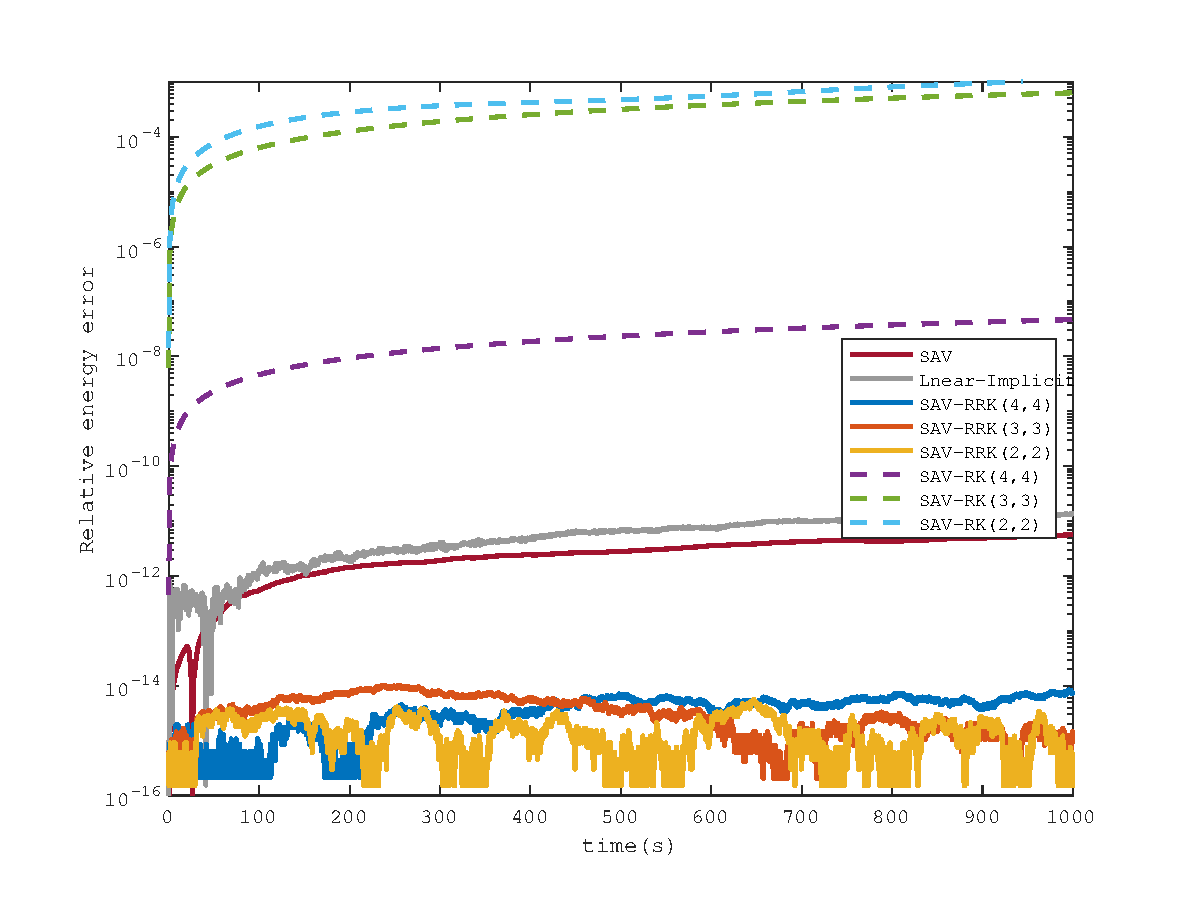
\includegraphics[width=0.5\textwidth]{./figures/exp1_energy9.eps}
		%\centerline{($b$) Spatial accuracy with $\tau = 10^{-3}.$}
		}\subfigure[$\alpha=2$]{ \centering
		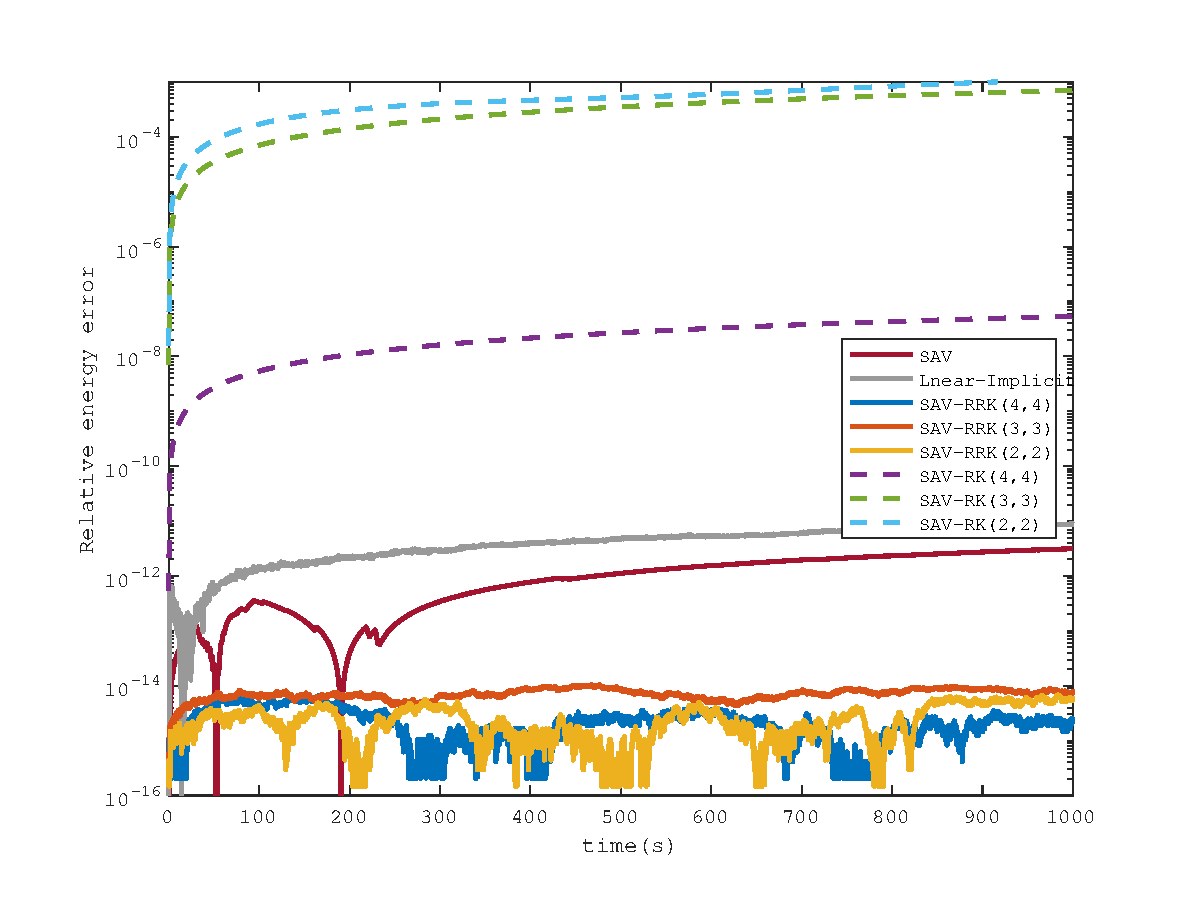
\includegraphics[width=0.5\textwidth]{./figures/exp1_energy2.eps}
		%\centerline{($a$) Temporal accuracy with $N=128.$}
		}
		% \caption{ Relative errors of energy with $N=32, \tau=0.01$ for different $\alpha$ in Example \ref{exp_SAVRRK:1}.}
		\caption{当 $N=32$,$\tau=0.01$ 时,例 \ref{exp_SAVRRK:1} 中不同的 $\alpha$ 对应的相对能量误差.}
		\label{fig_SAVRRK:4-2}
		\end{center}
		\end{figure}
\end{frame}
\begin{frame}\frametitle{数值算例}
	\begin{example}\label{exp_SAVRRK:2}
		考虑具有以下初值的 2维 NFSWEs:
		\begin{equation*}
		u(x, y, 0)=\operatorname{sech}\left(x^2+y^2\right), u_t(x, y, 0)=\sin (x+y) \operatorname{sech}\left(-2\left(x^2+y^2\right)\right),(x, y, t) \in \Omega \times[0, T],
		\end{equation*}
		其中 $\Omega=[-5,5] \times[-5,5]$.
		\end{example}
\end{frame}

\begin{frame}%\frametitle{数值算例}
	\begin{table}[H]\scriptsize
		\centering
		\caption{当 $N=4, T = 1$ 时,例 \ref{exp_SAVRRK:2} 在时间方向的误差和收敛阶}
		% \caption{Numerical errors and convergence order in time for Example \ref{exp_SAVRRK:2} when $N=4, T = 1$.}
		\begin{tabular}{lllllrlrlrlrlrl}
		\toprule
		\multicolumn{2}{l}{\multirow{2}[3]{*}{\textbf{RK(级,阶)}}} & \multicolumn{2}{l}{\multirow{2}[3]{*}{$\bm{\tau}$}} & \multicolumn{3}{c}{\textbf{SAV-RK}} &       & \multicolumn{3}{c}{\textbf{SAV-RRK}} &       & \multicolumn{3}{c}{\textbf{SAV-RRK(IDT)}} \\
		\cmidrule{5-7}\cmidrule{9-11}\cmidrule{13-15}    \multicolumn{2}{l}{} & \multicolumn{2}{l}{} & \textbf{Error($\tau$)} &       & \textbf{order} &       & \textbf{Error($\tau$)} &       & \textbf{order} &       & \textbf{Error($\tau$)} &       & \textbf{order} \\
		\hline
		\multicolumn{2}{l}{\multirow{5}[0]{*}{\textbf{RK(2,2)}}} & \multicolumn{2}{l}{0.1} & 3.0217E-03 &       & -     &       & 3.0102E-03 &       & -     &       & 1.5692E-02 &       & - \\
		\multicolumn{2}{l}{} & \multicolumn{2}{l}{0.05} & 7.4615E-04 &       & 2.0178  &       & 7.4702E-04 &       & 2.0106  &       & 9.6213E-03 &       & 0.7057  \\
		\multicolumn{2}{l}{} & \multicolumn{2}{l}{0.025} & 1.8513E-04 &       & 2.0109  &       & 1.8587E-04 &       & 2.0069  &       & 5.2472E-03 &       & 0.8747  \\
		\multicolumn{2}{l}{} & \multicolumn{2}{l}{0.0125} & 4.6090E-05 &       & 2.0060  &       & 4.6341E-05 &       & 2.0039  &       & 2.7312E-03 &       & 0.9420  \\
		\multicolumn{2}{l}{} & \multicolumn{2}{l}{0.00625} & 1.1497E-05 &       & 2.0032  &       & 1.1569E-05 &       & 2.0021  &       & 1.3923E-03 &       & 0.9721  \\
		\multicolumn{2}{l}{\multirow{5}[0]{*}{\textbf{RK(3,3)}}} & \multicolumn{2}{l}{0.1} & 1.2581E-04 &       & -     &       & 3.9379E-05 &       & -     &       & 3.2535E-03 &       & - \\
		\multicolumn{2}{l}{} & \multicolumn{2}{l}{0.05} & 1.6180E-05 &       & 2.9589  &       & 5.5726E-06 &       & 2.8210  &       & 7.9304E-04 &       & 2.0365  \\
		\multicolumn{2}{l}{} & \multicolumn{2}{l}{0.025} & 2.0532E-06 &       & 2.9783  &       & 7.4443E-07 &       & 2.9041  &       & 1.9546E-04 &       & 2.0205  \\
		\multicolumn{2}{l}{} & \multicolumn{2}{l}{0.0125} & 2.5863E-07 &       & 2.9889  &       & 9.6210E-08 &       & 2.9519  &       & 4.8500E-05 &       & 2.0108  \\
		\multicolumn{2}{l}{} & \multicolumn{2}{l}{0.00625} & 3.2454E-08 &       & 2.9944  &       & 1.2228E-08 &       & 2.9760  &       & 1.2078E-05 &       & 2.0056  \\
		\multicolumn{2}{l}{\multirow{5}[1]{*}{\textbf{RK(4,4)}}} & \multicolumn{2}{l}{0.1} & 7.9185E-06 &       & -     &       & 8.0508E-06 &       & -     &       & 3.4013E-05 &       & - \\
		\multicolumn{2}{l}{} & \multicolumn{2}{l}{0.05} & 4.9103E-07 &       & 4.0113  &       & 4.9644E-07 &       & 4.0194  &       & 3.3898E-06 &       & 3.3268  \\
		\multicolumn{2}{l}{} & \multicolumn{2}{l}{0.025} & 3.0531E-08 &       & 4.0075  &       & 3.0805E-08 &       & 4.0104  &       & 3.6901E-07 &       & 3.1995  \\
		\multicolumn{2}{l}{} & \multicolumn{2}{l}{0.0125} & 1.9026E-09 &       & 4.0042  &       & 1.9182E-09 &       & 4.0054  &       & 4.2681E-08 &       & 3.1120  \\
		\multicolumn{2}{l}{} & \multicolumn{2}{l}{0.00625} & 1.1873E-10 &       & 4.0022  &       & 1.1966E-10 &       & 4.0027  &       & 5.1191E-09 &       & 3.0596  \\
		\bottomrule
		\end{tabular}%
		\label{tab_SAVRRK:6-2}%
		\end{table}%
\end{frame}

\begin{frame}%\frametitle{数值算例}
	\begin{figure}[H]
		\begin{center}
		\subfigure[$\max_m\left|\gamma_m-1\right|$]{ \centering
		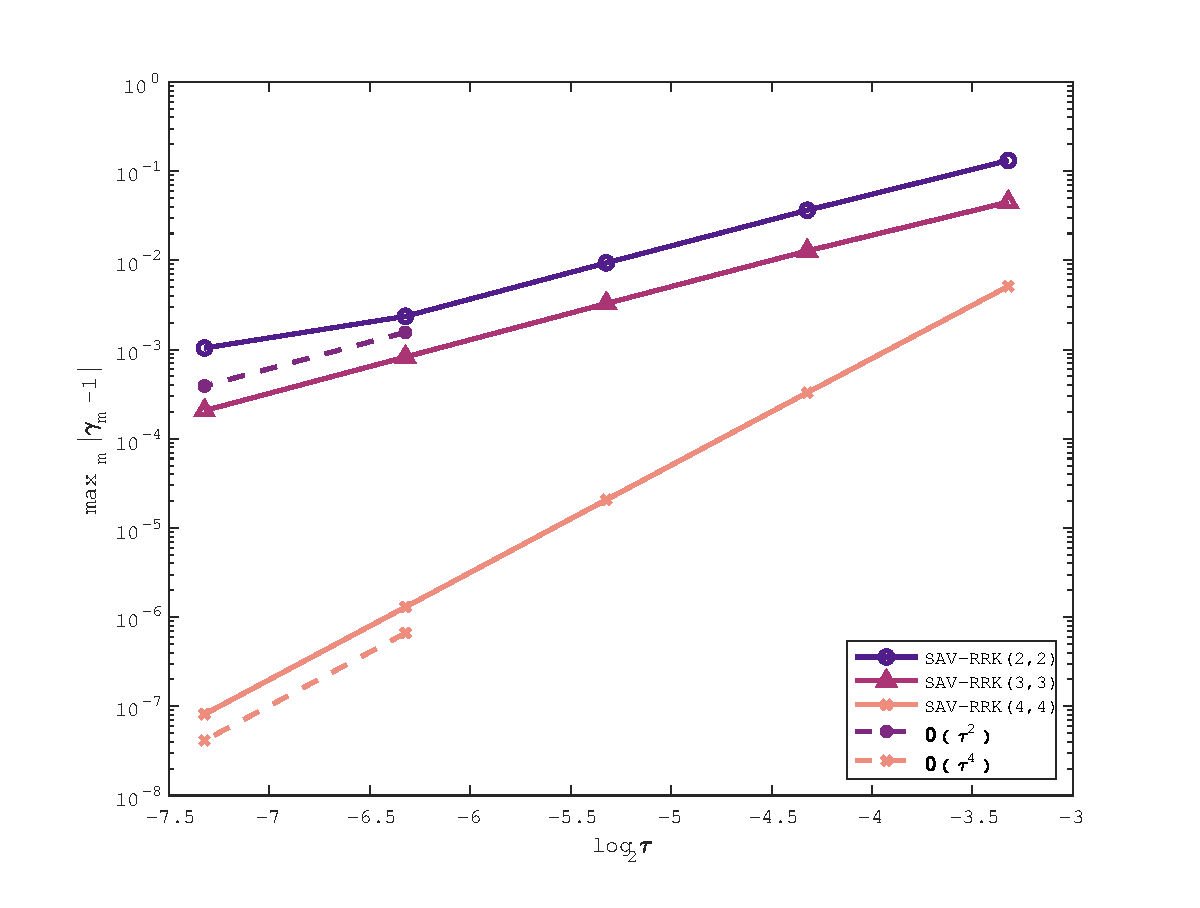
\includegraphics[width=0.5\textwidth]{./figures/exp2_r.eps}
		%\centerline{($b$) Spatial accuracy with $\tau = 10^{-3}.$}
		}\subfigure[$\max_m\left|S_m(1)\right|$]{ \centering
		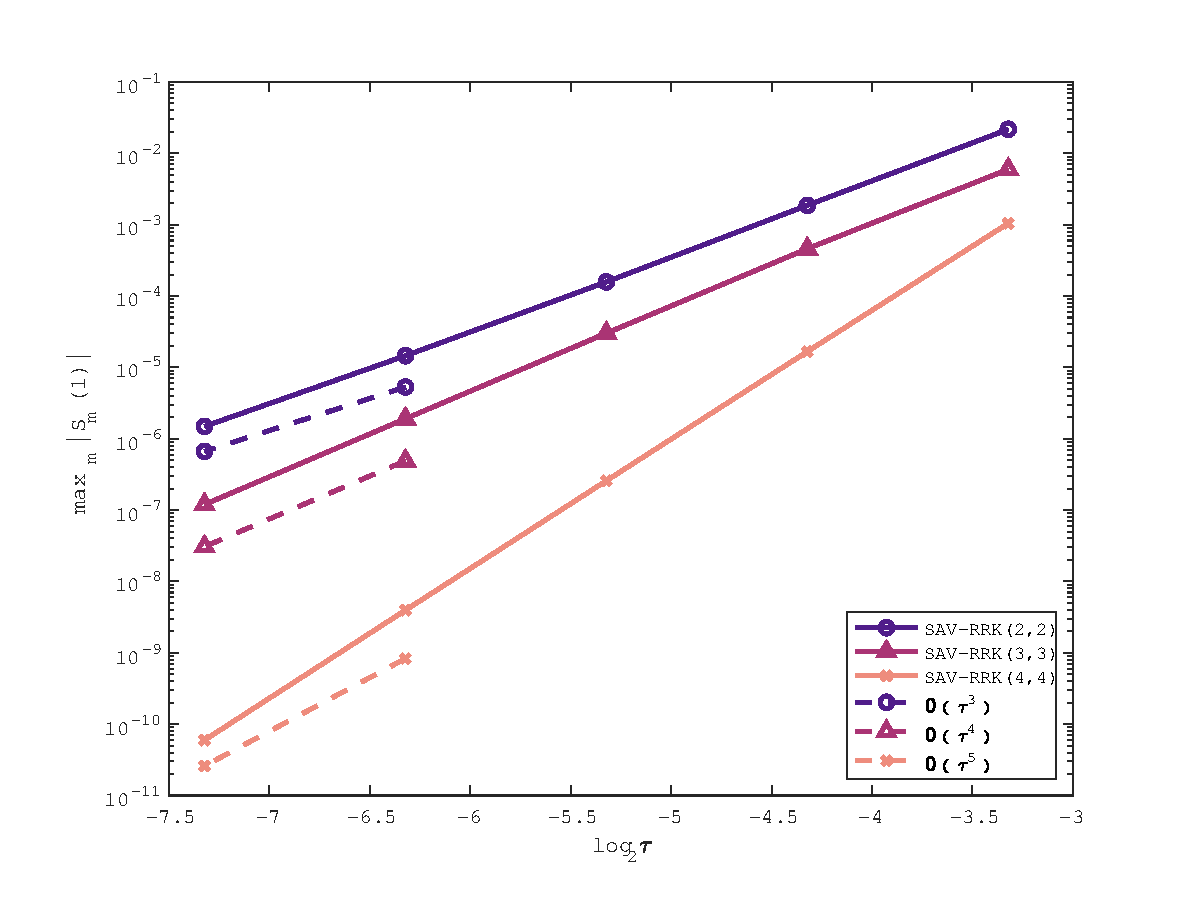
\includegraphics[width=0.5\textwidth]{./figures/exp2_s.eps}
		%\centerline{($a$) Temporal accuracy with $N=128.$}
		}
		% \caption{$\max _m\left|\gamma_m-1\right|$ and $\max_m\left|S_m(1)\right|$ for some relaxation (RT) methods in Example \ref{exp_SAVRRK:2}.}
		\caption{例 \ref{exp_SAVRRK:2}中一些松弛格式(RT)所对应的$\max_m\left|\gamma_m-1\right|$ 和 $\max_m\left|S_m(1)\right|$.}
		\label{fig_SAVRRK:2-1}
		\end{center}
		\end{figure}
\end{frame}

\begin{frame}%\frametitle{数值算例}
	\begin{figure}[H]
		\begin{center}
		\subfigure[$\alpha=1.3$]{ \centering
		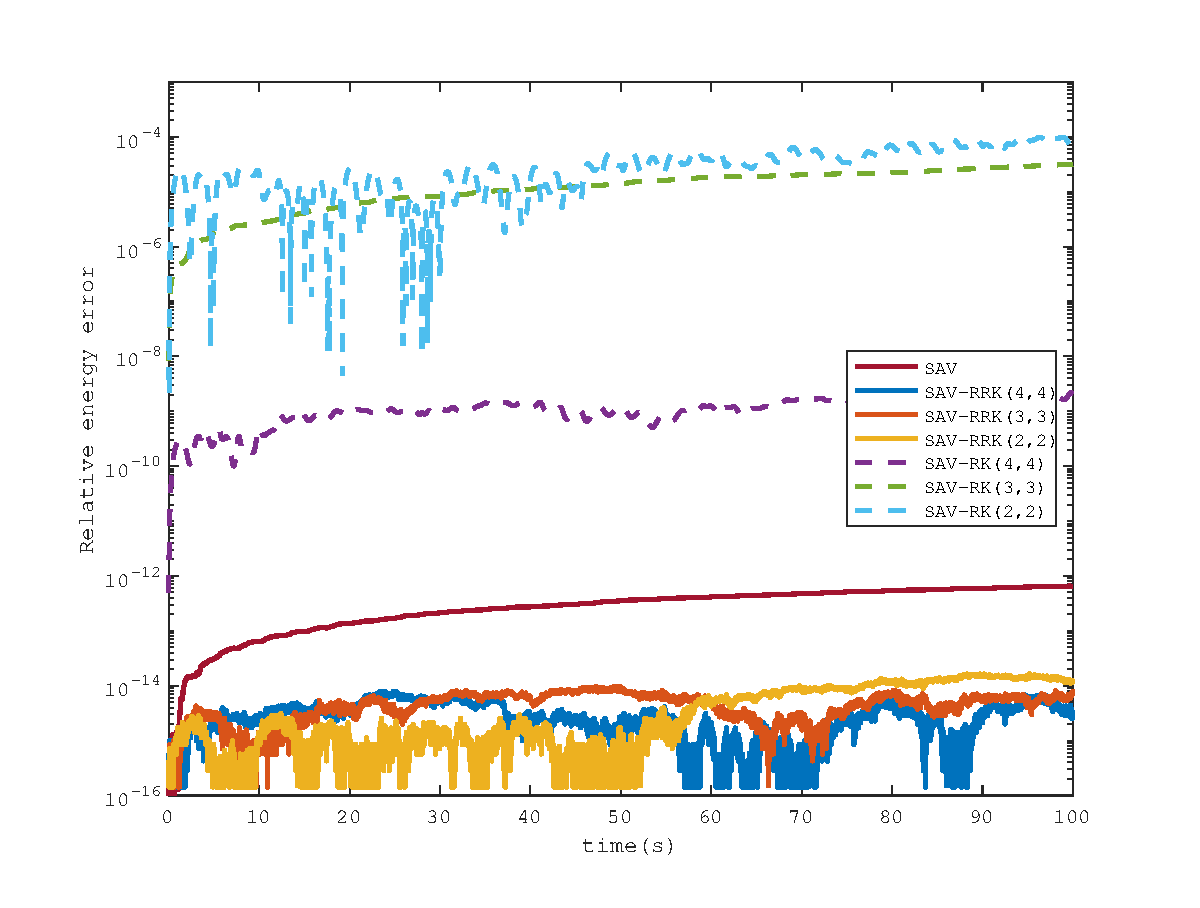
\includegraphics[width=0.5\textwidth]{./figures/exp2_energy3.eps}
		%\centerline{($b$) Spatial accuracy with $\tau = 10^{-3}.$}
		}\subfigure[$\alpha=1.6$]{ \centering
		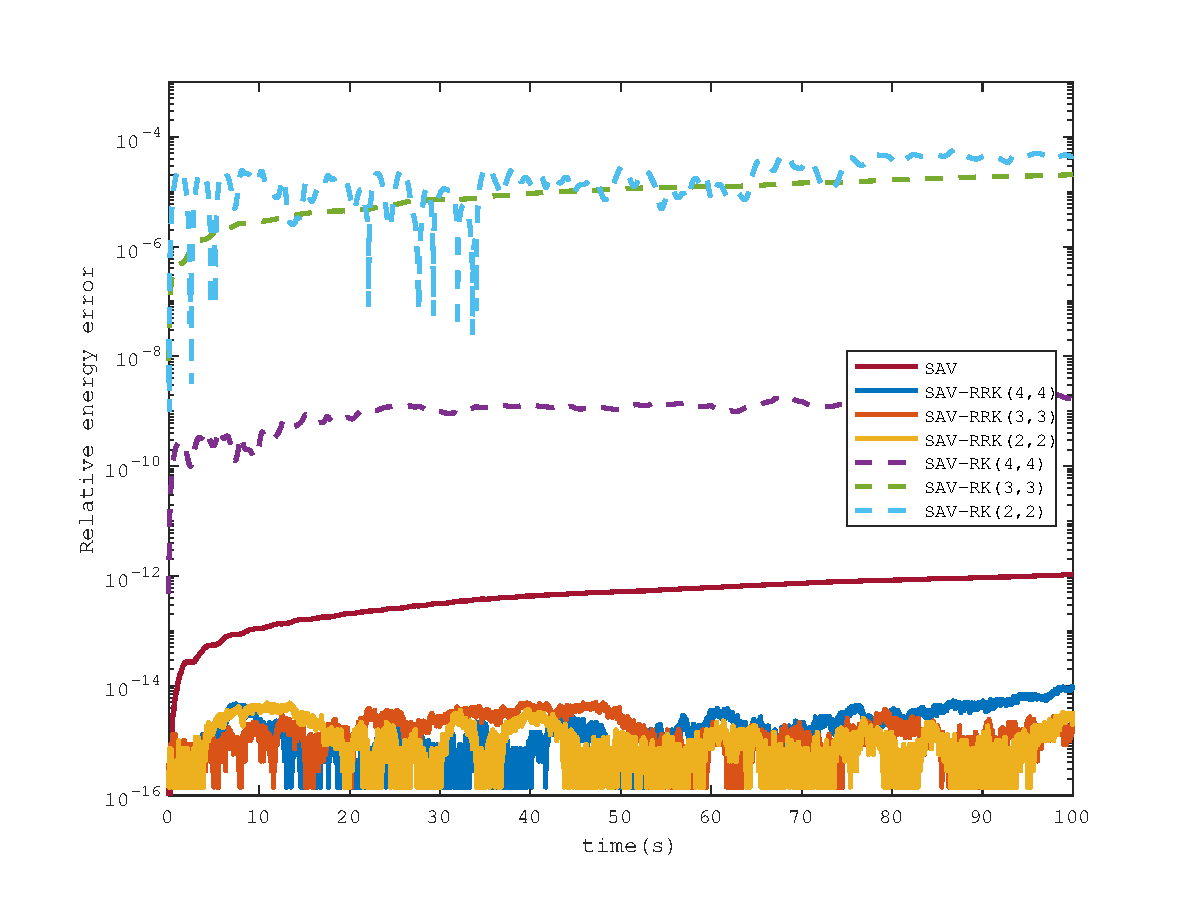
\includegraphics[width=0.5\textwidth]{./figures/exp2_energy6.eps}
		%\centerline{($a$) Temporal accuracy with $N=128.$}
		}\caption{当 $N=4, \tau=0.01$ 时,例 \ref{exp_SAVRRK:2} 中不同的 $\alpha$ 对应的相对能量误差.}
		\label{fig_SAVRRK:2-4}
		\end{center}
		\end{figure}
\end{frame}

\begin{frame}%\frametitle{数值算例}
	\begin{figure}[H]
		\begin{center}
		\subfigure[$\alpha=1.9$]{ \centering
		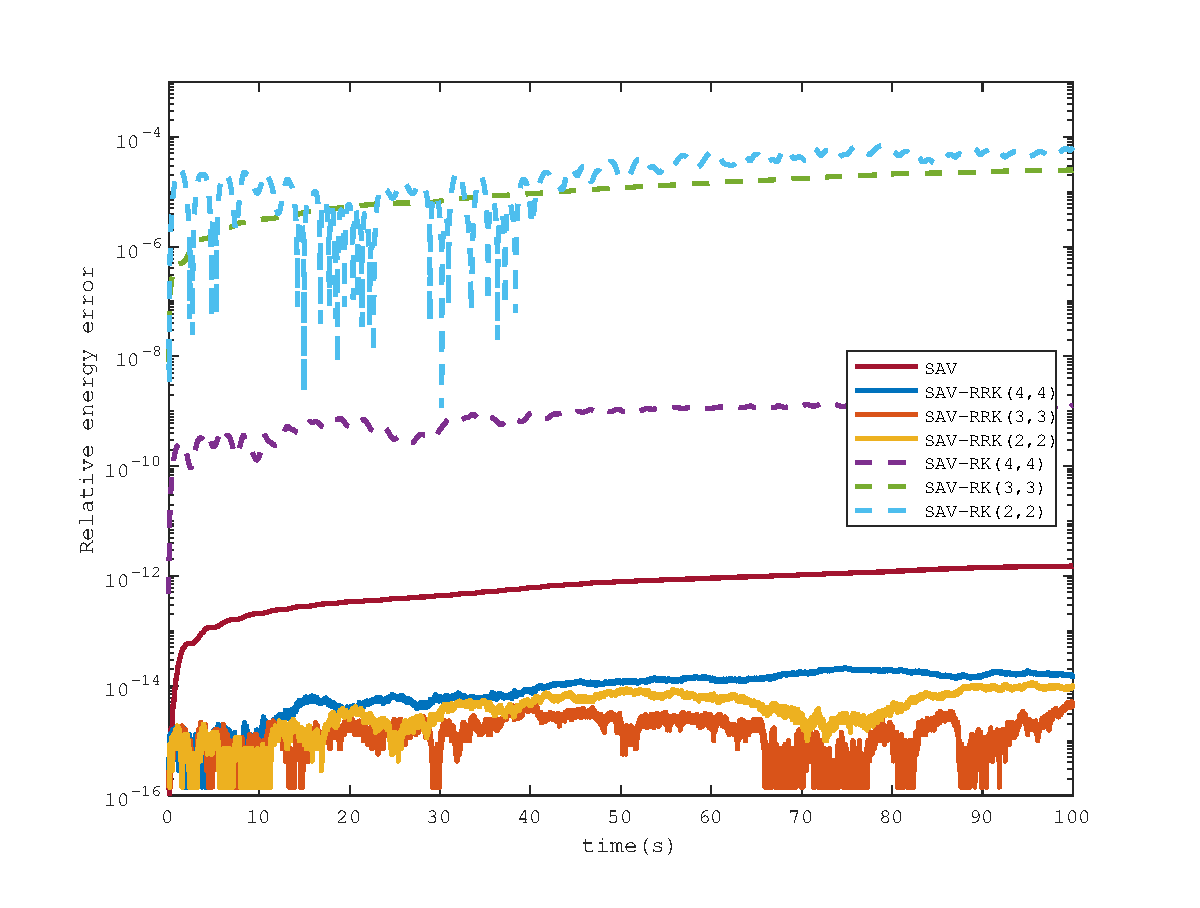
\includegraphics[width=0.5\textwidth]{./figures/exp2_energy9.eps}
		%\centerline{($b$) Spatial accuracy with $\tau = 10^{-3}.$}
		}\subfigure[$\alpha=2$]{ \centering
		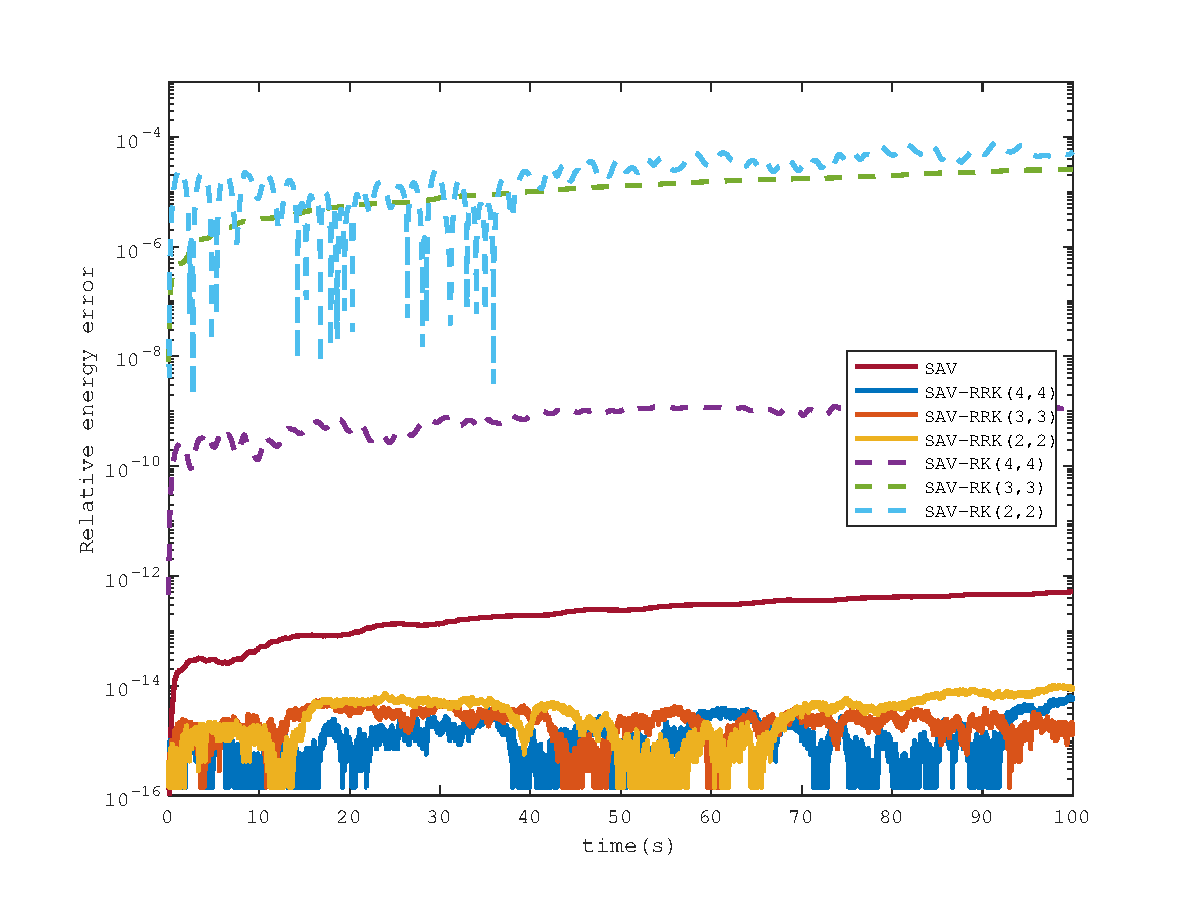
\includegraphics[width=0.5\textwidth]{./figures/exp2_energy2.eps}
		%\centerline{($a$) Temporal accuracy with $N=128.$}
		}
		% \caption{ Relative errors of energy with $N=4, \tau=0.01$ for different $\alpha$ in Example \ref{exp_SAVRRK:2}.}
		\caption{当 $N=4, \tau=0.01$ 时,例 \ref{exp_SAVRRK:2} 中不同的 $\alpha$ 对应的相对能量误差.}
		\label{fig_SAVRRK:2-4}
		\end{center}
		\end{figure}
\end{frame}
\begin{frame}\frametitle{数值算例}
	\begin{example}\label{exp_SAVRRK:3}
		考虑二维非线性分数阶波动方程\cite{wangUnconditionalEnergyDissipation2021} 
		\begin{equation}
		\begin{cases}
		& u_{t t}+(-\Delta)^{\frac{\alpha}{2}} u+F^{\prime}(u)=0,(x, y, t) \in \Omega \times(0, T],\\
		& u(x, y, 0)=\frac{1}{2} \arctan \left(\exp \left(-\sqrt{x^2+y^2}\right)\right), u_t(x, y, 0)=0,
		\end{cases}
		\end{equation}
		其中 $\Omega=(-10,10) \times(-10,10)$.
		\end{example}
		
		取势能 $F(u)=u^2\left(\frac{1}{4} u^2-\frac{1}{2}\right)$.
\end{frame}

\begin{frame}%\frametitle{数值算例}
	\begin{table}[H]\scriptsize
		\centering
		% \caption{Numerical errors and convergence order in time for Example \ref{exp_SAVRRK:3} when $N=4, T = 1$.}
		\caption{当 $N=4, T = 1$ 时,例 \ref{exp_SAVRRK:3} 在时间方向的误差和收敛阶}
		\begin{tabular}{lllllrlrlrlrlrl}
		\toprule
		\multicolumn{2}{l}{\multirow{2}[3]{*}{\textbf{RK(级,阶)}}} & \multicolumn{2}{l}{\multirow{2}[3]{*}{$\bm{\tau}$}} & \multicolumn{3}{c}{\textbf{SAV-RK}} &       & \multicolumn{3}{c}{\textbf{SAV-RRK(RT)}} &       & \multicolumn{3}{c}{\textbf{SAV-RRK(IDT)}} \\
		\cmidrule{5-7}\cmidrule{9-11}\cmidrule{13-15}    \multicolumn{2}{l}{} & \multicolumn{2}{l}{} & \textbf{Error($\tau$)} &       & \textbf{order} &       & \textbf{Error($\tau$)} &       & \textbf{order} &       & \textbf{Error($\tau$)} &       & \textbf{order} \\
		\hline
		\multicolumn{2}{l}{\multirow{5}[0]{*}{\textbf{RK(2,2)}}} & \multicolumn{2}{l}{0.1} & 1.3395E-03 &       & -     &       & 3.3870E-03 &       & -     &       & 2.1470E-02 &       & - \\
		\multicolumn{2}{l}{} & \multicolumn{2}{l}{0.05} & 3.4360E-04 &       & 1.9628  &       & 8.1480E-04 &       & 2.0555  &       & 1.0960E-02 &       & 0.9701  \\
		\multicolumn{2}{l}{} & \multicolumn{2}{l}{0.025} & 8.6945E-05 &       & 1.9826  &       & 1.9951E-04 &       & 2.0300  &       & 5.5113E-03 &       & 0.9918  \\
		\multicolumn{2}{l}{} & \multicolumn{2}{l}{0.0125} & 2.1865E-05 &       & 1.9915  &       & 4.9347E-05 &       & 2.0154  &       & 2.7600E-03 &       & 0.9977  \\
		\multicolumn{2}{l}{} & \multicolumn{2}{l}{0.00625} & 5.4823E-06 &       & 1.9958  &       & 1.2270E-05 &       & 2.0078  &       & 1.3807E-03 &       & 0.9993  \\
		\multicolumn{2}{l}{\multirow{5}[0]{*}{\textbf{RK(3,3)}}} & \multicolumn{2}{l}{0.1} & 3.5168E-05 &       & -     &       & 4.3927E-05 &       & -     &       & 3.8213E-04 &       & - \\
		\multicolumn{2}{l}{} & \multicolumn{2}{l}{0.05} & 4.3533E-06 &       & 3.0141  &       & 5.4825E-06 &       & 3.0022  &       & 8.0473E-05 &       & 2.2475  \\
		\multicolumn{2}{l}{} & \multicolumn{2}{l}{0.025} & 5.3902E-07 &       & 3.0137  &       & 6.8378E-07 &       & 3.0032  &       & 1.8560E-05 &       & 2.1163  \\
		\multicolumn{2}{l}{} & \multicolumn{2}{l}{0.0125} & 6.7058E-08 &       & 3.0068  &       & 8.5344E-08 &       & 3.0022  &       & 4.4475E-06 &       & 2.0611  \\
		\multicolumn{2}{l}{} & \multicolumn{2}{l}{0.00625} & 8.3615E-09 &       & 3.0036  &       & 1.0659E-08 &       & 3.0012  &       & 1.0883E-06 &       & 2.0309  \\
		\multicolumn{2}{l}{\multirow{5}[1]{*}{\textbf{RK(4,4)}}} & \multicolumn{2}{l}{0.1} & 5.3561E-07 &       & -     &       & 3.2716E-06 &       & -     &       & 3.7745E-05 &       & - \\
		\multicolumn{2}{l}{} & \multicolumn{2}{l}{0.05} & 3.6438E-08 &       & 3.8777  &       & 2.0654E-07 &       & 3.9855  &       & 4.8050E-06 &       & 2.9737  \\
		\multicolumn{2}{l}{} & \multicolumn{2}{l}{0.025} & 2.3735E-09 &       & 3.9403  &       & 1.2898E-08 &       & 4.0012  &       & 6.0237E-07 &       & 2.9958  \\
		\multicolumn{2}{l}{} & \multicolumn{2}{l}{0.0125} & 1.5146E-10 &       & 3.9700  &       & 8.0476E-10 &       & 4.0024  &       & 7.5303E-08 &       & 2.9999  \\
		\multicolumn{2}{l}{} & \multicolumn{2}{l}{0.00625} & 9.5636E-12 &       & 3.9853  &       & 5.0241E-11 &       & 4.0016  &       & 9.4105E-09 &       & 3.0004  \\
		\bottomrule
		\end{tabular}%
		\label{tab_SAVRRK:6-3}%
		\end{table}%
\end{frame}

\begin{frame}%\frametitle{数值算例}
	\begin{figure}[H]
		\begin{center}
		\subfigure[$\alpha=1.3$]{ \centering
		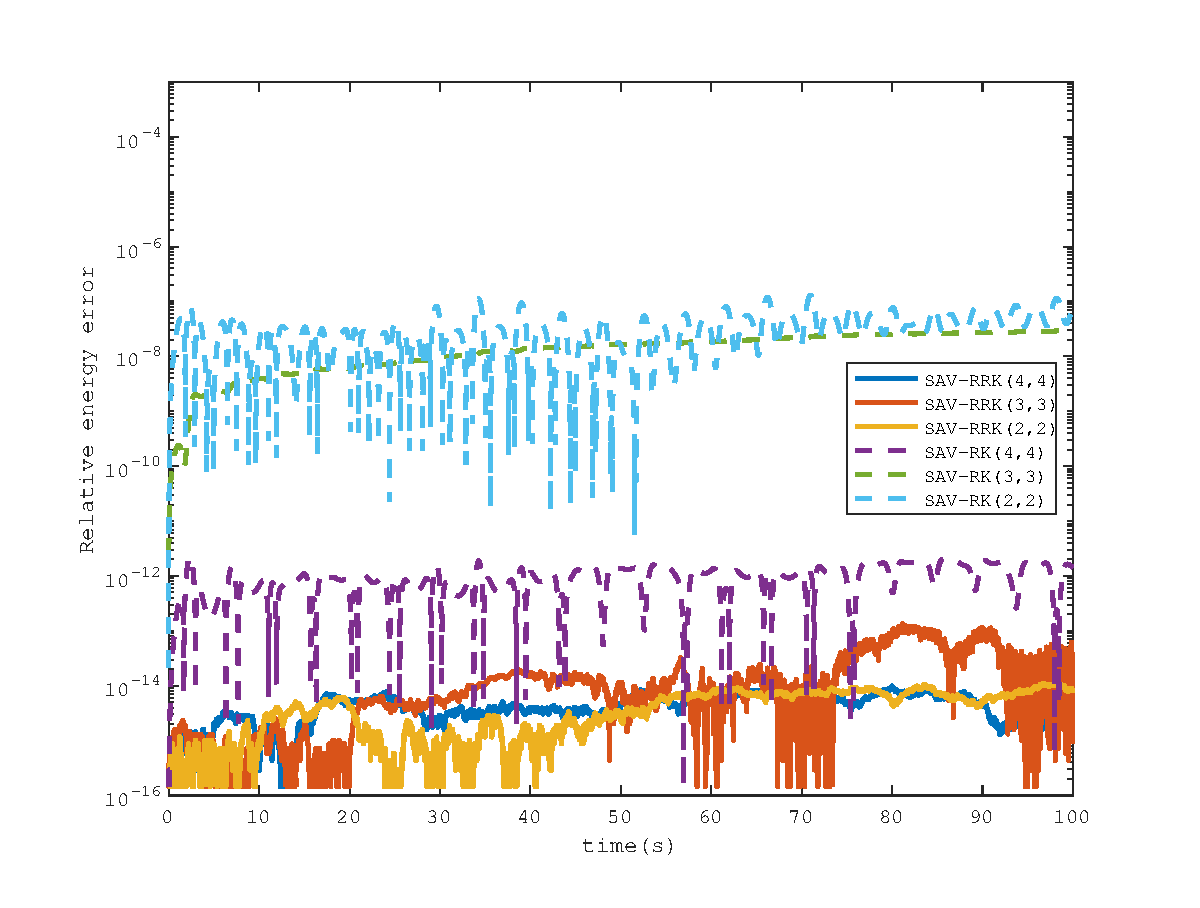
\includegraphics[width=0.5\textwidth]{./figures/exp3_energy3.eps}
		%\centerline{($b$) Spatial accuracy with $\tau = 10^{-3}.$}
		}\subfigure[$\alpha=1.6$]{ \centering
		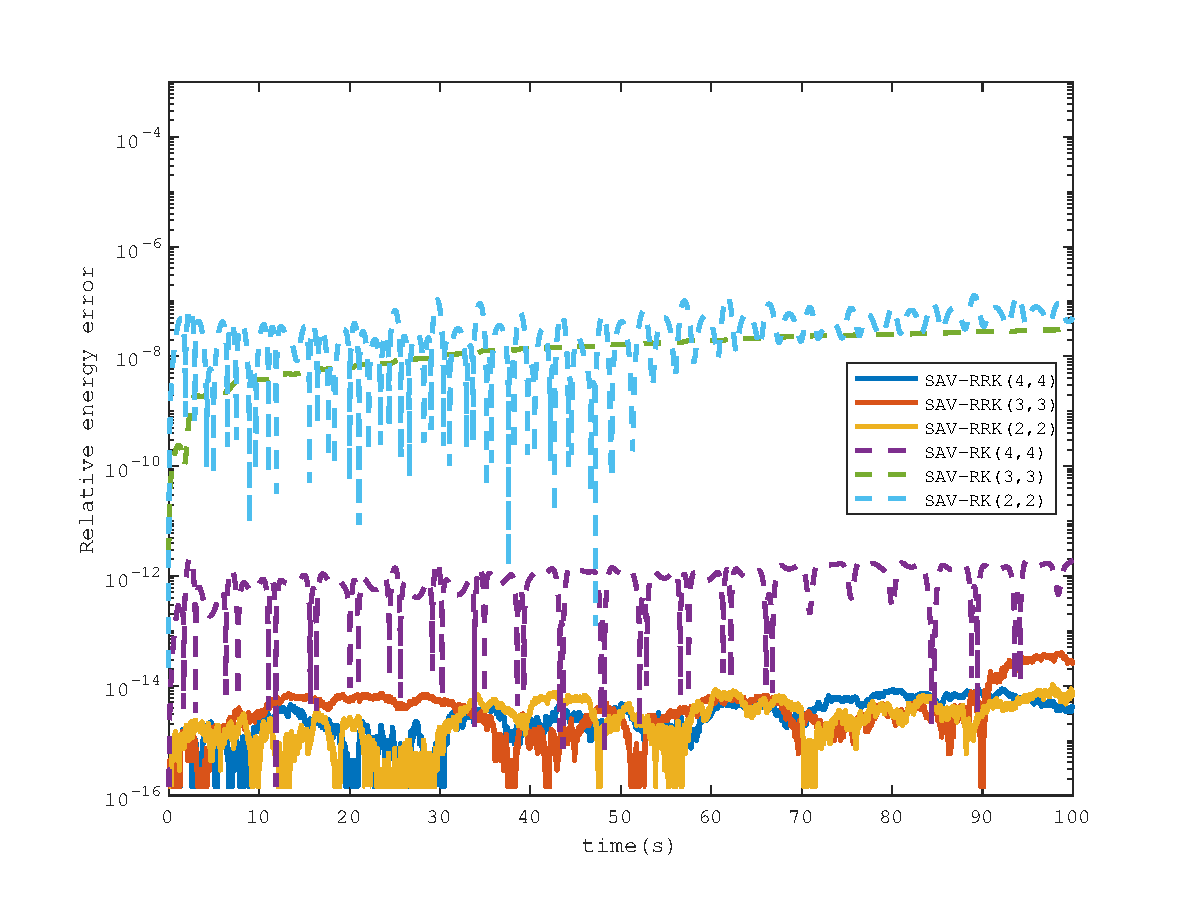
\includegraphics[width=0.5\textwidth]{./figures/exp3_energy6.eps}
		%\centerline{($a$) Temporal accuracy with $N=128.$}
		}\caption{当 $N=4, \tau=0.01$ 时,例 \ref{exp_SAVRRK:3} 中不同的 $\alpha$ 对应的相对能量误差.}
		\label{fig_SAVRRK:3-4}
		\end{center}
		\end{figure}
\end{frame}

\begin{frame}%\frametitle{数值算例}
	\begin{figure}[H]
		\begin{center}
		\subfigure[$\alpha=1.9$]{ \centering
		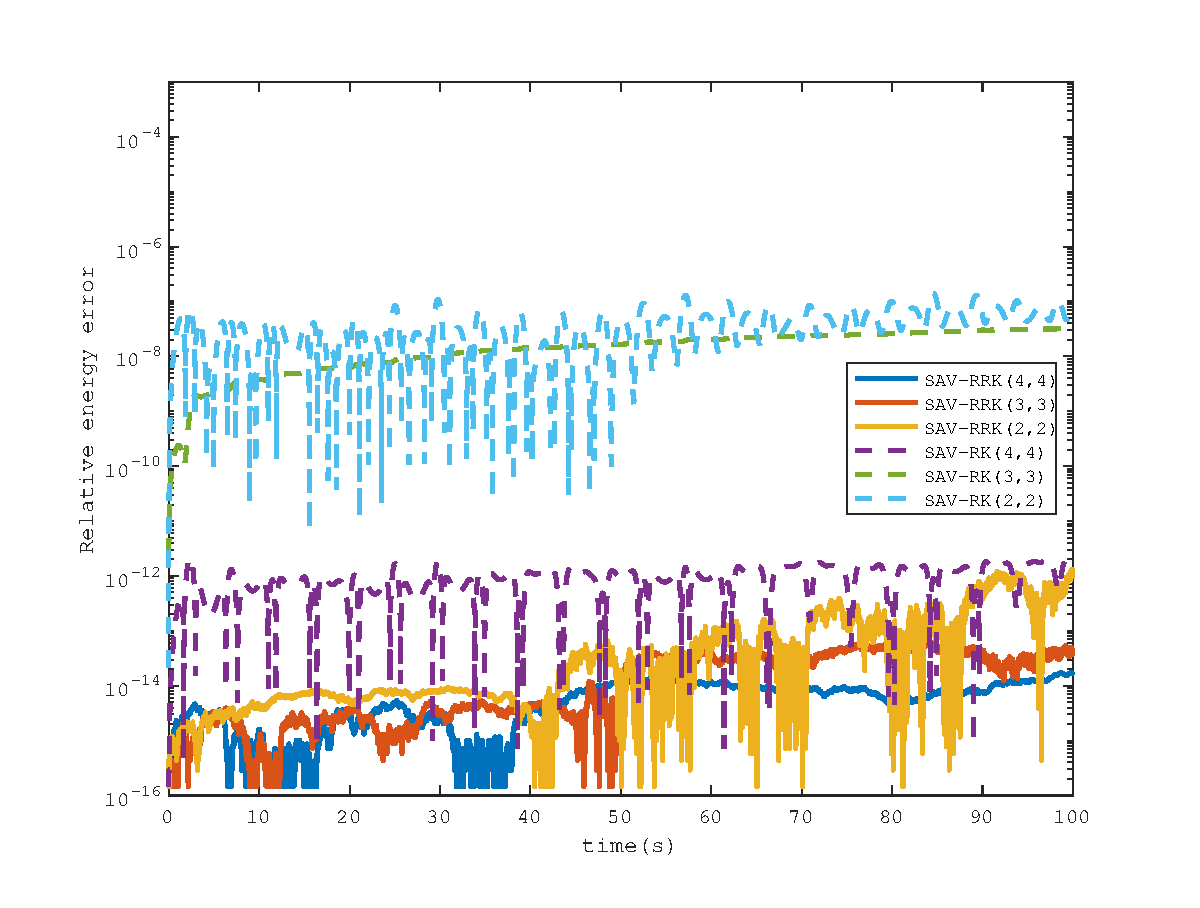
\includegraphics[width=0.5\textwidth]{./figures/exp3_energy9.eps}
		%\centerline{($b$) Spatial accuracy with $\tau = 10^{-3}.$}
		}\subfigure[$\alpha=2$]{ \centering
		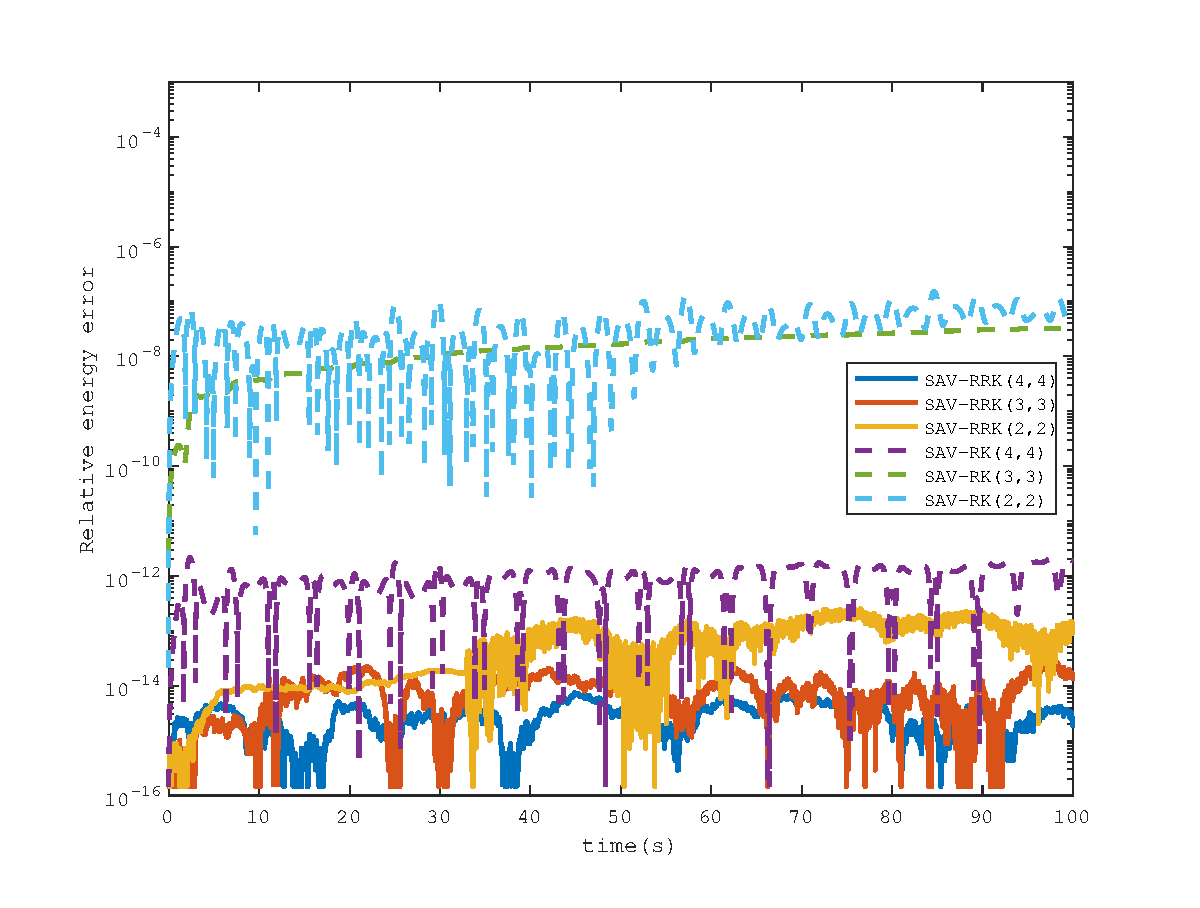
\includegraphics[width=0.5\textwidth]{./figures/exp3_energy2.eps}
		%\centerline{($a$) Temporal accuracy with $N=128.$}
		}
		% \caption{ Relative errors of energy with $N=4, \tau=0.01$ for different $\alpha$ in Example \ref{exp_SAVRRK:3}.}
		\caption{当 $N=4, \tau=0.01$ 时,例 \ref{exp_SAVRRK:3} 中不同的 $\alpha$ 对应的相对能量误差.}
		\label{fig_SAVRRK:3-4}
		\end{center}
		\end{figure}
\end{frame}

\begin{frame}\frametitle{数值算例}
	\begin{example}\label{exp_SAVRRK:4}
		考虑二维分数阶Klein-Gordon-Schr{\"o}dinger方程\cite{fuStructurepreservingAlgorithmsTwodimensional2020} 
		\begin{equation}
		\begin{cases}
		\mathrm{i} \partial_t u-\frac{1}{2}(-\Delta)^{\frac{\alpha}{2}} u+u \phi=0,(x, y, t) \in \Omega \times(0, T],\\
		\partial_{t t} \phi+(-\Delta)^{\frac{\beta}{2}} \phi+\phi-|u|^2=0, (x, y, t) \in \Omega \times(0, T],
		\end{cases}
		\end{equation}
		初始条件为
		\begin{equation}
			\begin{aligned}
				u(x, y, 0)&=(1+\mathrm{i}) \exp \left(-|\boldsymbol{x}|^2\right),~~\phi(x, y, 0)=\operatorname{sech}\left(|\boldsymbol{x}|^2\right),\\
				\partial_t \phi(x, y, 0)&=\sin (x+y) \operatorname{sech}\left(-2|\boldsymbol{x}|^2\right),
			\end{aligned}
		\end{equation}
		其中 $\Omega=[-10,10] \times[-10,10]$.
		\end{example}
\end{frame}

\begin{frame}%\frametitle{数值算例}
	\begin{table}[H]\scriptsize
		\centering
		% \caption{Numerical errors and convergence order in time for Example \ref{exp_SAVRRK:4} when $N=4, T = 1$.}
		\caption{当 $N=4, T = 1$ 时,例 \ref{exp_SAVRRK:4} 在时间方向的误差和收敛阶}
		\begin{tabular}{lllllrlrlrlrlrl}
		\toprule
		\multicolumn{2}{l}{\multirow{2}[3]{*}{\textbf{RK(级,阶)}}} & \multicolumn{2}{l}{\multirow{2}[3]{*}{$\bm{\tau}$}} & \multicolumn{3}{c}{\textbf{SAV-RK}} &       & \multicolumn{3}{c}{\textbf{SAV-RRK(RT)}} &       & \multicolumn{3}{c}{\textbf{SAV-RRK(IDT)}} \\
		\cmidrule{5-7}\cmidrule{9-11}\cmidrule{13-15}    \multicolumn{2}{l}{} & \multicolumn{2}{l}{} & \textbf{Error($\tau$)} &       & \textbf{order} &       & \textbf{Error($\tau$)} &       & \textbf{order} &       & \textbf{Error($\tau$)} &       & \textbf{order} \\
		\hline
		\multicolumn{2}{l}{\multirow{5}[0]{*}{\textbf{RK(2,2)}}} & \multicolumn{2}{l}{0.1} & 1.1875E-03 &       & -     &       & 1.8837E-03 &       & -     &       & 9.5325E-03 &       & - \\
		\multicolumn{2}{l}{} & \multicolumn{2}{l}{0.05} & 2.7648E-04 &       & 2.1026  &       & 5.0394E-04 &       & 1.9023  &       & 6.7134E-03 &       & 0.5058  \\
		\multicolumn{2}{l}{} & \multicolumn{2}{l}{0.025} & 6.6514E-05 &       & 2.0555  &       & 1.3036E-04 &       & 1.9508  &       & 3.8805E-03 &       & 0.7908  \\
		\multicolumn{2}{l}{} & \multicolumn{2}{l}{0.0125} & 1.6300E-05 &       & 2.0288  &       & 3.3151E-05 &       & 1.9754  &       & 2.0757E-03 &       & 0.9026  \\
		\multicolumn{2}{l}{} & \multicolumn{2}{l}{0.00625} & 4.0339E-06 &       & 2.0146  &       & 8.3587E-06 &       & 1.9877  &       & 1.0723E-03 &       & 0.9529  \\
		\multicolumn{2}{l}{\multirow{5}[0]{*}{\textbf{RK(3,3)}}} & \multicolumn{2}{l}{0.1} & 8.7748E-05 &       & -     &       & 1.9567E-04 &       & -     &       & 3.1789E-03 &       & - \\
		\multicolumn{2}{l}{} & \multicolumn{2}{l}{0.05} & 1.1471E-05 &       & 2.9354  &       & 2.4630E-05 &       & 2.9900  &       & 8.2646E-04 &       & 1.9435  \\
		\multicolumn{2}{l}{} & \multicolumn{2}{l}{0.025} & 1.4684E-06 &       & 2.9657  &       & 3.0916E-06 &       & 2.9940  &       & 2.1079E-04 &       & 1.9712  \\
		\multicolumn{2}{l}{} & \multicolumn{2}{l}{0.0125} & 1.8580E-07 &       & 2.9824  &       & 3.8731E-07 &       & 2.9968  &       & 5.3231E-05 &       & 1.9854  \\
		\multicolumn{2}{l}{} & \multicolumn{2}{l}{0.00625} & 2.3370E-08 &       & 2.9911  &       & 4.8471E-08 &       & 2.9983  &       & 1.3375E-05 &       & 1.9927  \\
		\multicolumn{2}{l}{\multirow{5}[1]{*}{\textbf{RK(4,4)}}} & \multicolumn{2}{l}{0.1} & 3.0741E-06 &       & -     &       & 4.0627E-06 &       & -     &       & 1.0278E-04 &       & - \\
		\multicolumn{2}{l}{} & \multicolumn{2}{l}{0.05} & 1.9959E-07 &       & 3.9450  &       & 2.6020E-07 &       & 3.9647  &       & 1.3195E-05 &       & 2.9615  \\
		\multicolumn{2}{l}{} & \multicolumn{2}{l}{0.025} & 1.2698E-08 &       & 3.9744  &       & 1.6461E-08 &       & 3.9825  &       & 1.6711E-06 &       & 2.9811  \\
		\multicolumn{2}{l}{} & \multicolumn{2}{l}{0.0125} & 8.0044E-10 &       & 3.9876  &       & 1.0350E-09 &       & 3.9913  &       & 2.1024E-07 &       & 2.9906  \\
		\multicolumn{2}{l}{} & \multicolumn{2}{l}{0.00625} & 5.0238E-11 &       & 3.9939  &       & 6.4882E-11 &       & 3.9957  &       & 2.6365E-08 &       & 2.9953  \\
		\bottomrule
		\end{tabular}%
		\label{tab_SAVRRK:6-4}%
		\end{table}%
\end{frame}

\begin{frame}%\frametitle{数值算例}
	\begin{figure}[H]
		\begin{center}
		\subfigure[$\alpha,\beta=1.3$]{ \centering
		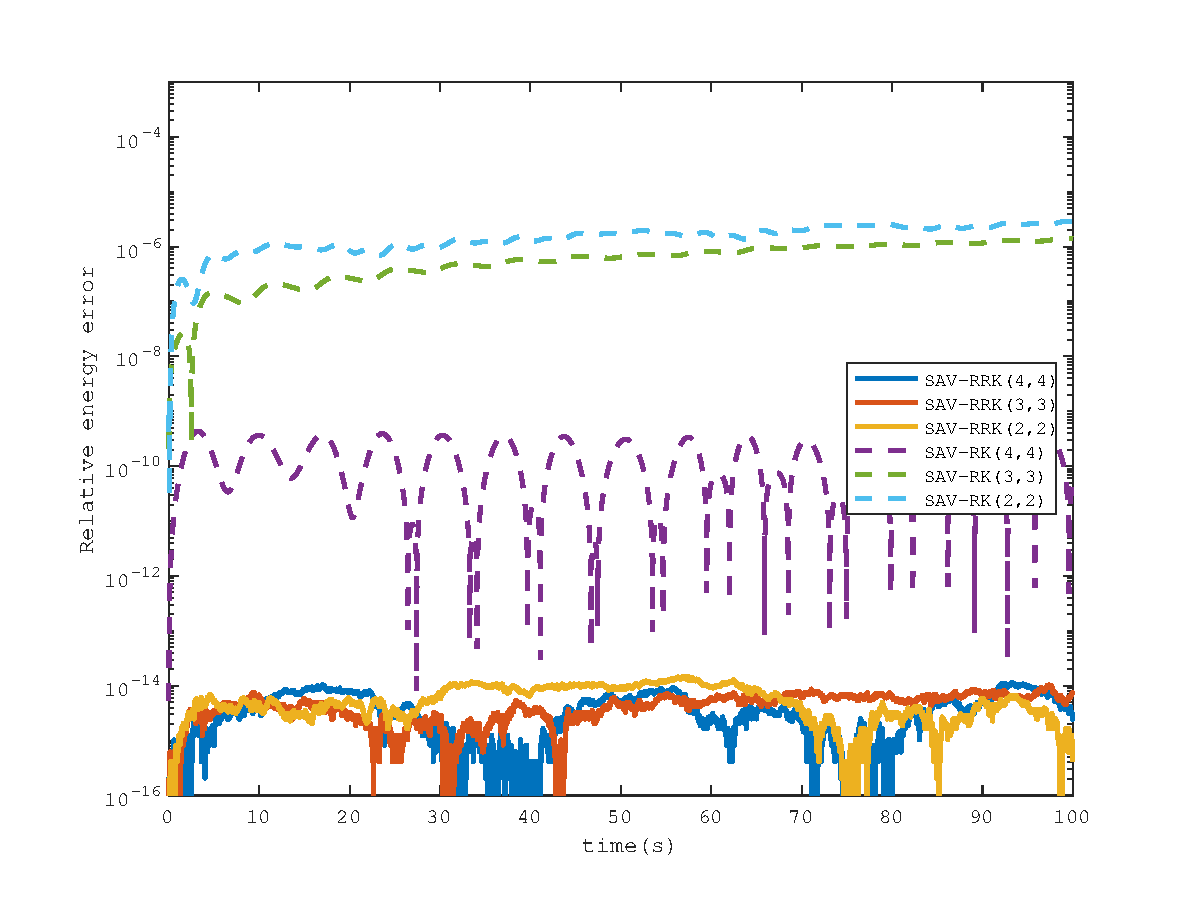
\includegraphics[width=0.5\textwidth]{./figures/exp4_energy3.eps}
		%\centerline{($b$) Spatial accuracy with $\tau = 10^{-3}.$}
		}\subfigure[$\alpha,\beta=1.6$]{ \centering
		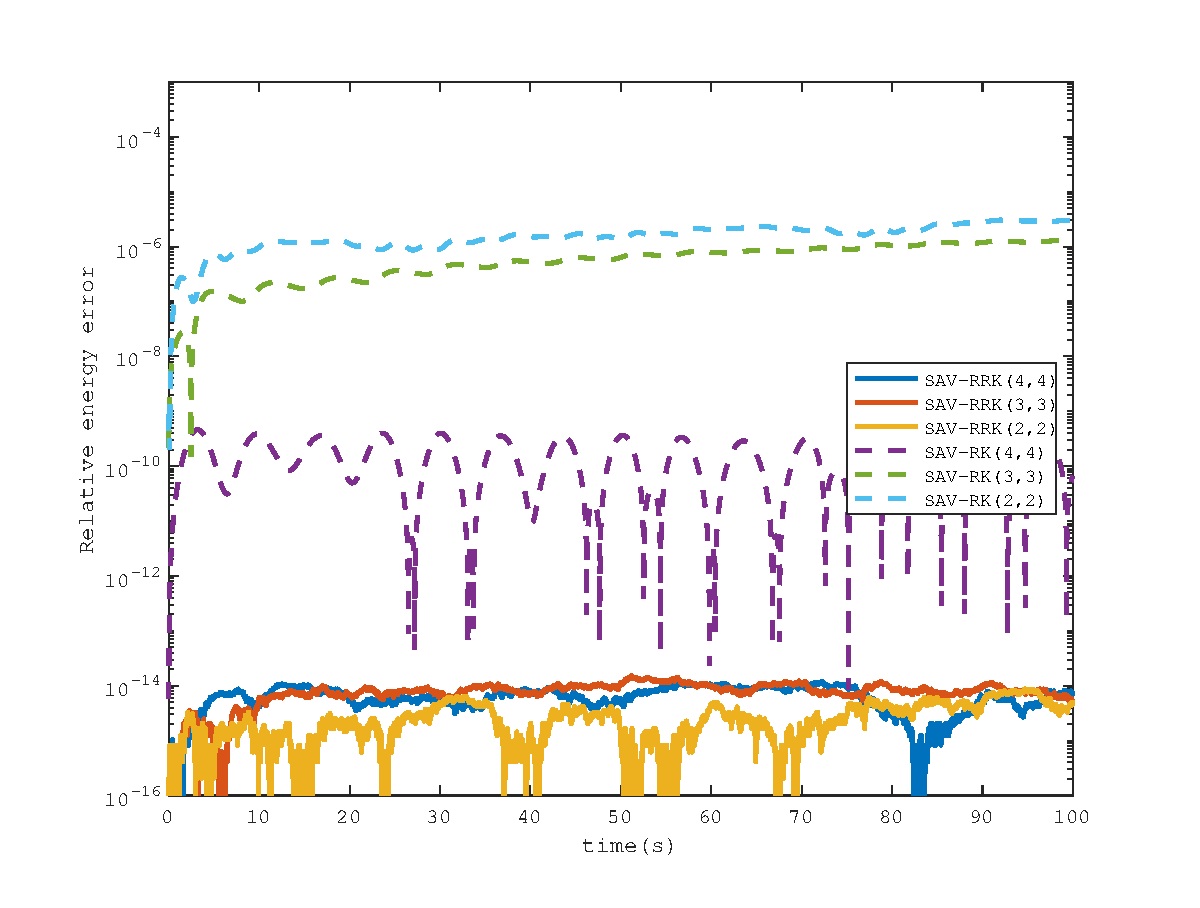
\includegraphics[width=0.5\textwidth]{./figures/exp4_energy6.eps}
		%\centerline{($a$) Temporal accuracy with $N=128.$}
		}\caption{当 $N=4, \tau=0.01$ 时,例 \ref{exp_SAVRRK:4} 中不同的 $\alpha$ 对应的相对能量误差.}
		\label{fig_SAVRRK:3-5}
		\end{center}
		\end{figure}
\end{frame}

\begin{frame}%\frametitle{数值算例}
	\begin{figure}[H]
		\begin{center}
		\subfigure[$\alpha,\beta=1.9$]{ \centering
		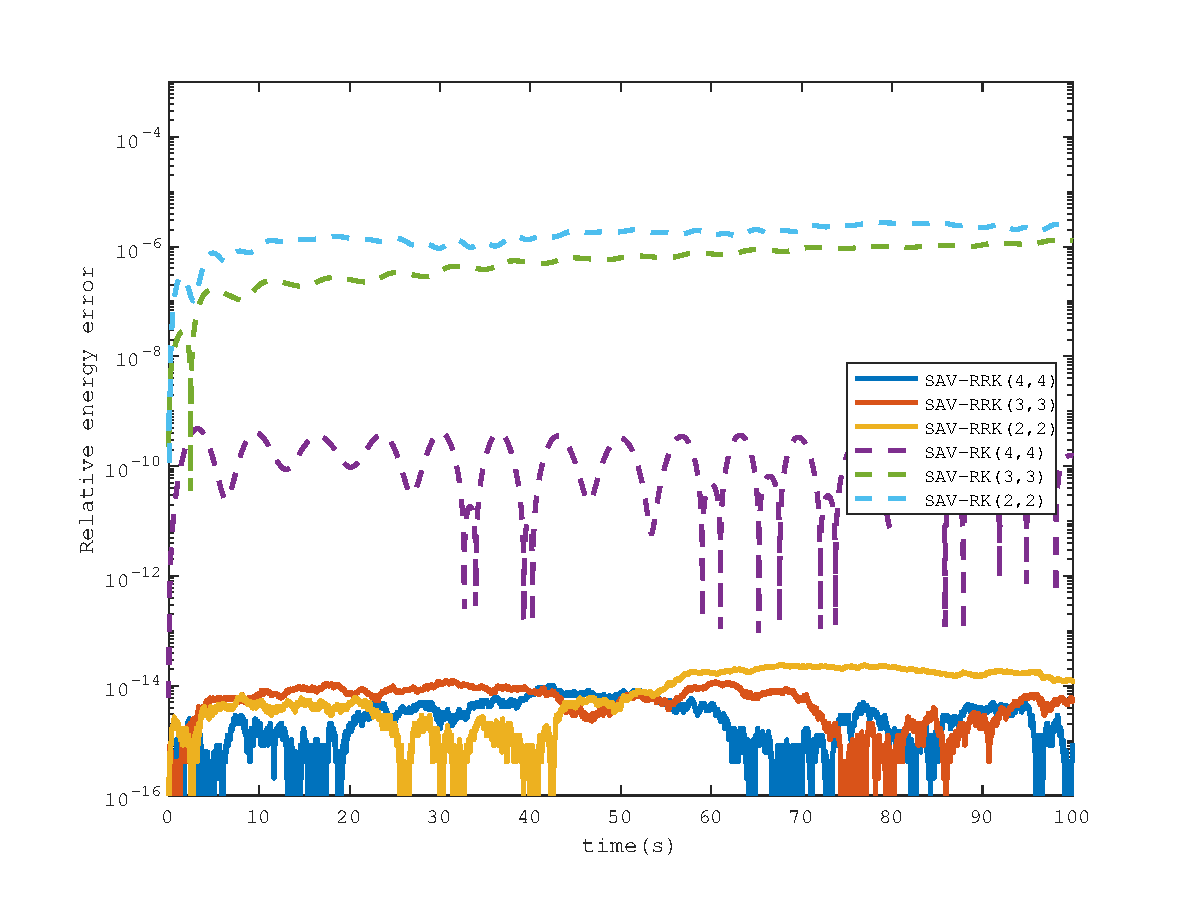
\includegraphics[width=0.5\textwidth]{./figures/exp4_energy9.eps}
		%\centerline{($b$) Spatial accuracy with $\tau = 10^{-3}.$}
		}\subfigure[$\alpha,\beta=2$]{ \centering
		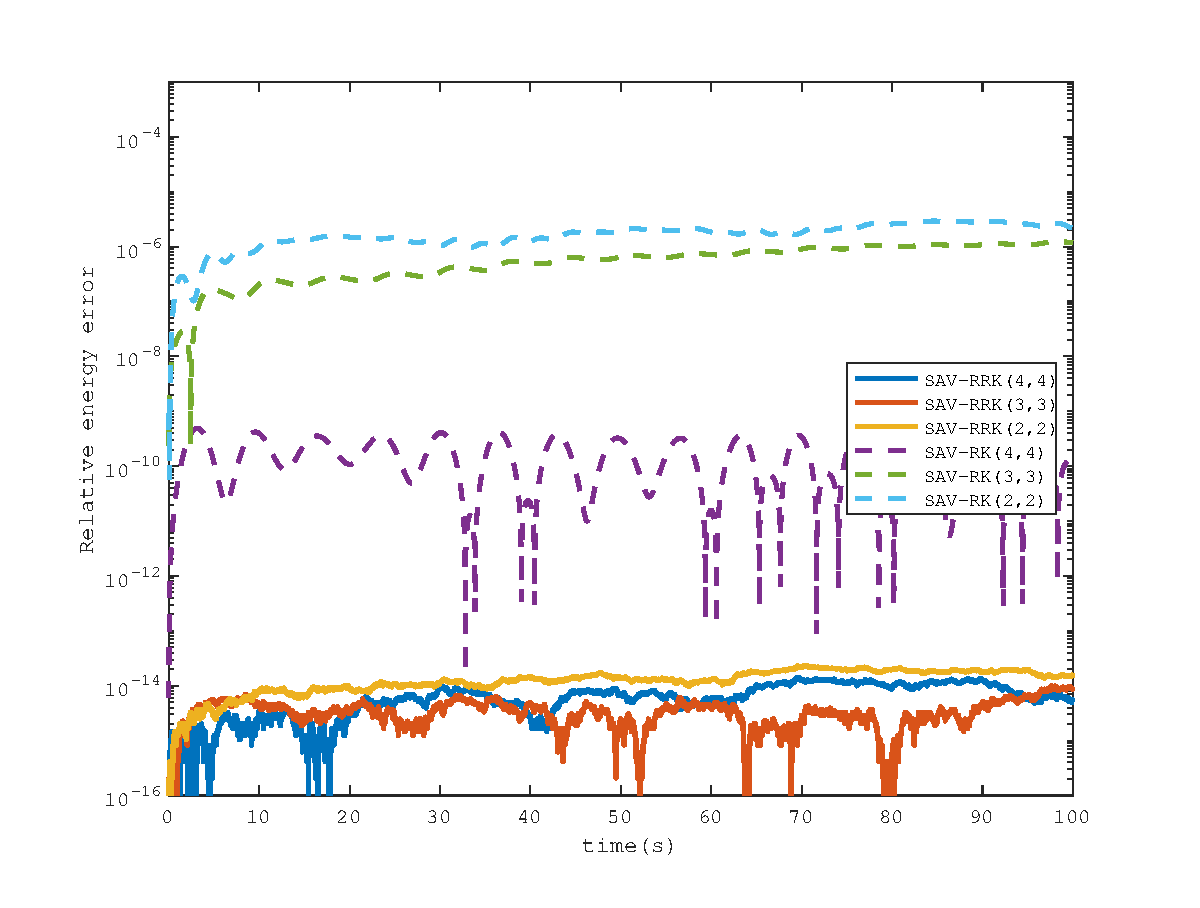
\includegraphics[width=0.5\textwidth]{./figures/exp4_energy2.eps}
		%\centerline{($a$) Temporal accuracy with $N=128.$}
		}
		% \caption{ Relative errors of energy with $N=4, \tau=0.01$ for different $\alpha$ in Example \ref{exp_SAVRRK:4}.}
		\caption{当 $N=4, \tau=0.01$ 时,例 \ref{exp_SAVRRK:4} 中不同的 $\alpha$ 对应的相对能量误差.}
		\label{fig_SAVRRK:3-5}
		\end{center}
		\end{figure}
\end{frame}

\begin{frame}\frametitle{小结}
	本章首先考虑了具有周期性边界条件的二维非线性分数阶薛定谔波方程,并通过标量辅助变量方法将其转化为一个等效系统,其中能量被重新表述为三个二次项的和.
	随后,结合显式松弛龙格库塔方法成功\textbf{\textcolor[rgb]{0.227,0.373,0.306}{构造了一个在时间方向可达任意高阶的显式保结构数值格式.}}
	最后,通过一系列数值实验验证了该格式在长时间仿真中的数值稳定性,并证明了所提方法对于其他类似的守恒问题也是有效的,
	如分数Klein-Gordon-Schr{\"o}dinger方程等.	
\end{frame}

\subsection{FPAVF-P算法}
\begin{frame}{研究内容及其可行性研究}
	\begin{block}{同时保持原始能量和原始质量守恒的数值格式}
		\textbf{\textcolor[rgb]{0.227,0.373,0.306}{研究内容:}}
		
		{\footnotesize 本课题首先通过分数阶Laplacian泛函的变分导数将NFSWEs重新表述为哈密顿系统.然后结合PAVF系列方法为二维NFSWEs构造能够同时保原始能量和原始质量的守恒格式.}
		
		\textbf{\textcolor[rgb]{0.227,0.373,0.306}{可行性分析:}}
		\begin{itemize}
			\item {\footnotesize PAVF方法可以守恒除常规能量之外的更多守恒性质,并已被用于构造哈密顿常微分方程的守恒格式\cite{caiPartitionedAveragedVector2018}.​​​​​​​​​​​​​​​​​​​​​​​​​​​​​​​​​​​​​​​​​​​​​​​​​​​​​​​​​​​​​​​​​​​​​​​​​​​​​​​​​​​​​​​​​​​​​​​​​​​​​​​​​​​​​​​​​​​​​​​​​​​​​​​​​​​​​​​​​​​​​​​​​​​​​​​​​​​​​​​​​​​​​​​​​​​​​​​​​​​​​​​​​​​​​​​​​​​​​​​​​​​​​​​​​​​​​​​​​​​​​​​​​​​​​​​​​​​​​​​​​​​​​​​​​​​​​​​​​​​​​​​​​​​​​​​​​​​​​​​​​​​​​​​​​​​​​​​​​​​​​​​​​​​​​​​​​​​​​​​​​​}
			\item {\footnotesize Wang 和 Huang \cite{wangStructurepreservingNumericalMethods2018} 提出了分数阶Laplacian泛函的变分导数并将一维分数阶非线性Schrödinger方程重新表述为哈密顿系统.Fu 和 Cai \cite{fuStructurepreservingAlgorithmsTwodimensional2020} 推导了二维分数阶 Klein-Gordon-Schrödinger 方程的哈密顿公式,并随后构建了守恒格式.}
			\end{itemize}
	\end{block}
	\end{frame}

\begin{frame}{NFSWEs的哈密顿格式构建}
	哈密顿结构对于构建PAVF格式至关重要.然而,目前没有研究人员考虑过带有周期边界条件的NFSWEs  的哈密顿结构.
	基于此, 本小节推导了 NFSWEs 的哈密顿结构.
	
	设
	\begin{align}
	u = p+\mathrm{i}q, \quad u_t = \varphi+ \mathrm{i}\psi,
	\end{align}
	其中$p, q,\varphi,\psi$均为实值函数.那么,NFSWEs  可以重写为
	\begin{align}\label{eq_PAVF:28}
	\varphi_{t}+\mathrm{i}\psi_{t}+\left( -\Delta \right) ^{\frac{\alpha }{2}}p+\mathrm{i}\left( -\Delta \right) ^{\frac{\alpha }{2}}q+\mathrm{i}\kappa \varphi-\kappa \psi+\beta \left( p^{2}+q^{2}\right) \left( p+\mathrm{i} q\right) =0.
	\end{align}
	\end{frame}

	\begin{frame}{NFSWEs的哈密顿格式构建}
		分离实部和虚部,得到
		\begin{align}
		&\varphi_{t}+\left( -\Delta \right) ^{\frac{\alpha }{2}}p-\kappa \psi+\beta \left( p^{2}+q^{2}\right)p=0,\nonumber\\
		&\psi_{t}+\left( -\Delta \right) ^{\frac{\alpha }{2}}q+\kappa \varphi+\beta \left( p^{2}+q^{2}\right)q=0.\label{eq_PAVF:29}
		\end{align}
		即,NFSWEs  可以重写为一个等效的耦合系统
		\begin{align}
		&\varphi_{t}=-\left( -\Delta \right) ^{\frac{\alpha }{2}}p+\kappa \psi-\beta \left( p^{2}+q^{2}\right)p\label{eq_PAVF:30},\\
		&\psi_{t}=-\left( -\Delta \right) ^{\frac{\alpha }{2}}q-\kappa \varphi-\beta \left( p^{2}+q^{2}\right)q\label{eq_PAVF:31},\\
		&p_t=\varphi, \label{eq_PAVF:32}\\
		&q_t=\psi, \label{eq_PAVF:33}
		\end{align}
		其中$p, q,\varphi,\psi$满足周期边界条件.
	\end{frame}
\begin{frame}%{NFSWEs的哈密顿格式构建}
	% 为了得到NFSWEs  的哈密顿形式,引入以下两个重要引理.
	\begin{lemma}\label{lem_PAVF:1}
		\cite{fuStructurepreservingAlgorithmsTwodimensional2020} 
		 给定 $1<\alpha \leq 2$,那么对于任何实值周期函数 $p, q \in L^{2}(\Omega)$,有
		\begin{align}\label{eq_PAVF:22}
		\int_{\Omega}(-\Delta)^{\frac{\alpha}{2}} p q d \boldsymbol{x}=\int_{\Omega}(-\Delta)^{\frac{\alpha}{4}} p(-\Delta)^{\frac{\alpha}{4}} q d \boldsymbol{x}=\int_{\Omega} p(-\Delta)^{\frac{\alpha}{2}} q d \boldsymbol{x}.
		\end{align}
		\end{lemma}
		
\begin{lemma}\label{lem_PAVF:2}
	\cite{wangStructurepreservingNumericalMethods2018} 
	 对于形如
	\begin{align}\label{eq_PAVF:25}
	F[g]=\int_{\Omega} f\left(g(\boldsymbol{x}),(-\Delta)^{\frac{\alpha}{4}} g(\boldsymbol{x})\right) d \boldsymbol{x},
	\end{align}
	的泛函 $F[g]$, $f$ 是 $\Omega$ 上的光滑函数,其变分导数如下
	\begin{align}\label{eq_PAVF:26}
	\frac{\delta F}{\delta g}=\frac{\partial f}{\partial g}+(-\Delta)^{\frac{\alpha}{4}} \frac{\partial f}{\partial\left((-\Delta)^{\frac{\alpha}{4}} g\right)} .
	\end{align}
	\end{lemma}
	\end{frame}


\begin{frame}{NFSWEs的哈密顿格式构建}
	基于上述引理,可以得到以下结果.

	\begin{theorem}	\label{thm_PAVF:2_1}
	设
	\begin{align}
	&\mathcal{G}=\kappa\int_{\Omega}(p^2+q^2) d \boldsymbol{x}+2\operatorname{Im}(\int_{\Omega}(\varphi+\mathrm{i}\psi)(p-\mathrm{i}q)d \boldsymbol{x}),\label{eq_PAVF:34} \\
	&\mathcal{H}=\frac{1}{2}\int_{\Omega}\left((\varphi^2+\psi^2)+\left((-\Delta)^{\frac{\alpha}{4}} p\right)^{2}+\left((-\Delta)^{\frac{\alpha}{4}} q\right)^{2}+\frac{\beta}{2}(p^2+q^2)^{2}\right) d \boldsymbol{x}.\label{eq_PAVF:35}
	\end{align}
	那么等效系统 \eqref{eq_PAVF:30}-\eqref{eq_PAVF:33} 具有以下两个守恒定律:
	\begin{align}
	\frac{d}{d t} \mathcal{G}=0, \quad \frac{d}{d t} \mathcal{H}=0.
	\end{align}
	\end{theorem}
\end{frame}


\begin{frame}{NFSWEs的哈密顿格式构建}

	\begin{theorem}\label{thm_PAVF:2}
		NFSWEs 可以被重构为以下哈密顿系统:
	\begin{equation}\label{eq_PAVF:37}
		\left(\begin{array}{l}
			\varphi_{t} \\
			\psi_{t} \\
			p_{t} \\
			q_{t}
			\end{array}\right)=J\left(\begin{array}{l}
			\delta \mathcal{H} / \delta \varphi \\
			\delta \mathcal{H} / \delta \psi \\
			\delta \mathcal{H} / \delta p \\
			\delta \mathcal{H} / \delta q
			\end{array}\right),
	\end{equation}
	其中 哈密顿 算符
	\begin{equation}\label{eq_PAVF:37b}
	J=\left(\begin{array}{cccc}
			0 & \kappa & -1 & 0 \\
			-\kappa & 0 & 0 & -1 \\
			1 & 0 & 0 & 0 \\
			0 & 1 & 0 & 0
			\end{array}\right),
	\end{equation}
	能量泛函 $\mathcal{H}$ 定义如 \eqref{eq_PAVF:35}.
	\end{theorem}
\end{frame}

\begin{frame}{傅里叶拟谱离散格式}
	鉴于周期性边界条件,选择傅里叶拟谱法离散等效系统 \eqref{eq_PAVF:30}-\eqref{eq_PAVF:33},
	得到如下的空间半离散系统:
	\begin{align}
	&\varPhi_{t}=D^{\alpha}P+\kappa \Psi-\beta \left( P^{2}+Q^{2}\right)\cdot P,\label{eq_PAVF:56}\\
	&\Psi_{t}=D^{\alpha}Q-\kappa \varPhi-\beta \left( P^{2}+Q^{2}\right)\cdot Q,\label{eq_PAVF:57}\\
	&P_t=\varPhi,\label{eq_PAVF:58}\\
	&Q_t=\Psi,\label{eq_PAVF:59}
	\end{align}
	其中$P^{2}=P \cdot P$,而 $\cdot$表示向量之间的点乘.
	简洁起见,定义向量
\begin{align}\label{eq_PAVF:60a}
Y=\left(\varPhi^{T}, \Psi^{T}, P^{T}, Q^{T}\right),
\end{align}
\end{frame}
\begin{frame}{傅里叶拟谱离散格式}
	上述半离散系统可重新表示哈密顿形式
	\begin{align}\label{eq_PAVF:60}
	\frac{d Y}{d t}=f(Y)=S \nabla H(Y),
	\end{align}
	哈密顿能量定义如下
	\begin{align}\label{eq_PAVF:61}
		H(Y)=\frac{1}{2}\left((\varPhi^{T}\varPhi+\Psi^{T}\Psi){-P^{T} D^{\alpha} P-Q^{T} D^{\alpha} Q}+\frac{\beta}{2}(P^2+Q^2)^{T}(P^2+Q^2)\right),
	\end{align}
	其中$S$是具有以下形式的反对称矩阵
	\begin{align}\label{eq_PAVF:62}
	S=\left(\begin{array}{cccc}
	0 & \kappa I & -I & 0 \\
	-\kappa I & 0 & 0 & -I \\
	I & 0 & 0 & 0 \\
	0 & I & 0 & 0
	\end{array}\right).
	\end{align}
	
\end{frame}
\begin{frame}{傅里叶拟谱离散格式}
	此外,定义质量
	\begin{align}\label{eq_PAVF:63}
	G(Y)=\kappa\|P\|^{2}+\kappa\|Q\|^{2} +2\Psi^{T}P-2\varPhi^{T}Q.
	\end{align}
	
\begin{theorem}	\label{thm_PAVF:3}
	半离散系统 \eqref{eq_PAVF:56}-\eqref{eq_PAVF:59} 具有质量和能量守恒定律:
\begin{align}
\frac{d G(Y)}{d t}=0,~\frac{d H(Y)}{d t}=0.
\end{align}
\end{theorem} 
\end{frame}

\begin{frame}{FPAVF-P格式}
	对哈密顿系统\eqref{eq_PAVF:60}应用PAVF方法:
	\begin{align}
	\delta_{t} \varPhi^{m}=&\int_{0}^{1}\kappa H_{\Psi}\left(\varPhi^{m+1}, \varepsilon \Psi^{m+1}+(1-\varepsilon) \Psi^{m}, P^{m}, Q^{m}\right)d \varepsilon\nonumber\\
	&-\int_{0}^{1}H_{P}\left(\varPhi^{m+1}, \Psi^{m+1}, \varepsilon P^{m+1}+(1-\varepsilon) P^{m}, Q^{m}\right)d \varepsilon,\label{eq_PAVF:70}\\
	\delta_{t} \Psi^{m}=&-\int_{0}^{1}\kappa H_{\varPhi}\left(\varepsilon \varPhi^{m+1}+(1-\varepsilon) \varPhi^{m}, \Psi^{m}, P^{m}, Q^{m}\right)d \varepsilon\nonumber\\
	&+\int_{0}^{1}H_{Q}\left(\varPhi^{m+1}, \Psi^{m+1}, P^{m+1}, \varepsilon Q^{m+1}+(1-\varepsilon) Q^{m}\right)d\varepsilon,\label{eq_PAVF:71}\\
	\delta_{t} P^{m}=&\int_{0}^{1}H_{\varPhi}\left(\varepsilon \varPhi^{m+1}+(1-\varepsilon) \varPhi^{m}, \Psi^{m}, P^{m}, Q^{m}\right) d \varepsilon,\label{eq_PAVF:72}\\
	\delta_{t} Q^{m}=&\int_{0}^{1}H_{\Psi}\left(\varPhi^{m+1}, \varepsilon \Psi^{m+1}+(1-\varepsilon) \Psi^{m}, P^{m}, Q^{m}\right) d \varepsilon.\label{eq_PAVF:73}
	\end{align}
\end{frame}

\begin{frame}{FPAVF-P格式}
	上述数值格式可以进一步整合为如下傅里叶拟谱 PAVF(FPAVF)格式:
	\begin{align}
	\delta_{t} \varPhi^{m}=&~\kappa \Psi^{m+\frac{1}{2}}{+D^{\alpha} P^{m+\frac{1}{2}}}-\frac{\beta}{4}\left( (P^{m+1})^3+ (P^{m})^{2}\cdot P^{m+1}+(P^{m+1})^{2}\cdot P^{m}\right.\nonumber\\
		&+\left. (P^{m})^{3}+2 P^{m+1}\cdot (Q^{m})^{2}+2 P^{m}\cdot (Q^{m})^{2}\right),\label{eq_PAVF:74}\\
	\delta_{t} \Psi^{m}=&-\kappa \varPhi^{m+\frac{1}{2}}{+D^{\alpha} Q^{m+\frac{1}{2}}}-\frac{\beta}{4}\left( (Q^{m+1})^3+ (Q^{m})^{2}\cdot Q^{m+1}+(Q^{m+1})^{2}\cdot Q^{m}\right.\nonumber\\
		&+\left. (Q^{m})^{3}+2 Q^{m+1}\cdot (P^{m+1})^{2}+2 Q^{m}\cdot (P^{m+1})^{2}\right),\label{eq_PAVF:75}\\
	\delta_{t} P^{m}=&~\varPhi^{m+\frac{1}{2}},\label{eq_PAVF:76}\\
	\delta_{t} Q^{m}=&~\Psi^{m+\frac{1}{2}}.\label{eq_PAVF:77}
	\end{align}
	FPAVF并不能保证质量守恒, 这可以在数值算例中被反映出来.
\end{frame}

\begin{frame}{FPAVF-P格式}
	FPAVF格式\eqref{eq_PAVF:74}-\eqref{eq_PAVF:77}的伴随格式为
	\begin{align}
	\delta_{t} \varPhi^{m}=&~\kappa \Psi^{m+\frac{1}{2}}{+D^{\alpha} P^{m+\frac{1}{2}}}-\frac{\beta}{4}\left( (P^{m+1})^3+ (P^{m})^{2}\cdot P^{m+1}+(P^{m+1})^{2}\cdot P^{m}\right.\nonumber\\
		&\left.+ (P^{m})^{3}+2 P^{m+1}\cdot (Q^{m+1})^{2}+2 P^{m}\cdot (Q^{m+1})^{2}\right),\label{eq_PAVF:86}\\
	\delta_{t} \Psi^{m}=&-\kappa \varPhi^{m+\frac{1}{2}}{+D^{\alpha} Q^{m+\frac{1}{2}}}-\frac{\beta}{4}\left( (Q^{m+1})^3+ (Q^{m})^{2}\cdot Q^{m+1}+ (Q^{m+1})^{2}\cdot Q^{m}\right.\nonumber\\
		&\left.+ (Q^{m})^{3}+2 Q^{m+1}\cdot (P^{m})^{2}+2 Q^{m}\cdot (P^{m})^{2}\right),\label{eq_PAVF:87}\\
	\delta_{t} P^{m}=&~\varPhi^{m+\frac{1}{2}},\label{eq_PAVF:88}\\
	\delta_{t} Q^{m}=&~\Psi^{m+\frac{1}{2}}.\label{eq_PAVF:89}
	\end{align}
	
\end{frame}
\begin{frame}{FPAVF-P格式}
	将FPAVF格式\eqref{eq_PAVF:74}-\eqref{eq_PAVF:77}与其伴随FPAVF格式\eqref{eq_PAVF:86}-\eqref{eq_PAVF:89}相结合,得到傅里叶 拟谱 PAVF-P(FPAVF-P)格式如下:
	\begin{align}
	\delta_{t} \varPhi^{m}=&~\kappa \Psi^{m+\frac{1}{2}}{+D^{\alpha} P^{m+\frac{1}{2}}}-\frac{\beta}{4}\left((P^{m+1})^3+(P^{m})^{2}\cdot P^{m+1}+(P^{m+1})^{2}\cdot P^{m}\right.\nonumber\\
		&\left.+(P^{m})^{3}+P^{m+1}\cdot (Q^{m})^{2}+P^{m}\cdot (Q^{m})^{2}+P^{m+1}\cdot (Q^{m+1})^{2}+P^{m}\cdot (Q^{m+1})^{2}\right),\label{eq_PAVF:98}\\
	\delta_{t} \Psi^{m}=&-\kappa \varPhi^{m+\frac{1}{2}}{+D^{\alpha} Q^{m+\frac{1}{2}}}-\frac{\beta}{4}\left((Q^{m+1})^3+(Q^{m})^{2}\cdot Q^{m+1}+(Q^{m+1})^{2}\cdot Q^{m}\right.\nonumber\\
		&\left.+(Q^{m})^{3}+Q^{m+1}\cdot (P^{m+1})^{2}+Q^{m}\cdot (P^{m+1})^{2}+Q^{m+1}\cdot (P^{m})^{2}+Q^{m}\cdot (P^{m})^{2}\right),\label{eq_PAVF:99}\\
	\delta_{t} P^{m}=&~\varPhi^{m+\frac{1}{2}},\label{eq_PAVF:100}\\
	\delta_{t} Q^{m}=&~\Psi^{m+\frac{1}{2}}.\label{eq_PAVF:101}
	\end{align}
	
\end{frame}
\begin{frame}{离散守恒律}
	\begin{theorem}\label{thm_PAVF:4}
		FPAVF-P格式\eqref{eq_PAVF:98}-\eqref{eq_PAVF:101}在离散意义上具有以下能量守恒和质量守恒的特性:
		\begin{align}\label{eq_PAVF:11141}
		G^{m+1}=G^{m}, \quad H^{m+1}=H^{m}, \quad 0 \leq m \leq M-1,
		\end{align}
		其中离散质量为
		\begin{align}\label{eq_PAVF:11142}
		G^{m}=\kappa\|P^{m}\|^2+\kappa\|Q^{m}\|^2+2 \left(\Psi^{m}\right)^T P^{m}-2 \left(\varPhi^{m}\right)^T Q^{m},
		\end{align}
		离散能量为
		\begin{align}
		H^{m}=&\frac{1}{2}[((\varPhi^{m})^{T}\varPhi^{m}+(\Psi^{m})^{T}\Psi^{m}){-(P^{m})^{T} D^{\alpha} P^{m}-(Q^{m})^{T} D^{\alpha} Q^{m}}\nonumber\\
		&+\frac{\beta}{2}((P^{m})^2+(Q^{m})^2)^{T}((P^{m})^2+(Q^{m})^2)].\label{eq_PAVF:800}
		\end{align}
		\end{theorem}
\end{frame}
\begin{frame}{其他数值方法}
	FAVF(傅里叶拟谱AVF)格式
	\begin{align}
	\delta_{t} \varPhi =&~{D^{\alpha} P^{m+\frac{1}{2}}}+\kappa \Psi^{m+\frac{1}{2}}-\frac{\beta}{12}\left(3 (P^{m+1})^3-5 (P^{m+1})^2\cdot P^{m}\right.\nonumber\\
			&-5 (P^{m})^2\cdot P^{m+1}+19 (P^{m})^3-6 Q^{m+1}\cdot Q^{m}\cdot P^{m}+2 Q^{m+1}\cdot Q^{m}\cdot P^{m+1} \nonumber\\
			&+\left. 3 (Q^{m+1})^2\cdot P^{m+1}+(Q^{m})^2\cdot P^{m+1}-7 (Q^{m+1})^2\cdot P^{m}+19 (Q^{m} )^2\cdot P^{m}\right),\label{eq_PAVF:66}\\
	\delta_{t} \Psi =&~{D^{\alpha} Q^{m+\frac{1}{2}}}-\kappa \varPhi^{m+\frac{1}{2}}-\frac{\beta}{12}\left(3 (Q^{m+1})^3-5 (Q^{m+1})^2\cdot Q^{m}\right.\nonumber\\
			&-5 (Q^{m})^2\cdot Q^{m+1}+19 (Q^{m})^3-6 P^{m+1}\cdot P^{m}\cdot Q^{m}+2 P^{m+1}\cdot P^{m}\cdot Q^{m+1} \nonumber\\
			&+\left. 3 (P^{m+1})^2\cdot Q^{m+1}+(P^{m})^2\cdot Q^{m+1}-7 (P^{m+1})^2\cdot Q^{m}+19 (P^{m} )^2\cdot Q^{m}\right),\label{eq_PAVF:67}\\
	\delta_{t} P=&~\varPhi^{m+\frac{1}{2}},\label{eq_PAVF:68}\\
	\delta_{t} Q=&~\Psi^{m+\frac{1}{2}}.\label{eq_PAVF:69}
	\end{align}
\end{frame}
\begin{frame}{其他数值方法}
	FPAVF-C(傅里叶拟谱PAVF组合)格式
	\begin{align}
	&\frac{1}{\tau}\left(\varPhi^{*}-\varPhi^{m}\right)=\frac{1}{2}\kappa(\Psi^{*}+\Psi^{m}){+\frac{1}{2}D^{\alpha} (P^{*}+P^{m})}-\frac{\beta}{4}\left( (P^{*})^3+ (P^{m})^{2}\cdot P^{*}\right.\nonumber\\
			&~~~~~~~~~~~~~~~~~~~~\left.+ (P^{*})^{2}\cdot P^{m}+ (P^{m})^{3}+2 P^{*}\cdot (Q^{m})^{2}+2 P^{m}\cdot (Q^{m})^{2}\right),\label{eq_PAVF:90}\\
	&\frac{1}{\tau}\left(\Psi^{*}-\Psi^{m}\right)=-\frac{1}{2}\kappa (\varPhi^{*}+\varPhi^{m}){+\frac{1}{2}D^{\alpha} (Q^{*}+Q^{m})}-\frac{\beta}{4}\left( (Q^{*})^3+ (Q^{m})^{2}\cdot Q^{*}\right.\nonumber\\
			&~~~~~~~~~~~~~~~~~~~~~\left.+ (Q^{*})^{2}\cdot Q^{m}+ (Q^{m})^{3}+2 Q^{*}\cdot (P^{*})^{2}+2 Q^{m}\cdot (P^{*})^{2}\right),\label{eq_PAVF:91}\\
	&\frac{1}{\tau}\left(P^{*}-P^{m}\right)=\frac{1}{2}(\varPhi^{*}+\varPhi^{m}),\label{eq_PAVF:92}\\
	&\frac{1}{\tau}\left(Q^{*}-Q^{m}\right)=\frac{1}{2}(\Psi^{*}+\Psi^{m}),\label{eq_PAVF:93}\\
	\end{align}
\end{frame}

\begin{frame}{其他数值方法}
	FPAVF-C(傅里叶拟谱PAVF组合)格式
	\begin{align}
	&\frac{1}{\tau}\left(\varPhi^{m+1}-\varPhi^{*}\right)=\frac{1}{2}\kappa (\Psi^{m+1}+\Psi^{*}){+\frac{1}{2}D^{\alpha} P^{m+\frac{1}{2}}}-\frac{\beta}{4}\left((P^{m+1})^3+(P^{*})^{2}\cdot P^{m+1}\right.\nonumber\\
			&~~~~~~~~~~~~~~~~~~~~~~~\left.+(P^{m+1})^{2}\cdot P^{*}+ (P^{*})^{3}+2 P^{m+1}\cdot (Q^{m+1})^{2}+2 P^{*}\cdot (Q^{m+1})^{2}\right),\label{eq_PAVF:94}\\
	&\frac{1}{\tau}\left(\Psi^{m+1}-\Psi^{*}\right)=-\frac{1}{2}\kappa (\varPhi^{m+1}+\varPhi^{*}){+\frac{1}{2}D^{\alpha} Q^{m+\frac{1}{2}}}-\frac{\beta}{4}\left((Q^{m+1})^3+(Q^{*})^{2}\cdot Q^{m+1}\right.\nonumber\\
			&~~~~~~~~~~~~~~~~~~~~~~~~\left.+(Q^{m+1})^{2}\cdot Q^{*}+ (Q^{*})^{3}+2 Q^{m+1}\cdot (P^{*})^{2}+2 Q^{*}\cdot (P^{*})^{2}\right),\label{eq_PAVF:95}\\
	&\frac{1}{\tau}\left(P^{m+1}-P^{*}\right)=\frac{1}{2}(\varPhi^{m+1}+\varPhi^{*}),\label{eq_PAVF:96}\\
	&\frac{1}{\tau}\left(Q^{m+1}-Q^{*}\right)=\frac{1}{2}(\Psi^{m+1}+\Psi^{*}),\label{eq_PAVF:97}
	\end{align}
	其中$\Phi^*, \Psi^*, P^*, Q^*$可以理解为从前一层迭代得到的中间变量,可作为计算后续层变量的输入.
\end{frame}
\begin{frame}{其他数值方法}

	\begin{remark}\label{rk_PAVF:1}
		类似于FPAVF-P格式\eqref{eq_PAVF:98}-\eqref{eq_PAVF:101},容易证明上述FPAVF格式\eqref{eq_PAVF:74}-\eqref{eq_PAVF:77}、FAVF格式\eqref{eq_PAVF:66}-\eqref{eq_PAVF:69}和FPAVF-C格式\eqref{eq_PAVF:90}-\eqref{eq_PAVF:97}均在离散意义上保证原始能量守恒,但不保证原始质量守恒.离散能量的形式与\eqref{eq_PAVF:800}中定义的相同.
		\end{remark}
		
		\begin{remark}\label{rk_PAVF:2}
		值得强调的是,用于求解NFSWEs  的其他现有方法仅保持修正后的能量和(或)修正后的质量.
		例如SAV方法 \cite{chengConvergenceEnergyconservingScheme2022}仅保持修正后的能量,
		三层线性隐式差分格式\cite{ranLinearlyImplicitConservative2016}保持修正后的能量和质量.
		然而,所提出的FPAVF-P格式\eqref{eq_PAVF:98}-\eqref{eq_PAVF:101}在离散意义上同时保持原始质量和能量, 这是本文的主要贡献之一.
		此外,FPAVF-P格式\eqref{eq_PAVF:98}-\eqref{eq_PAVF:101}在时间方向具有二阶精度,在空间方向具有谱精度.
		\end{remark}
\end{frame}

\begin{frame}{数值算例}
	\begin{example}\label{exp_PAVF:2}
		考虑一维非线性分数阶波动方程 ,具体形式为
		\begin{equation}\label{eq_PAVF:108}
		u_{t t}+(-\Delta)^{\alpha / 2} u+\mathrm{i}u_t+|u|^2 u=0, \quad (x,t)\in  \Omega\times[0, T],
		\end{equation}
		初值条件为 $u(x, 0)=(1+\mathrm{i}) x e^{-10(1-x)^2}$ 以及 $u_t(x, 0)=0$.
	\end{example}
\end{frame}

\begin{frame}%{数值算例}

	\begin{figure}[H]
		\begin{center}
		\subfigure[$\tau=1/1000$]{ \centering
		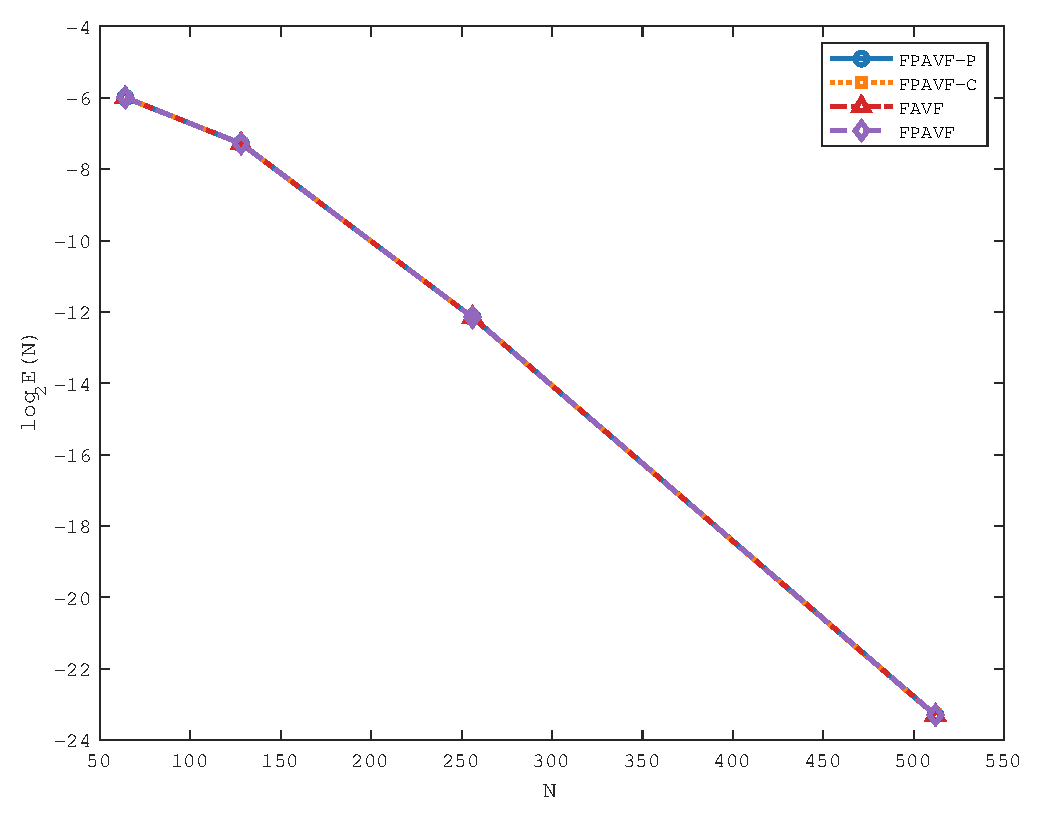
\includegraphics[width=0.5\textwidth]{./figure/exp1_s1.5.eps}
		%\centerline{($b$) Spatial accuracy with $\tau = 10^{-3}.$}
		}\subfigure[$N=128$]{ \centering
		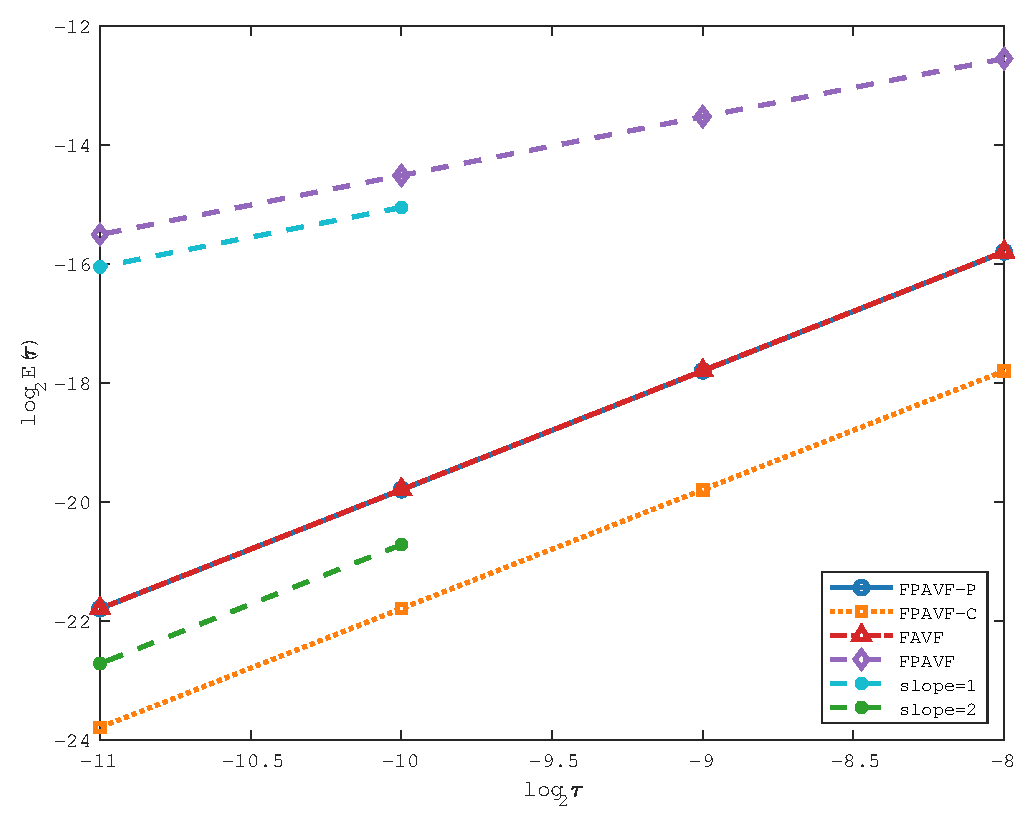
\includegraphics[width=0.5\textwidth]{./figure/exp1_t1.5.eps}
		%\centerline{($a$) Temporal accuracy with $N=128.$}
		}
		% \caption{Convergence orders of four schemes for Example \ref{exp_PAVF:2} with $\alpha=1.5$.}
		\caption{当$\alpha=1.5$时,例 \ref{exp_PAVF:2} 中四种格式的收敛阶.}
		 \label{fig_PAVF:1}
		\end{center}
		\end{figure}
\end{frame}

\begin{frame}%{数值算例}
	\begin{figure}[H]
		\begin{center}
		\subfigure[$\tau=1/1000$]{ \centering
		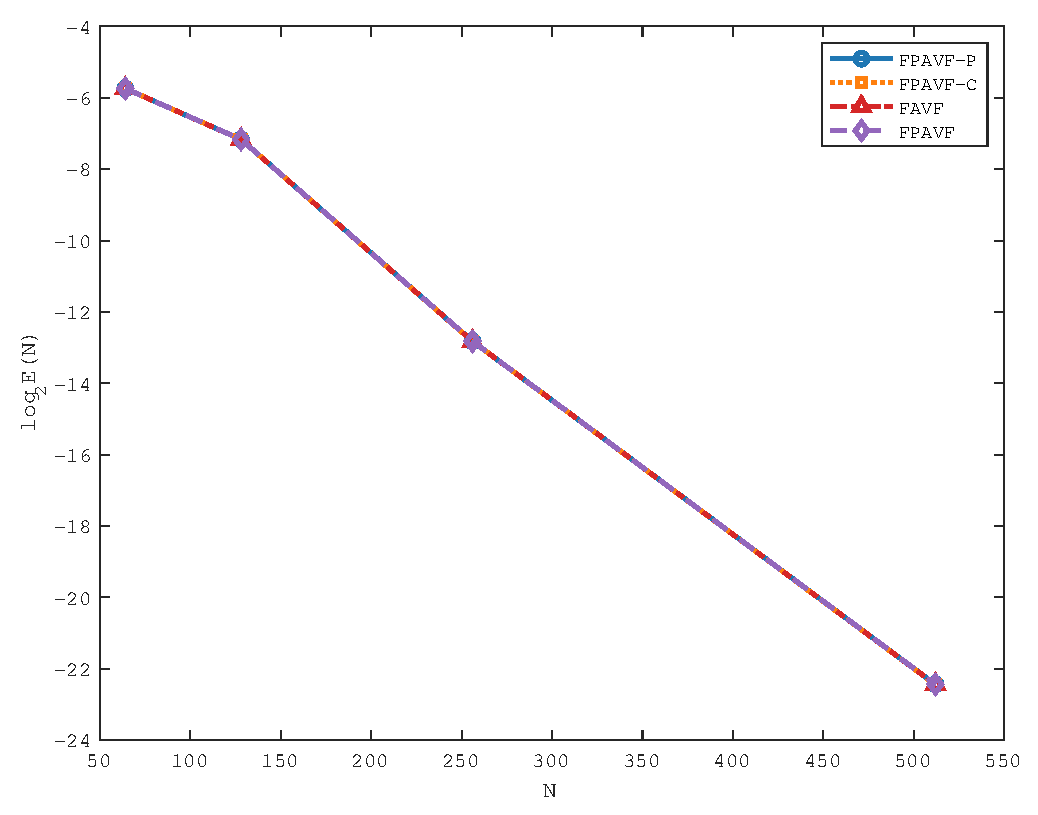
\includegraphics[width=0.5\textwidth]{./figure/exp1_s2.eps}
		%\centerline{($b$) Spatial accuracy with $\tau = 10^{-3}.$}
		}\subfigure[$N=128$]{ \centering
		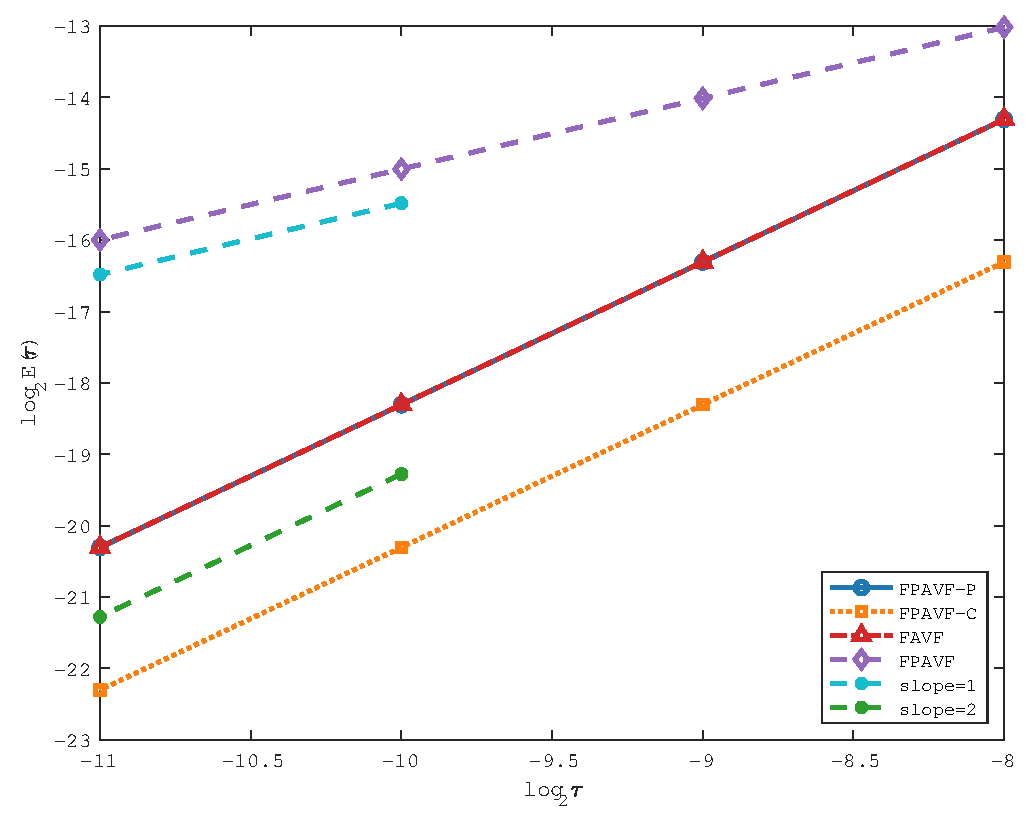
\includegraphics[width=0.5\textwidth]{./figure/exp1_t2.eps}
		%\centerline{($a$) Temporal accuracy with $N=128.$}
		}
		\caption{当$\alpha=2.0$时,例 \ref{exp_PAVF:2} 中四种格式的收敛阶.}
		% \caption{Convergence orders of four schemes for Example \ref{exp_PAVF:2} with $\alpha=2.0$.} 
		\label{fig_PAVF:2}
		\end{center}
		\end{figure}
\end{frame}

\begin{frame}%{数值算例}
	\begin{figure}[H]
		\begin{center}
		\subfigure[$\alpha=1.3$]{ \centering
		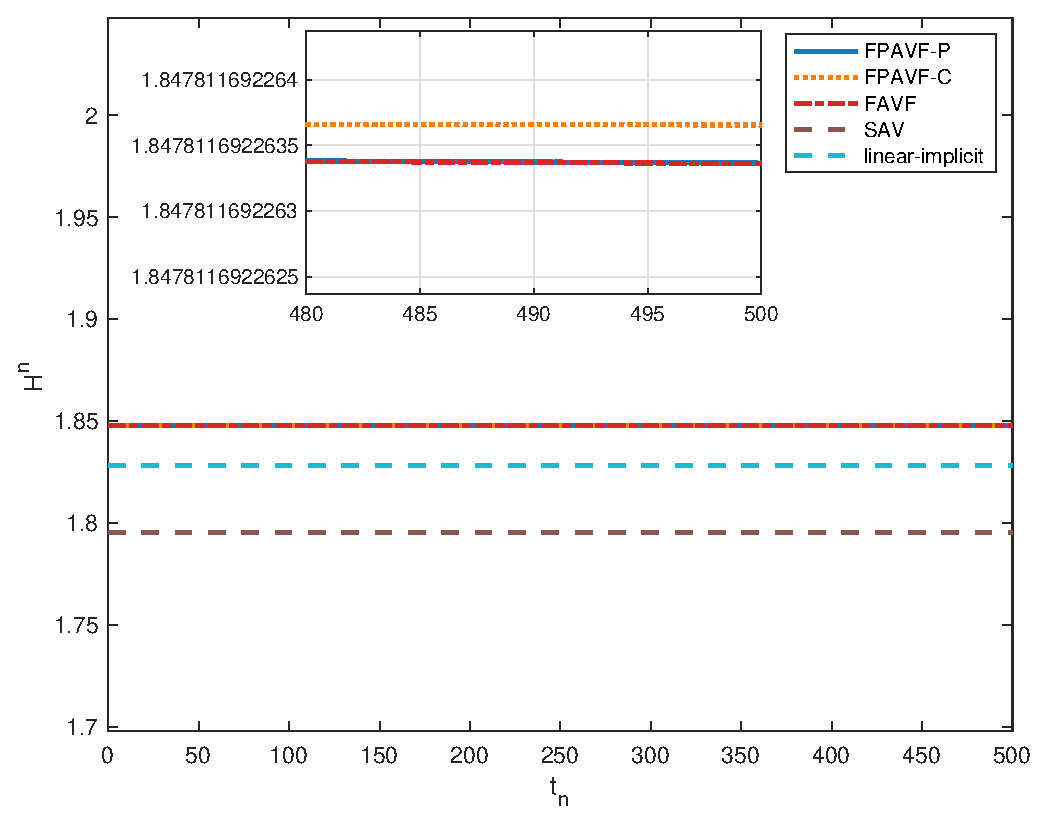
\includegraphics[width=0.5\textwidth]{./figure/exp1_H1.3.eps}
		%\centerline{($a$) $\alpha=1.3$}
		}\subfigure[$\alpha=1.6$]{ \centering
		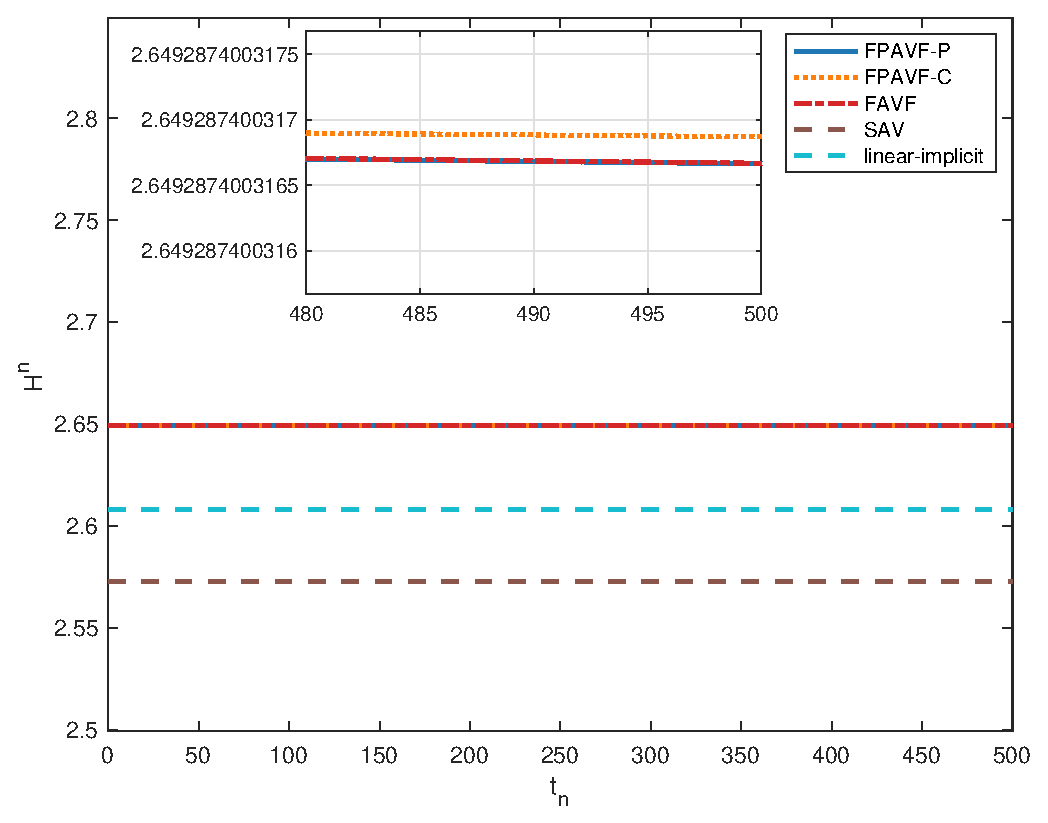
\includegraphics[width=0.5\textwidth]{./figure/exp1_H1.6.eps}
		%\centerline{($b$) $\alpha=1.6$}
		}\caption{在例 \ref{exp_PAVF:2} 中,当 $N = 512$ 且 $\tau=0.01$ 时,不同 $\alpha$ 下的离散能量.}
		\label{fig_PAVF:3}
		\end{center}
		\end{figure}
\end{frame}

\begin{frame}%{数值算例}
	\begin{figure}[H]
		\begin{center}
		\subfigure[$\alpha=1.9$]{ \centering
		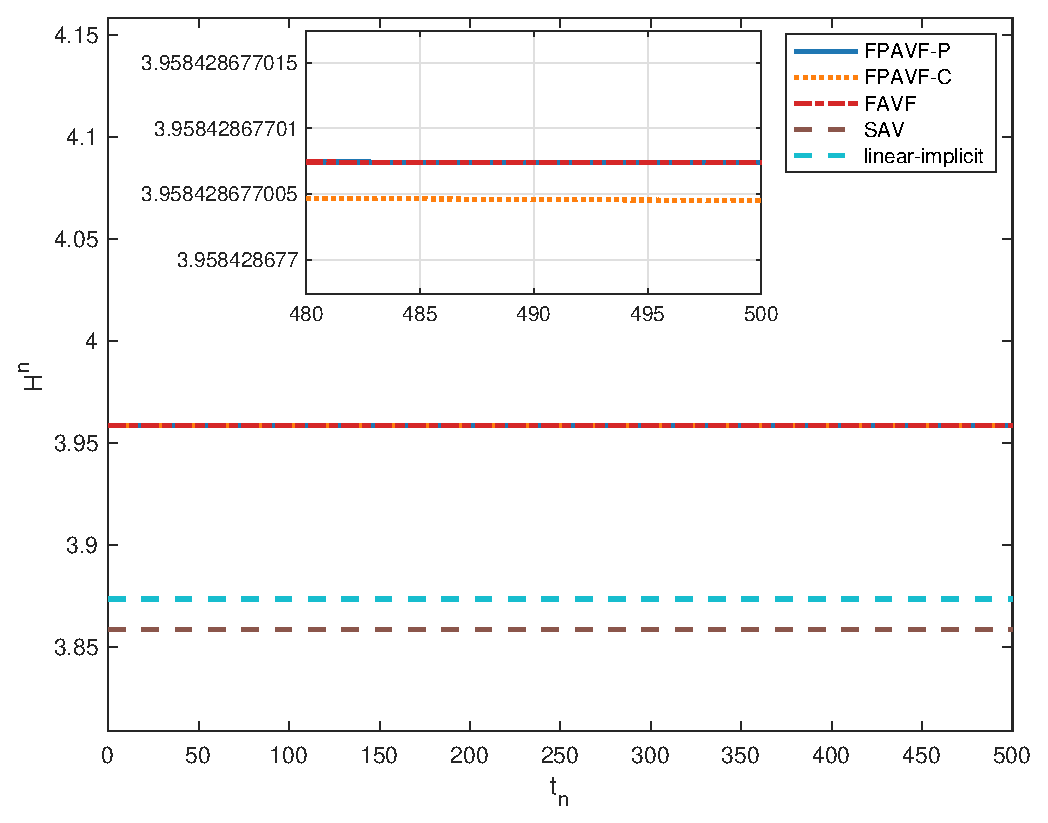
\includegraphics[width=0.5\textwidth]{./figure/exp1_H1.9.eps}
		%\centerline{($d$) $\alpha=2.0$}
		}\subfigure[$\alpha=2.0$]{ \centering
		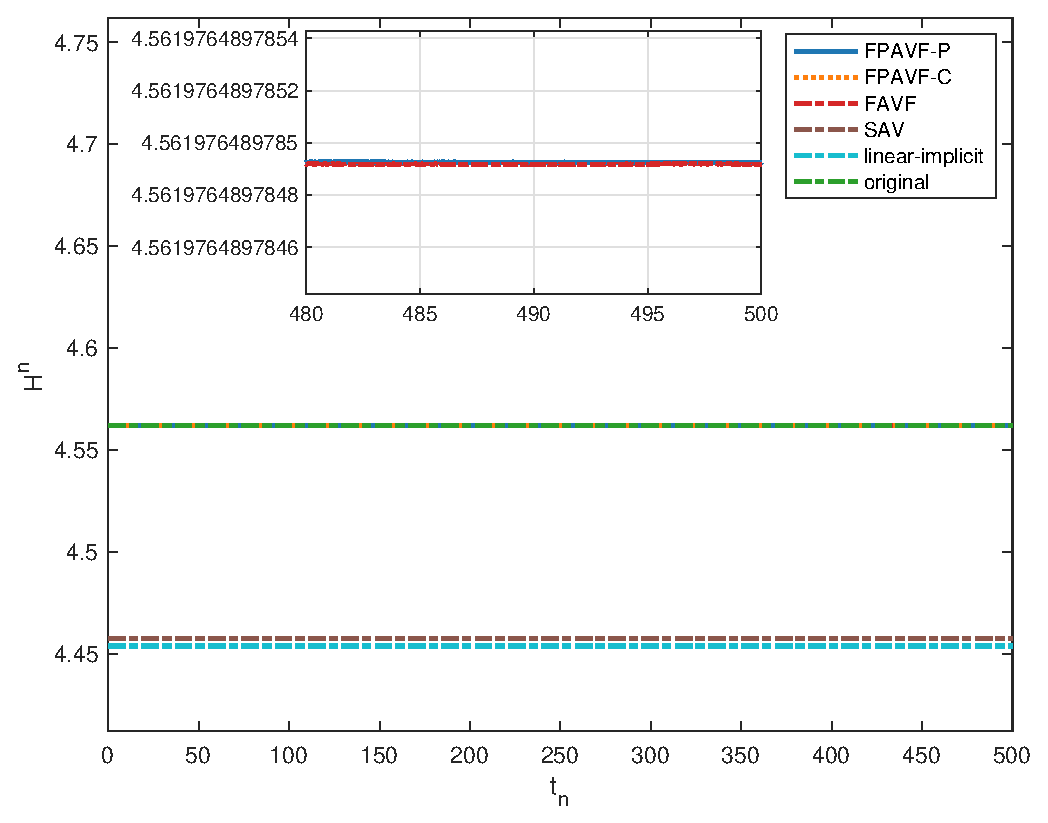
\includegraphics[width=0.5\textwidth]{./figure/exp1_H2.eps}
		%\centerline{($d$) $\alpha=2.0$}
		}
		% \caption{Discrete energy for different $\alpha$ in Example \ref{exp_PAVF:2} with $N = 512$ and $\tau=0.01$.}
		\caption{在例 \ref{exp_PAVF:2} 中,当 $N = 512$ 且 $\tau=0.01$ 时,不同 $\alpha$ 下的离散能量.}
		\label{fig_PAVF:3}
		\end{center}
		\end{figure}
\end{frame}

\begin{frame}%{数值算例}
	\begin{figure}[H]
		\begin{center}
		 \subfigure[$\alpha=1.3$]{ \centering
		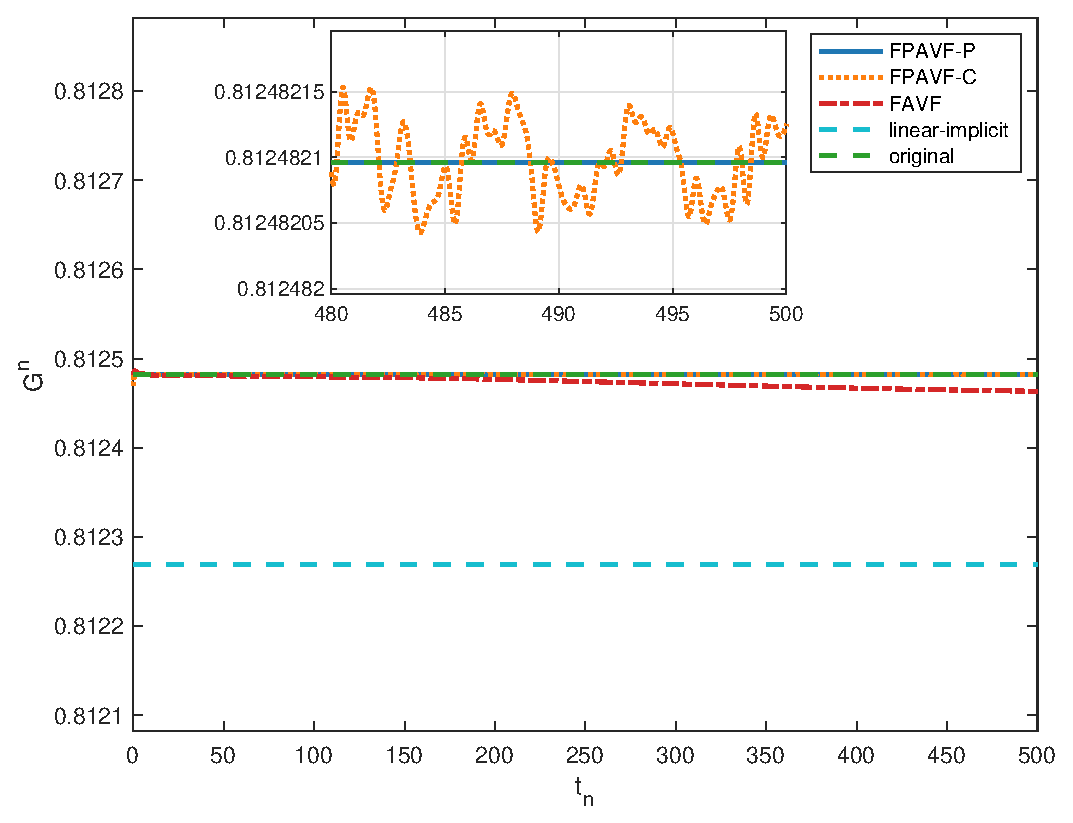
\includegraphics[width=0.5\textwidth]{./figure/exp1_M1.3.eps}
		%\centerline{($a$) $\alpha=1.3$}
		}\subfigure[$\alpha=1.6$]{ \centering
		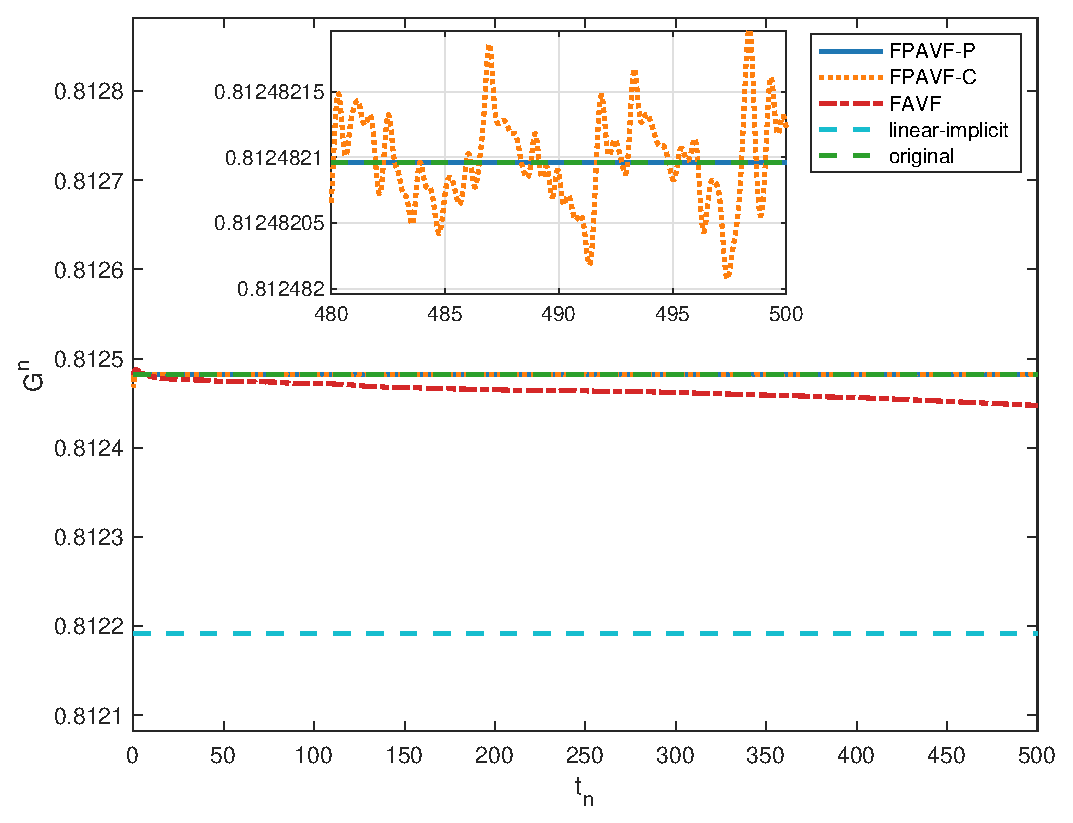
\includegraphics[width=0.5\textwidth]{./figure/exp1_M1.6.eps}
		%\centerline{($b$) $\alpha=1.6$}
		}\caption{在例 \ref{exp_PAVF:2} 中,当 $N = 512$ 且 $\tau=0.01$ 时,不同 $\alpha$ 下的离散质量.}
		 \label{fig_PAVF:4}
		\end{center}
		\end{figure}
\end{frame}

\begin{frame}%{数值算例}
	\begin{figure}[H]
		\begin{center}
		 \subfigure[$\alpha=1.9$]{ \centering
		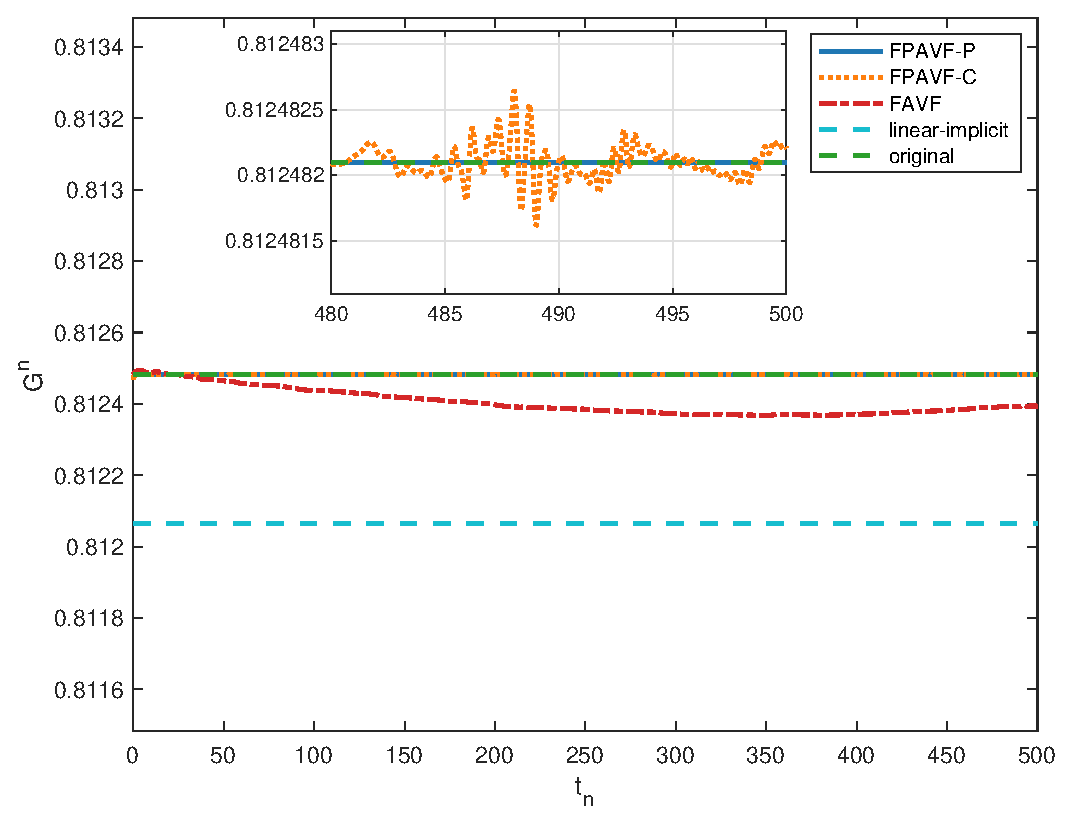
\includegraphics[width=0.5\textwidth]{./figure/exp1_M1.9.eps}
		%\centerline{($c$) $\alpha=1.9$}
		}\subfigure[$\alpha=2.0$]{ \centering
		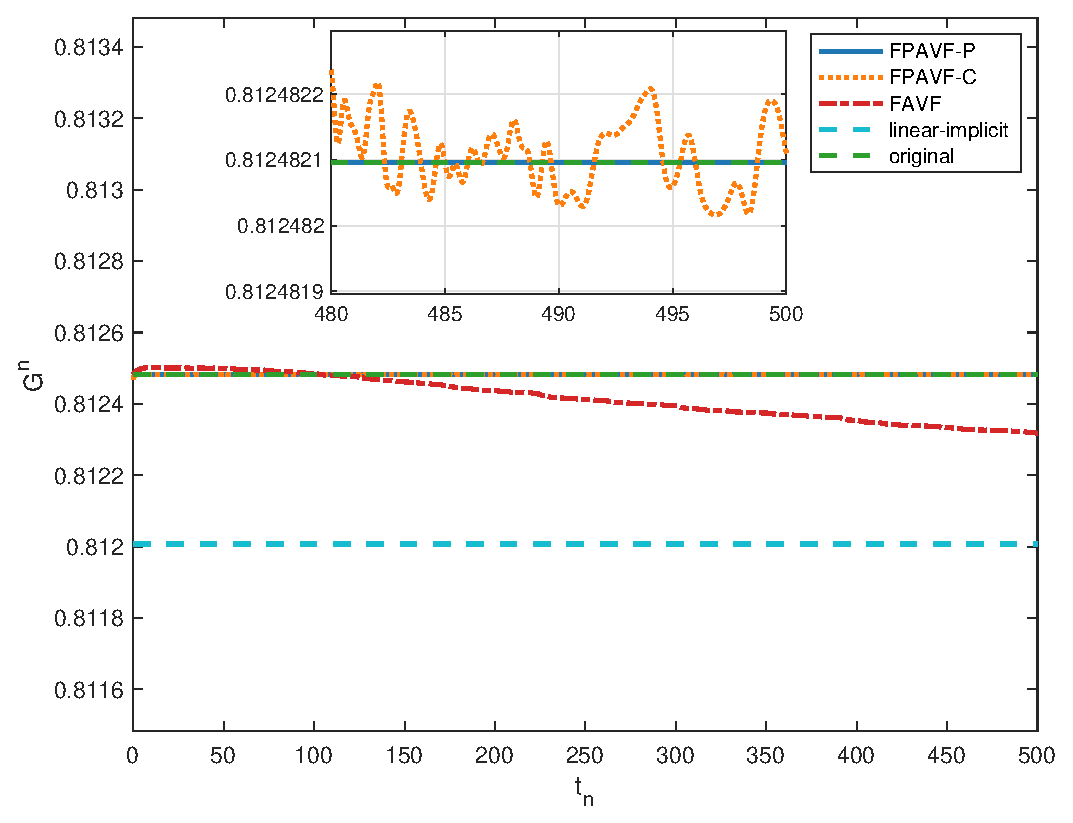
\includegraphics[width=0.5\textwidth]{./figure/exp1_M2.eps}
		%\centerline{($d$) $\alpha=2.0$}
		}
		% \caption{Discrete mass for different $\alpha$ in Example \ref{exp_PAVF:2} with $N = 512$ and $\tau=0.01$.}
		\caption{在例 \ref{exp_PAVF:2} 中,当 $N = 512$ 且 $\tau=0.01$ 时,不同 $\alpha$ 下的离散质量.}
		 \label{fig_PAVF:4}
		\end{center}
		\end{figure}
\end{frame}

\begin{frame}%{数值算例}

	\begin{table}[H]\tiny
		\centering
		% \caption{Discrete energy $H^n$ at time $t=t_n$ for Example \ref{exp_PAVF:2} when $\alpha=2$.}
		\caption{在例 \ref{exp_PAVF:2} 中,当 $\alpha=2.0$ 时,时刻 $t=t_n$ 的离散能量 $H^n$.}
	
		  \begin{tabular}{lllllll}
		  \toprule
		   $t$   &FAVF   &FPAVF   &FPAVF-C   &SAV    &Linear-Implicit   &FPAVF-P\\
		  \midrule
		  0     &4.561976489785   &4.561976489785   &4.561976489785   &4.457414815200   &4.453861069486   &4.561976489785 \\
		  10    &4.561976489785   &4.561976489785   &4.561976489785   &4.457414815200   &4.453861069486   &4.561976489785 \\
		  100   &4.561976489785   &4.561976489785   &4.561976489782   &4.457414815197   &4.453861069489   &4.561976489785 \\
		  200   &4.561976489785   &4.561976489785   &4.561976489779   &4.457414815195   &4.453861069492   &4.561976489785 \\
		  300   &4.561976489785   &4.561976489785   &4.561976489776   &4.457414815192   &4.453861069494   &4.561976489785 \\
		  400   &4.561976489785   &4.561976489785   &4.561976489772   &4.457414815190   &4.453861069497   &4.561976489785 \\
		  500   &4.561976489785   &4.561976489785   &4.561976489768   &4.457414815187   &4.453861069500   &4.561976489785 \\
		  \midrule
		  \multicolumn{7}{r}{Original energy:~4.56197648980619} \\
		  \bottomrule
		  \end{tabular}\label{tab_PAVF:1}%
	  \end{table}%
	
	  \begin{table}[H]\tiny
		\centering
		% \caption{Discrete mass $G^n$ at time $t=t_n$ for Example \ref{exp_PAVF:2} when $\alpha=1.3$.}
		\caption{在例 \ref{exp_PAVF:2} 中,当 $\alpha=1.3$ 时,时刻 $t=t_n$ 的离散质量 $G^n$.}
		  \begin{tabular}{llllll}
		  \toprule
	$t$   &FAVF   &FPAVF   &FPAVF-C   &Linear-Implicit   &FPAVF-P\\
		  \midrule
		  0     &0.812482096011643   &0.812486108372853   &0.812481093228288   &0.812269212105079   &0.812482096009232 \\
		  10    &0.812481652913507   &0.815448411130831   &0.812482228623069   &0.812269212105449   &0.812482096009234 \\
		  100   &0.812479701090339   &0.815337307670638   &0.812482081439882   &0.812269212105119   &0.812482096009236 \\
		  200   &0.812476755660814   &0.815352772611703   &0.812482091028916   &0.812269212105298   &0.812482096009256 \\
		  300   &0.812471706145304   &0.815369448311709   &0.812482102752682   &0.812269212105193   &0.812482096009262 \\
		  400   &0.812466871593141   &0.815375406648485   &0.812482112407629   &0.812269212105361   &0.812482096009263 \\
		  500   &0.812463332390332   &0.815391313914498   &0.812482125179718   &0.812269212105409   &0.812482096009261 \\
		  \midrule
		  \multicolumn{6}{r}{Original mass:~0.812482096009503} \\
		  \bottomrule
		  \end{tabular}\label{tab_PAVF:2}%
	  \end{table}%
\end{frame}

\begin{frame}%{数值算例}

	\begin{table}[H]\tiny
		\centering
		% \caption{Discrete mass $G^n$ at time $t=t_n$ for Example \ref{exp_PAVF:2} when $\alpha=1.6$.}
		\caption{在例 \ref{exp_PAVF:2} 中,当 $\alpha=1.6$ 时,时刻 $t=t_n$ 的离散质量 $G^n$.}
		\begin{tabular}{llllll}
		  \toprule
	$t$   &FAVF   &FPAVF   &FPAVF-C   &Linear-Implicit   &FPAVF-P\\
		  \midrule
		  0     &0.812482096014526   &0.812487932904355   &0.812480637459791   &0.812191342790779   &0.812482096009232 \\
		  10    &0.812479542844467   &0.815290680597744   &0.812482338980161   &0.812191342790869   &0.812482096009234 \\
		  100   &0.812471993678066   &0.814964610988901   &0.812482077830270   &0.812191342790519   &0.812482096009245 \\
		  200   &0.812465076996841   &0.814934135072654   &0.812482168949170   &0.812191342790438   &0.812482096009252 \\
		  300   &0.812461964307183   &0.815026734196011   &0.812482132284732   &0.812191342790211   &0.812482096009255 \\
		  400   &0.812456227758388   &0.815045189971354   &0.812482132454783   &0.812191342790067   &0.812482096009255 \\
		  500   &0.812447472460440   &0.815097180030255   &0.812482122664758   &0.812191342789578   &0.812482096009251 \\
		  \midrule
		  \multicolumn{6}{r}{Original mass:~0.812482096009503} \\
		  \bottomrule
		  \end{tabular}\label{tab_PAVF:3}%
	  \end{table}%

	  \begin{table}[H]\tiny
		\centering
		% \caption{Discrete mass $G^n$ at time $t=t_n$ for Example \ref{exp_PAVF:2} when $\alpha=2$.}
		\caption{在例 \ref{exp_PAVF:2} 中,当 $\alpha=2.0$ 时,时刻 $t=t_n$ 的离散质量 $G^n$.}
		\begin{tabular}{llllll}
		  \toprule
	$t$   &FAVF   &FPAVF   &FPAVF-C   &Linear-Implicit   &FPAVF-P\\
		  \midrule
		  0     &0.812482096027426   &0.812492566135382   &0.812479480708946   &0.812007279829162   &0.812482096009232 \\
		  10    &0.812501574603936   &0.815690689466538   &0.812482208549750   &0.812007279829185   &0.812482096009233 \\
		  100   &0.812485179319911   &0.815559529804266   &0.812482224295188   &0.812007279829068   &0.812482096009234 \\
		  200   &0.812436598720768   &0.815737264057778   &0.812482177481325   &0.812007279828906   &0.812482096009234 \\
		  300   &0.812395565737519   &0.815914179675223   &0.812482122649446   &0.812007279828999   &0.812482096009235 \\
		  400   &0.812353830841431   &0.816227202656059   &0.812482101787071   &0.812007279828969   &0.812482096009235 \\
		  500   &0.812317849493374   &0.816336221770707   &0.812482109657662   &0.812007279829037   &0.812482096009234 \\
		  \midrule
		  \multicolumn{6}{r}{Original mass:~0.812482096009503} \\
		  \bottomrule
		  \end{tabular}\label{tab_PAVF:4}%
	  \end{table}%
\end{frame}

\begin{frame}%{数值算例}

	\begin{figure}[H]
		\begin{center}
		 \subfigure[$\alpha=1.3$]{ \centering
		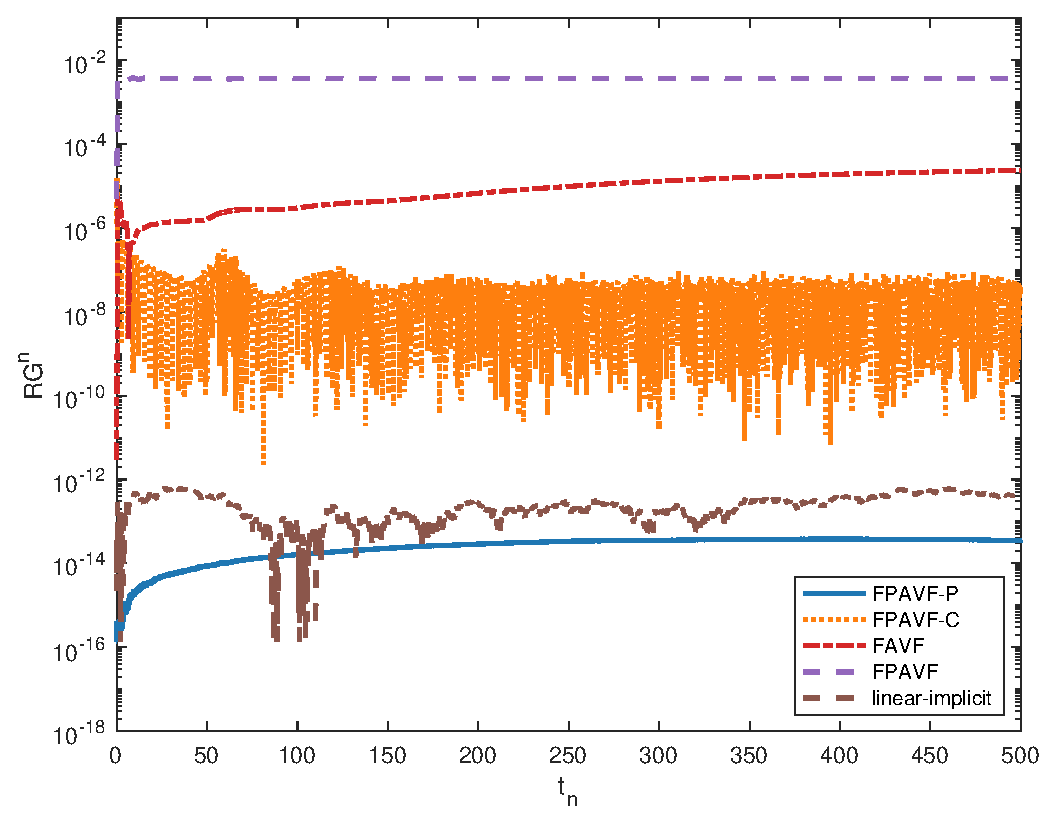
\includegraphics[width=0.3\textwidth]{./figure/exp1_RM1.3.eps}
		%\centerline{($a$) $\alpha=1.3$}
		}\subfigure[$\alpha=1.6$]{ \centering
		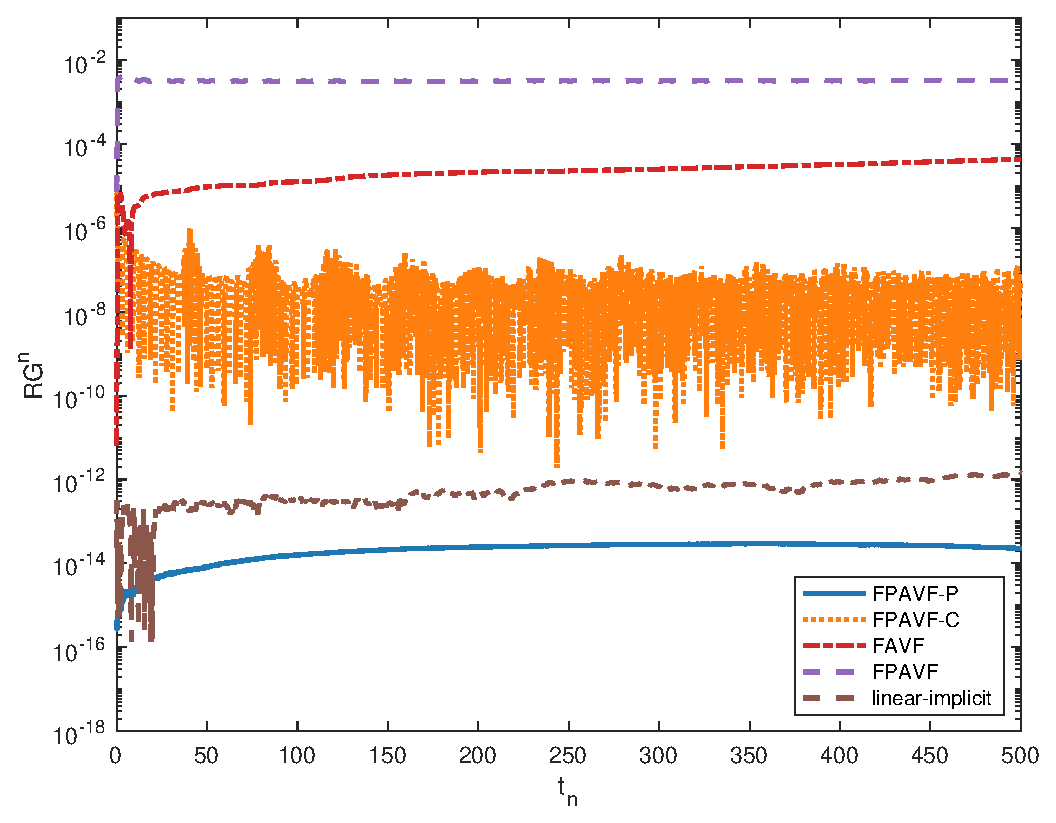
\includegraphics[width=0.3\textwidth]{./figure/exp1_RM1.6.eps}
		%\centerline{($b$) $\alpha=1.6$}
		}\subfigure[$\alpha=1.9$]{ \centering
		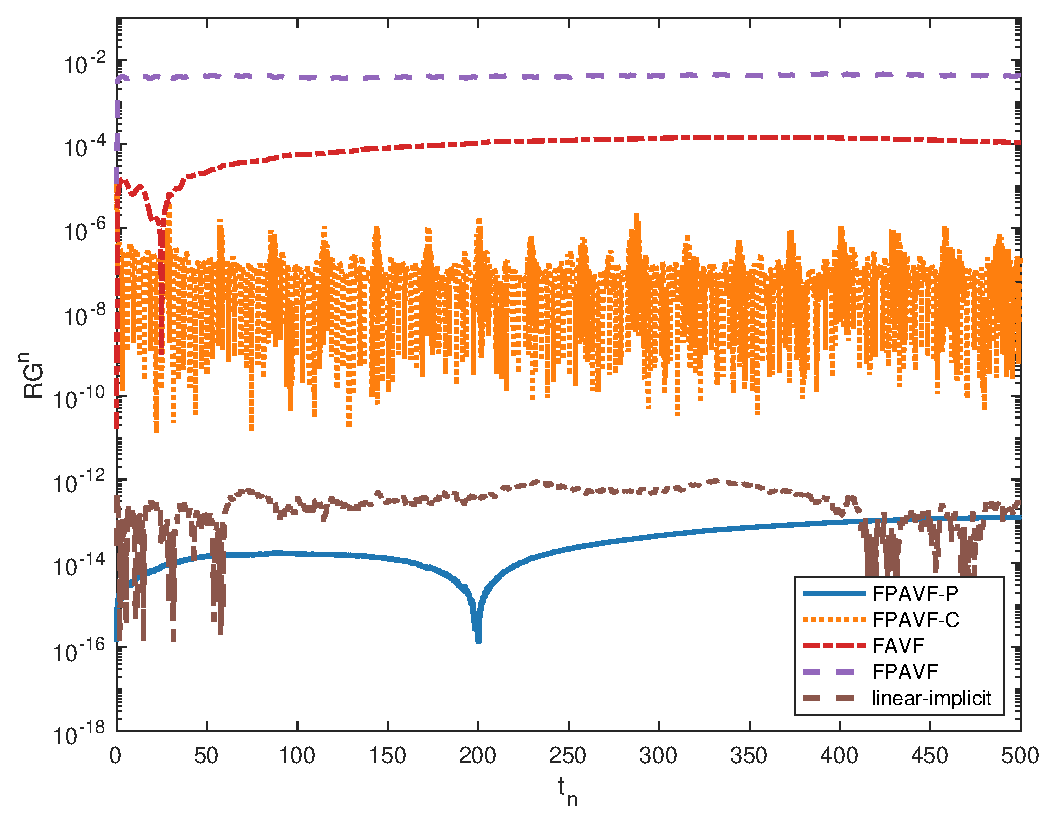
\includegraphics[width=0.3\textwidth]{./figure/exp1_RM1.9.eps}
		%\centerline{($c$) $\alpha=1.9$}
		}
		% \caption{The relative errors of discrete mass for different $\alpha$ in Example \ref{exp_PAVF:2} with $N = 512$ and $\tau=0.01$.}
		\caption{在例 \ref{exp_PAVF:2} 中,当 $N = 512$ 且 $\tau=0.01$ 时,不同 $\alpha$ 下的离散质量相对误差}
		\label{fig_PAVF:5}
		\end{center}
		\end{figure}
\end{frame}

\begin{frame}%{数值算例}
	\begin{figure}[H]
		\begin{center}
		 \subfigure[$\alpha=1.3$]{ \centering
		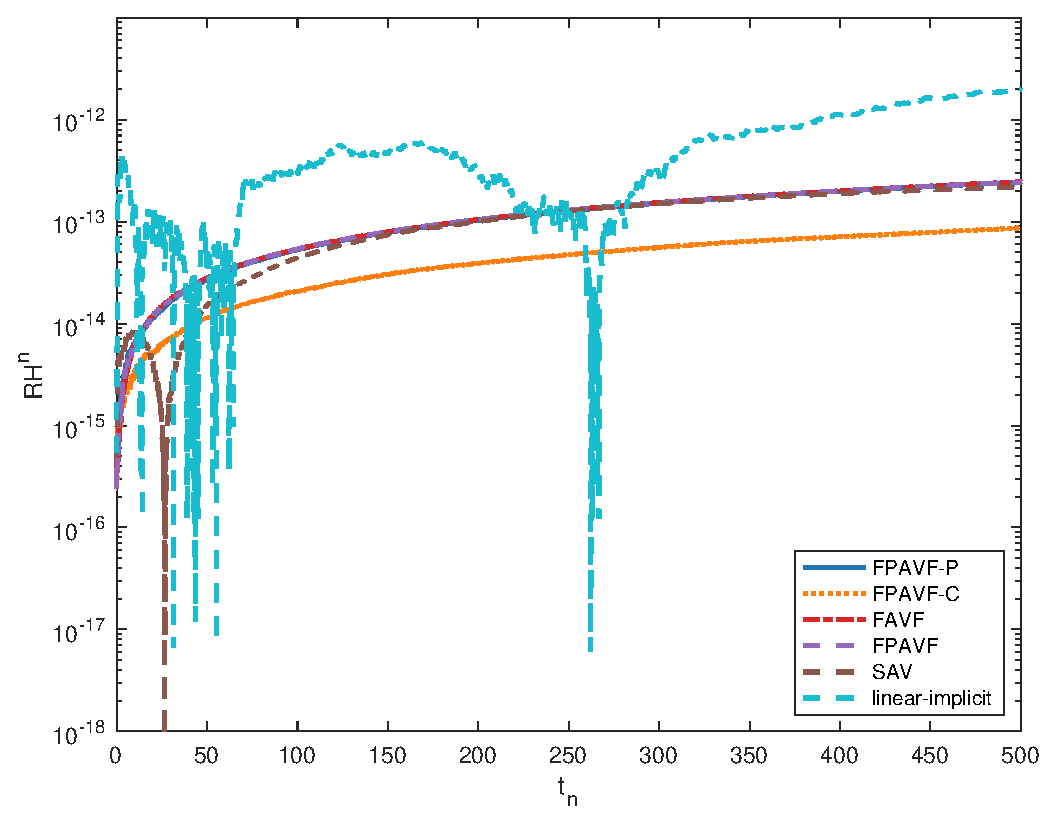
\includegraphics[width=0.3\textwidth]{./figure/exp1_RH1.3.eps}
		%\centerline{($a$) $\alpha=1.3$}
		}\subfigure[$\alpha=1.6$]{ \centering
		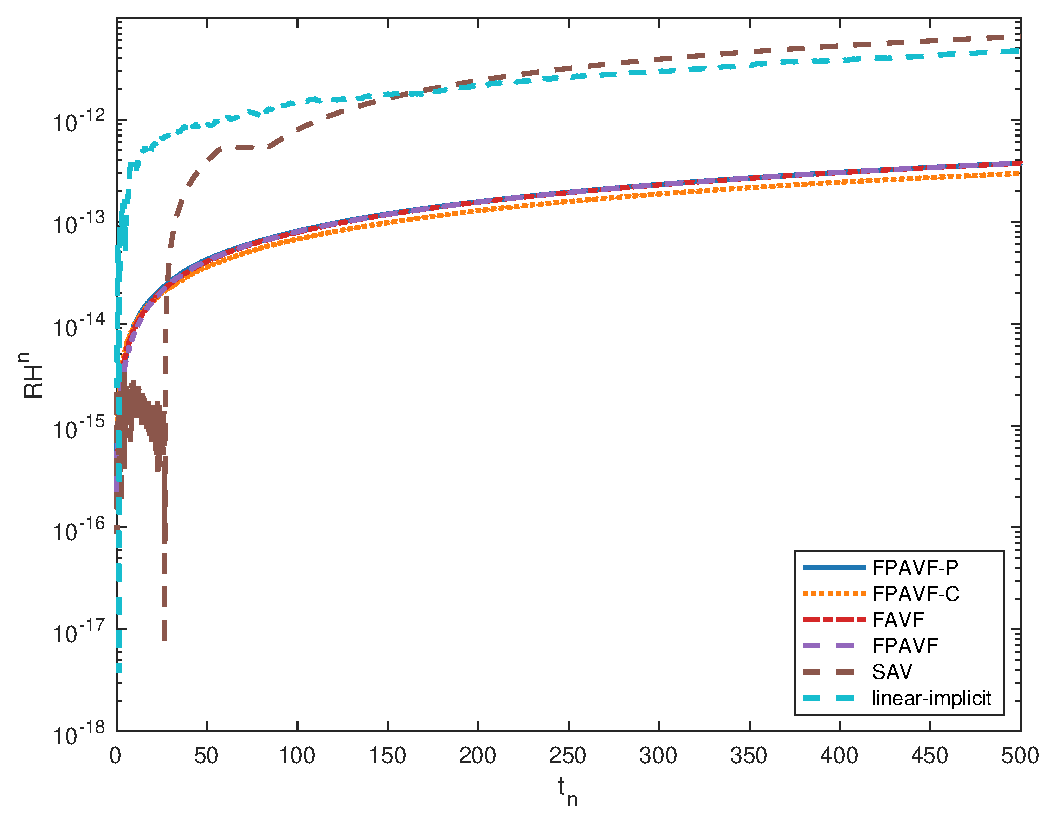
\includegraphics[width=0.3\textwidth]{./figure/exp1_RH1.6.eps}
		%\centerline{($b$) $\alpha=1.6$}
		} \subfigure[$\alpha=1.9$]{ \centering
		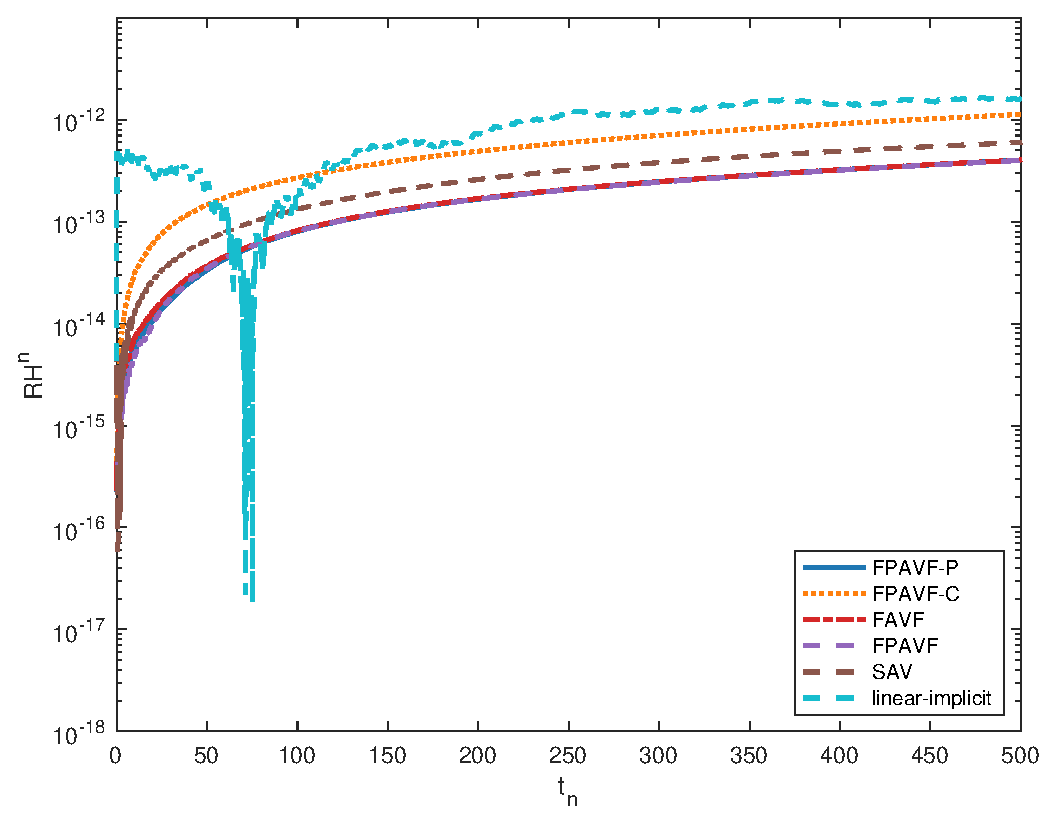
\includegraphics[width=0.3\textwidth]{./figure/exp1_RH1.9.eps}
		%\centerline{($c$) $\alpha=1.9$}
		}
		% \caption{The relative errors of discrete energy for different $\alpha$ in Example \ref{exp_PAVF:2} with $N = 512$ and $\tau=0.01$.} 
		\caption{在例 \ref{exp_PAVF:2} 中,当 $N = 512$ 且 $\tau=0.01$ 时,不同 $\alpha$ 下的离散能量相对误差}\label{fig_PAVF:6}
		\end{center}
		\end{figure}
\end{frame}

\begin{frame}{数值算例}
	\begin{example}\label{exp_PAVF:4}
		考虑带有初始值的二维非线性分数薛定谔波动方程 :
		\begin{equation}\label{eq_PAVF_110}
		u(x,y, 0)=\mbox{sech}\left(x^2+y^2\right), u_t(x,y, 0)=\sin (x+y) \mbox{sech}\left(-2(x^2+y^2)\right), (x,y,t)\in  \Omega\times[0, T],
		\end{equation}
		其中 $\Omega=[-5,5] \times[-5,5]$.
		\end{example}
\end{frame}

\begin{frame}%{数值算例}

	\begin{figure}[H]
		\begin{center}
		\subfigure[$\tau=1/1000$]{ \centering
		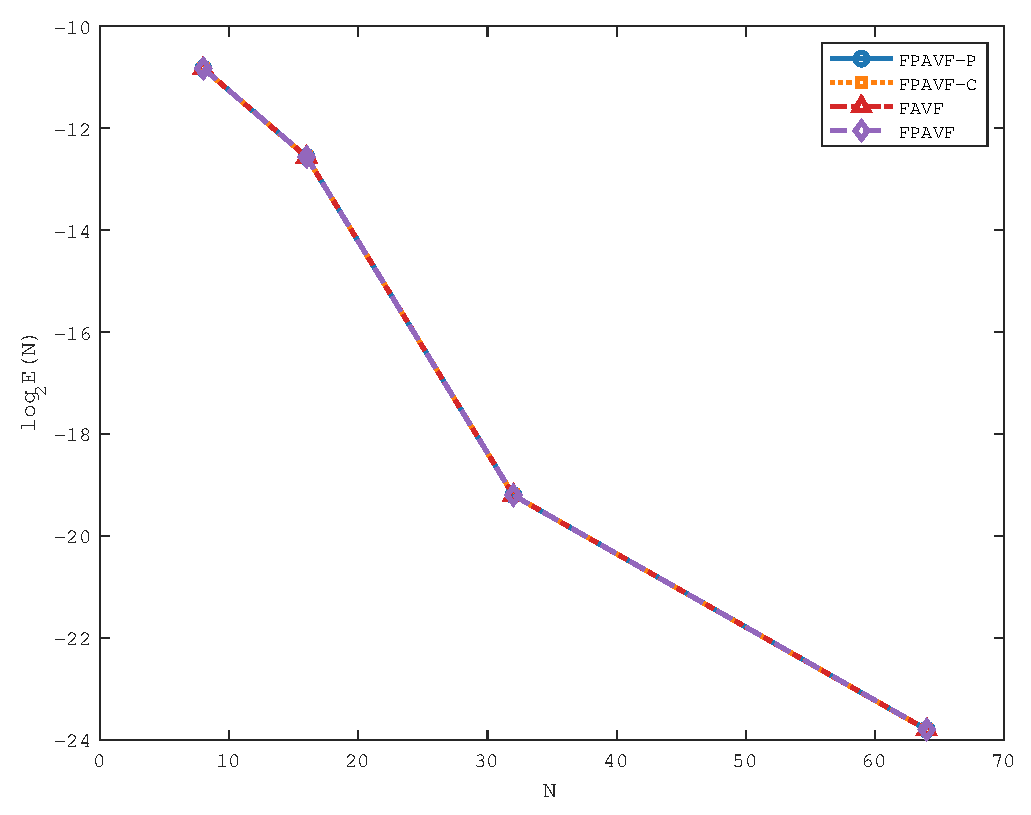
\includegraphics[width=0.5\textwidth]{./figure/exp2_s1.5.eps}
		%\centerline{($b$) Spatial accuracy with $\tau = 10^{-3}.$}
		}\subfigure[$N=16$]{ \centering
		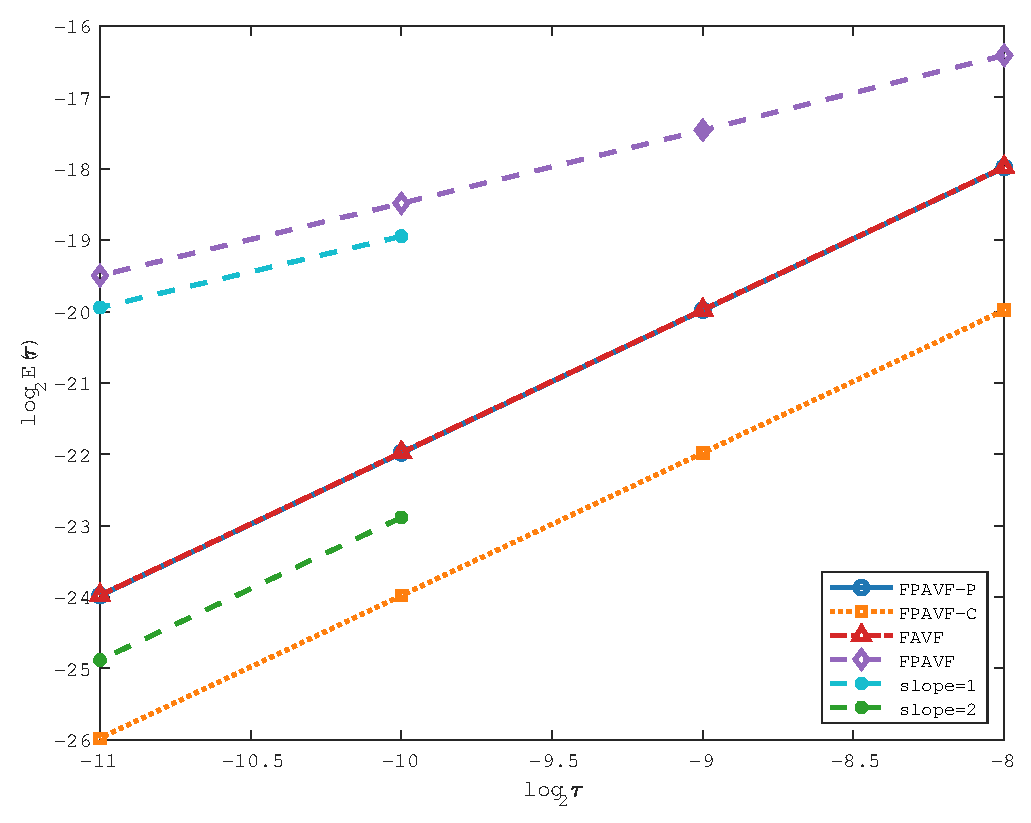
\includegraphics[width=0.5\textwidth]{./figure/exp2_t1.5.eps}
		%\centerline{($a$) Temporal accuracy with $N=128.$}
		}
		% \caption{Convergence orders of four schemes for Example \ref{exp_PAVF:4} with $\alpha=1.5$.} 
		\caption{当$\alpha=1.5$时,例 \ref{exp_PAVF:4} 中四种格式的收敛阶.}
		\label{fig_PAVF:7}
		\end{center}
		\end{figure}
		
\end{frame}

\begin{frame}%{数值算例}
	\begin{figure}[H]
		\begin{center}
		\subfigure[$\tau=1/1000$]{ \centering
		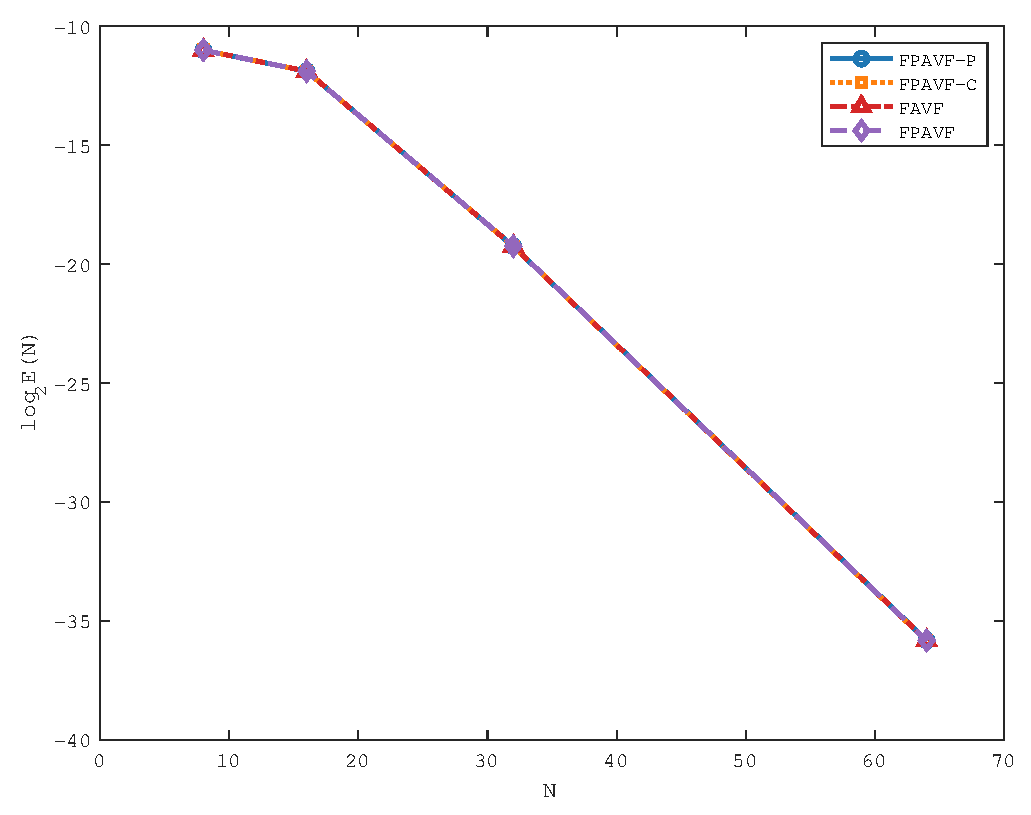
\includegraphics[width=0.5\textwidth]{./figure/exp2_s2.eps}
		%\centerline{($b$) Spatial accuracy with $\tau = 10^{-3}.$}
		}\subfigure[$N=16$]{ \centering
		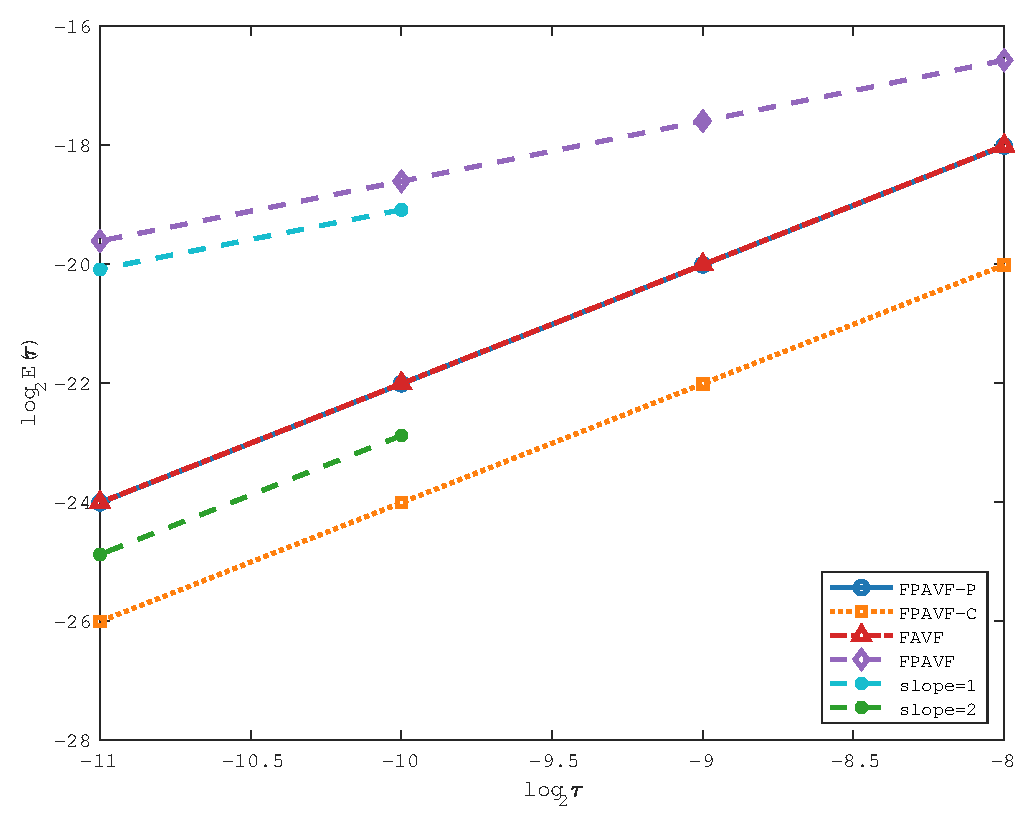
\includegraphics[width=0.5\textwidth]{./figure/exp2_t2.eps}
		%\centerline{($a$) Temporal accuracy with $N=128.$}
		}
		% \caption{Convergence orders of four schemes for Example \ref{exp_PAVF:4} with $\alpha=2.0$.}
		\caption{当$\alpha=2.0$时,例 \ref{exp_PAVF:4} 中四种格式的收敛阶.}
		 \label{fig_PAVF:8}
		\end{center}
		\end{figure}
\end{frame}

\begin{frame}%{数值算例}
	\begin{figure}[H]
		\begin{center}
		 \subfigure[$\alpha=1.3$]{ \centering
		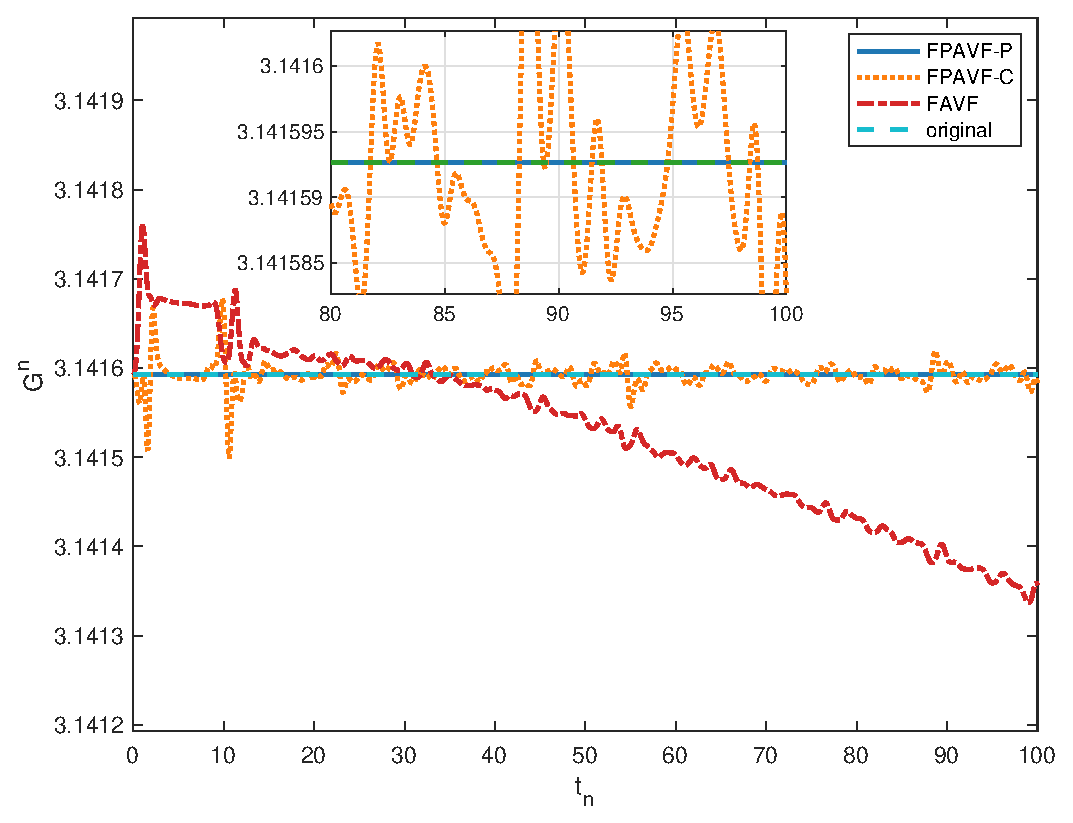
\includegraphics[width=0.5\textwidth]{./figure/exp2_M1.3.eps}
		%\centerline{($a$) $\alpha=1.3$}
		}\subfigure[$\alpha=1.6$]{ \centering
		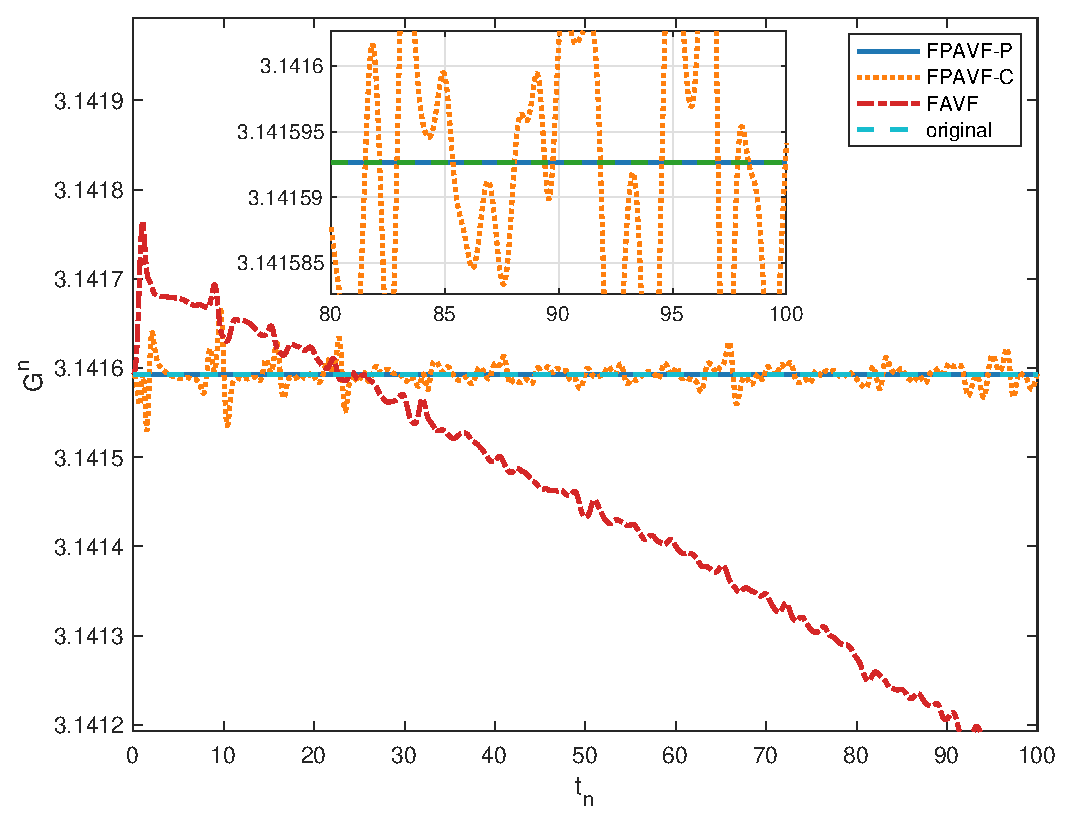
\includegraphics[width=0.5\textwidth]{./figure/exp2_M1.6.eps}
		%\centerline{($b$) $\alpha=1.6$}
		}\caption{在例 \ref{exp_PAVF:4} 中,当 $N = 64$ 且 $\tau=0.01$ 时,不同 $\alpha$ 下的离散质量.}
		\label{fig_PAVF:9}
		\end{center}
		\end{figure}
	
\end{frame}


\begin{frame}%{数值算例}
	\begin{figure}[H]
		\begin{center}
		 \subfigure[$\alpha=1.9$]{ \centering
		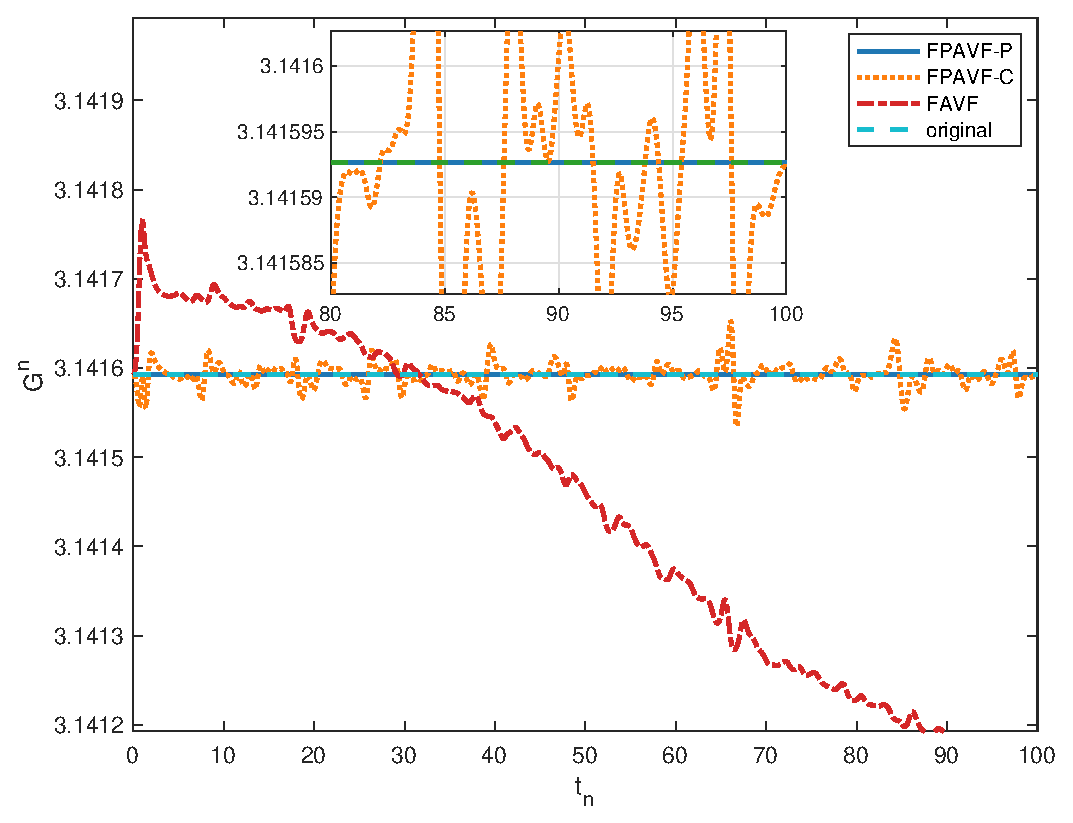
\includegraphics[width=0.5\textwidth]{./figure/exp2_M1.9.eps}
		%\centerline{($c$) $\alpha=1.9$}
		}\subfigure[$\alpha=2.0$]{ \centering
		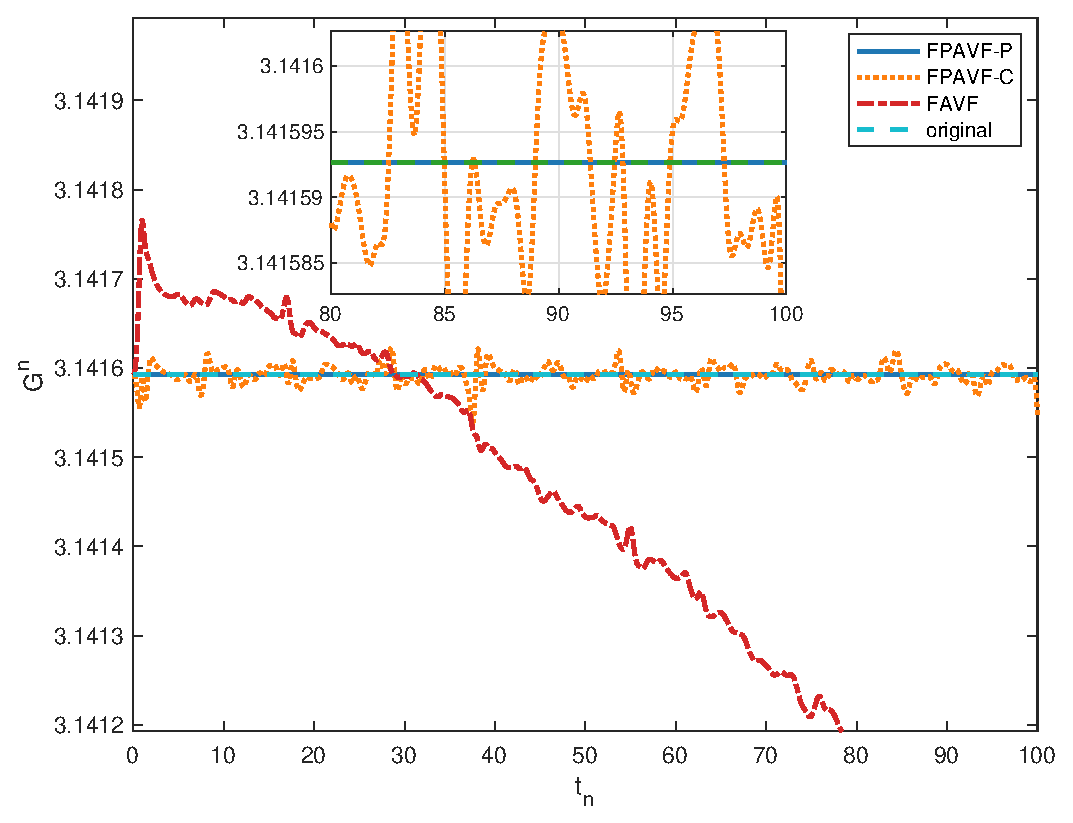
\includegraphics[width=0.5\textwidth]{./figure/exp2_M2.eps}
		%\centerline{($d$) $\alpha=2.0$}
		}
		% \caption{Discrete mass for different $\alpha$ in Example \ref{exp_PAVF:4} with $N = 64$ and $\tau=0.01$.} 
		\caption{在例 \ref{exp_PAVF:4} 中,当 $N = 64$ 且 $\tau=0.01$ 时,不同 $\alpha$ 下的离散质量.}
		\label{fig_PAVF:9}
		\end{center}
		\end{figure}
\end{frame}

\begin{frame}%{数值算例}

	\begin{figure}[H]
		\begin{center}
		\subfigure[$\alpha=1.3$]{ \centering
		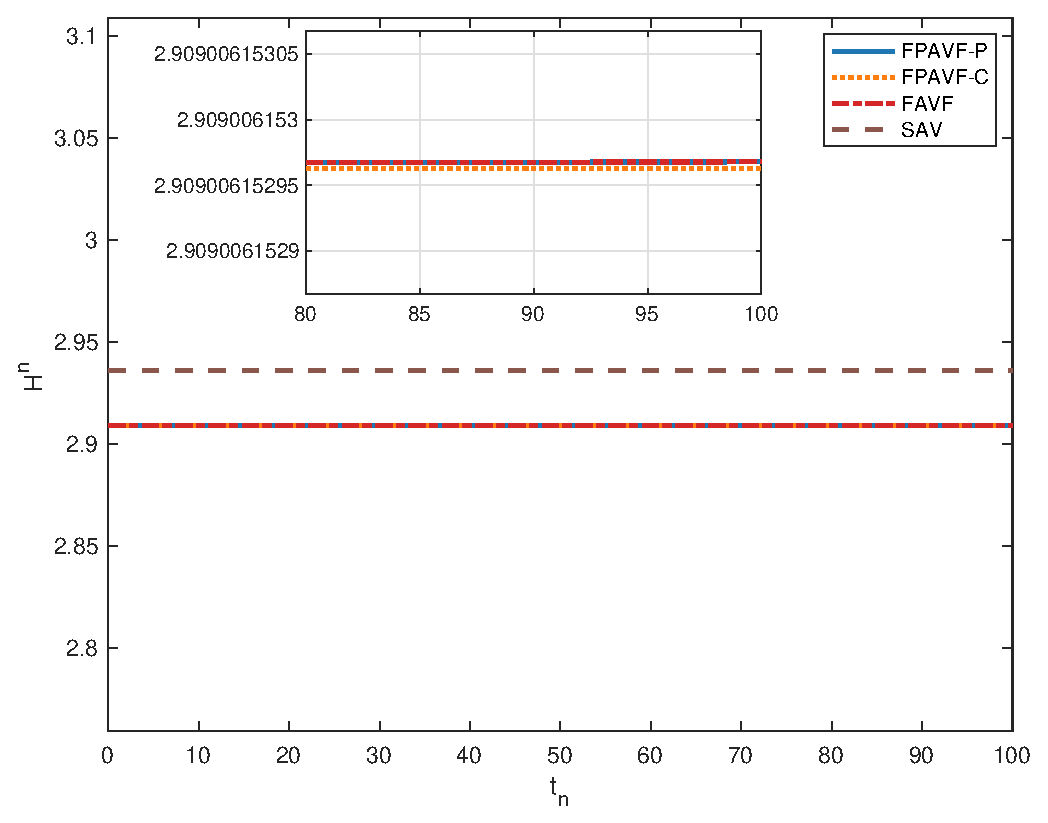
\includegraphics[width=0.5\textwidth]{./figure/exp2_H1.3.eps}
		%\centerline{($a$) $\alpha=1.3$}
		}\subfigure[$\alpha=1.6$]{ \centering
		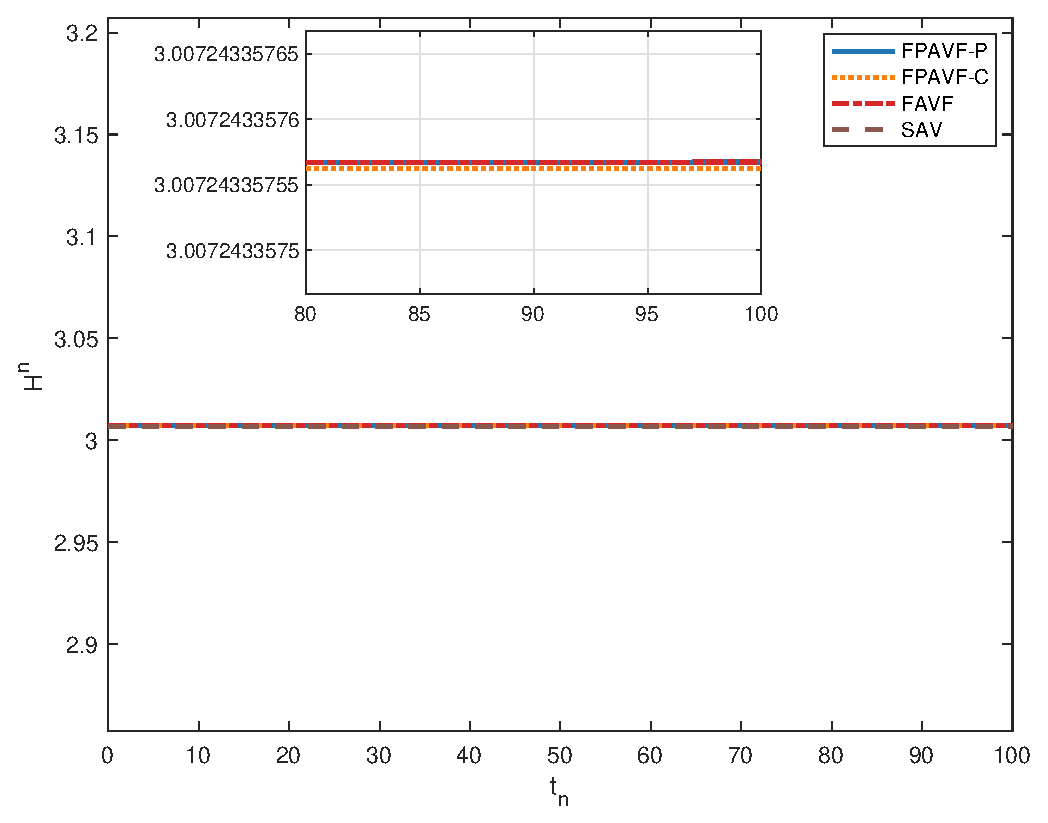
\includegraphics[width=0.5\textwidth]{./figure/exp2_H1.6.eps}
		%\centerline{($b$) $\alpha=1.6$}
		}
		% \caption{Discrete energy for different $\alpha$ in Example \ref{exp_PAVF:4} with $N = 64$ and $\tau=0.01$.} 
		\caption{在例 \ref{exp_PAVF:4} 中,当 $N = 64$ 且 $\tau=0.01$ 时,不同 $\alpha$ 下的离散能量.}
		\label{fig_PAVF:10}
		\end{center}
		\end{figure}
\end{frame}

\begin{frame}%{数值算例}
	\begin{figure}[H]
		\begin{center}
		\subfigure[$\alpha=1.9$]{ \centering
		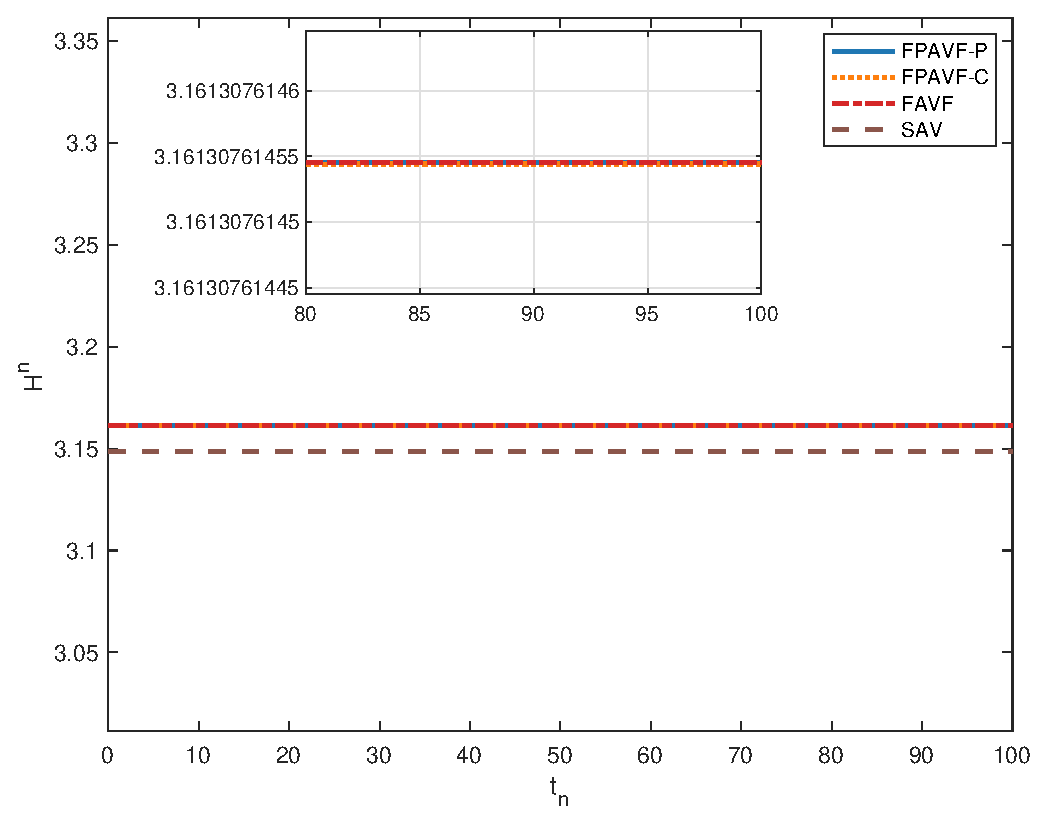
\includegraphics[width=0.5\textwidth]{./figure/exp2_H1.9.eps}
		%\centerline{($d$) $\alpha=2.0$}
		}\subfigure[$\alpha=2.0$]{ \centering
		\includegraphics[width=0.5\textwidth]{./figure/exp2_H2.eps}
		%\centerline{($d$) $\alpha=2.0$}
		}
		% \caption{Discrete energy for different $\alpha$ in Example \ref{exp_PAVF:4} with $N = 64$ and $\tau=0.01$.} 
		\caption{在例 \ref{exp_PAVF:4} 中,当 $N = 64$ 且 $\tau=0.01$ 时,不同 $\alpha$ 下的离散能量.}
		\label{fig_PAVF:10}
		\end{center}
		\end{figure}
\end{frame}

\begin{frame}%{数值算例}
	\begin{figure}[H]
		\begin{center}
		 \subfigure[$\alpha=1.3$]{ \centering
		\includegraphics[width=0.3\textwidth]{./figure/exp2_RM1.3.eps}
		%\centerline{($a$) $\alpha=1.3$}
		}\subfigure[$\alpha=1.6$]{ \centering
		\includegraphics[width=0.3\textwidth]{./figure/exp2_RM1.6.eps}
		%\centerline{($b$) $\alpha=1.6$}
		}\subfigure[$\alpha=1.9$]{ \centering
		\includegraphics[width=0.3\textwidth]{./figure/exp2_RM1.9.eps}
		%\centerline{($c$) $\alpha=1.9$}
		}
		% \caption{The relative errors of discrete mass for different $\alpha$ in Example \ref{exp_PAVF:4} with $N = 64$ and $\tau=0.01$.} 
		\caption{在例 \ref{exp_PAVF:4} 中,当 $N = 64$ 且 $\tau=0.01$ 时,不同 $\alpha$ 下的离散质量相对误差}
		\label{fig_PAVF:11}
		\end{center}
		\end{figure}
\end{frame}

\begin{frame}%{数值算例}
	\begin{figure}[H]
		\begin{center}
		 \subfigure[$\alpha=1.3$]{ \centering
		\includegraphics[width=0.3\textwidth]{./figure/exp2_RH1.3.eps}
		%\centerline{($a$) $\alpha=1.3$}
		}\subfigure[$\alpha=1.6$]{ \centering
		\includegraphics[width=0.3\textwidth]{./figure/exp2_RH1.6.eps}
		%\centerline{($b$) $\alpha=1.6$}
		} \subfigure[$\alpha=1.9$]{ \centering
		\includegraphics[width=0.3\textwidth]{./figure/exp2_RH1.9.eps}
		%\centerline{($c$) $\alpha=1.9$}
		}
		% \caption{The relative errors of discrete energy for different $\alpha$ in Example \ref{exp_PAVF:4} with $N = 64$ and $\tau=0.01$.} 
		\caption{在例 \ref{exp_PAVF:4} 中,当 $N = 64$ 且 $\tau=0.01$ 时,不同 $\alpha$ 下的离散能量相对误差}
		\label{fig_PAVF:12}
		\end{center}
		\end{figure}
\end{frame}

\begin{frame}%{数值算例}
	\begin{table}[H]\tiny
		\centering
		% \caption{Discrete energy $H^n$ at time $t=t_n$ for Example \ref{exp_PAVF:4} when $\alpha=2$.}
		\caption{在例 \ref{exp_PAVF:4} 中,当 $\alpha=2.0$ 时,时刻 $t=t_n$ 的离散能量 $H^n$.}
		\begin{tabular}{llllll}
		  \toprule
		   $t$   &FAVF   &FPAVF   &FPAVF-C   &SAV   &FPAVF-P\\
		  \midrule
		  0     & 3.22697078740176 & 3.22697078740176 & 3.22697078740173 & 3.21234862767094 & 3.22697078740176 \\
		  10    & 3.22697078740176 & 3.22697078740176 & 3.22697078740168 & 3.21234862767062 & 3.22697078740176 \\
		  20    & 3.22697078740176 & 3.22697078740176 & 3.22697078740172 & 3.21234862767066 & 3.22697078740176 \\
		  40    & 3.22697078740175 & 3.22697078740176 & 3.22697078740182 & 3.21234862767033 & 3.22697078740176 \\
		  60    & 3.22697078740176 & 3.22697078740176 & 3.22697078740191 & 3.21234862767035 & 3.22697078740176 \\
		  80    & 3.22697078740176 & 3.22697078740175 & 3.22697078740199 & 3.21234862767073 & 3.22697078740176 \\
		  100   & 3.22697078740175 & 3.22697078740176 & 3.22697078740207 & 3.21234862767045 & 3.22697078740176 \\
		  \midrule
		  \multicolumn{6}{r}{Original energy:~3.22697078976648} \\
		  \bottomrule
		  \end{tabular}\label{tab_PAVF:4-1}%
	  \end{table}%
	
	  % Table generated by Excel2LaTeX from sheet 'Sheet1'
	\begin{table}[H]\tiny
		\centering
		% \caption{Discrete mass $G^n$ at time $t=t_n$ for Example \ref{exp_PAVF:4} when $\alpha=1.3$.}
		\caption{在例 \ref{exp_PAVF:4} 中,当 $\alpha=1.3$ 时,时刻 $t=t_n$ 的离散质量 $G^n$.}
		  \begin{tabular}{lllll}
		  \toprule
	$t$   &FAVF   &FPAVF   &FPAVF-C   &FPAVF-P\\
		  \midrule
		  0     & 3.14159297667455 & 3.14159361842152 & 3.14159241227909 & 3.14159265358976 \\
		  10    & 3.14160952253933 & 3.13595374862870 & 3.14166505643569 & 3.14159265358963 \\
		  20    & 3.14161343543099 & 3.14421089321261 & 3.14158965037808 & 3.14159265358952 \\
		  40    & 3.14157539023564 & 3.14362067013654 & 3.14159917106759 & 3.14159265358932 \\
		  60    & 3.14150249358846 & 3.14217508702013 & 3.14159868539556 & 3.14159265358912 \\
		  80    & 3.14143174175214 & 3.14159826267015 & 3.14158946625201 & 3.14159265358895 \\
		  100   & 3.14135672071641 & 3.14328710863969 & 3.14158227319751 & 3.14159265358880 \\
		  \midrule
		  \multicolumn{5}{r}{Original mass:~3.14159265323701} \\
		  \bottomrule
		  \end{tabular}\label{tab_PAVF:4-2}%
	  \end{table}%
\end{frame}

\begin{frame}%{数值算例}
	\begin{table}[H]\tiny
		\centering
		% \caption{Discrete mass $G^n$ at time $t=t_n$ for Example \ref{exp_PAVF:4} when $\alpha=1.6$.}
		\caption{在例 \ref{exp_PAVF:4} 中,当 $\alpha=1.6$ 时,时刻 $t=t_n$ 的离散质量 $G^n$.}
		 \begin{tabular}{lllll}
		  \toprule
	$t$   &FAVF   &FPAVF   &FPAVF-C   &FPAVF-P\\
		  \midrule
		  0     & 3.14159297668940 & 3.14159361814729 & 3.14159241218683 & 3.14159265358976 \\
		  10    & 3.14163389358031 & 3.13754191888209 & 3.14160072631792 & 3.14159265358928 \\
		  20    & 3.14161716177523 & 3.14433222488425 & 3.14159044899067 & 3.14159265358919 \\
		  40    & 3.14149554093894 & 3.14475213344308 & 3.14160500647197 & 3.14159265358901 \\
		  60    & 3.14139997924855 & 3.14288256207779 & 3.14160023436812 & 3.14159265358885 \\
		  80    & 3.14127488637752 & 3.14241392600216 & 3.14158768432513 & 3.14159265358871 \\
		  100   & 3.14115287766347 & 3.14489331385338 & 3.14159412822417 & 3.14159265358860 \\
			\midrule
		  \multicolumn{5}{r}{Original mass:~3.14159265323701} \\
		  \bottomrule
		  \end{tabular}\label{tab_PAVF:4-3}%
	  \end{table}%
	
	  % Table generated by Excel2LaTeX from sheet 'Sheet1'
	\begin{table}[H]\tiny
		\centering
		% \caption{Discrete mass $G^n$ at time $t=t_n$ for Example \ref{exp_PAVF:4} when $\alpha=2$.}
		\caption{在例 \ref{exp_PAVF:4} 中,当 $\alpha=2.0$ 时,时刻 $t=t_n$ 的离散质量 $G^n$.}
		\begin{tabular}{lllll}
		  \toprule
	$t$   &FAVF   &FPAVF   &FPAVF-C   &FPAVF-P\\
		  \midrule
		  0     & 3.14159297725470 & 3.14159361919902 & 3.14159241149324 & 3.14159265358976 \\
		  10    & 3.14168000260412 & 3.14369215006721 & 3.14160070161208 & 3.14159265358976 \\
		  20    & 3.14164544531849 & 3.14521250122401 & 3.14158745249453 & 3.14159265358976 \\
		  40    & 3.14150535695500 & 3.14531702832209 & 3.14160031804829 & 3.14159265358976 \\
		  60    & 3.14136438511727 & 3.14552013864766 & 3.14159560564481 & 3.14159265358976 \\
		  80    & 3.14118013227991 & 3.14739329967543 & 3.14158800109644 & 3.14159265358976 \\
		  100   & 3.14101125059928 & 3.15011874273391 & 3.14154787019595 & 3.14159265358976 \\
		  \midrule
		  \multicolumn{5}{r}{Original mass:~3.14159265323701} \\
		  \bottomrule
		  \end{tabular}\label{tab_PAVF:4-4}%
	  \end{table}%
\end{frame}

\begin{frame}%{数值算例}
	\begin{figure}[H]
		\begin{center}
		 \subfigure[$\alpha=1.3$]{ \centering
		\includegraphics[width=0.3\textwidth]{./figure/exp2_contour3_p0.eps}
		}\subfigure[$\alpha=1.99$]{ \centering
		\includegraphics[width=0.3\textwidth]{./figure/exp2_contour99_p0.eps}
		} \subfigure[$\alpha=2$]{ \centering
		\includegraphics[width=0.3\textwidth]{./figure/exp2_contour2_p0.eps}
		}
		\caption{示例 \ref{exp_PAVF:4} 中,不同 $\alpha$ 在 $t=0s$ 的波传播图.}
		% \caption{The pictures of wave propagation for Example \ref{exp_PAVF:4} with $\alpha=1.3.$}
		\label{fig_PAVF:13}
		\end{center}
		\end{figure}
\end{frame}

\begin{frame}%{数值算例}
	\begin{figure}[H]
		\begin{center}
		 \subfigure[$\alpha=1.3$]{ \centering
		\includegraphics[width=0.3\textwidth]{./figure/exp2_contour3_p1.eps}
		}\subfigure[$\alpha=1.99$]{ \centering
		\includegraphics[width=0.3\textwidth]{./figure/exp2_contour99_p1.eps}
		} \subfigure[$\alpha=2$]{ \centering
		\includegraphics[width=0.3\textwidth]{./figure/exp2_contour2_p1.eps}
		}
		\caption{示例 \ref{exp_PAVF:4} 中,不同 $\alpha$ 在 $t=1s$ 的波传播图.}
		% \caption{The pictures of wave propagation for Example \ref{exp_PAVF:4} with $\alpha=1.3.$}
		\label{fig_PAVF:13}
		\end{center}
		\end{figure}
\end{frame}

\begin{frame}%{数值算例}
	\begin{figure}[H]
		\begin{center}
		 \subfigure[$\alpha=1.3$]{ \centering
		\includegraphics[width=0.3\textwidth]{./figure/exp2_contour3_p5.eps}
		}\subfigure[$\alpha=1.99$]{ \centering
		\includegraphics[width=0.3\textwidth]{./figure/exp2_contour99_p5.eps}
		} \subfigure[$\alpha=2$]{ \centering
		\includegraphics[width=0.3\textwidth]{./figure/exp2_contour2_p5.eps}
		}
		\caption{示例 \ref{exp_PAVF:4} 中,不同 $\alpha$ 在 $t=5s$ 的波传播图.}
		% \caption{The pictures of wave propagation for Example \ref{exp_PAVF:4} with $\alpha=1.3.$}
		\label{fig_PAVF:13}
		\end{center}
		\end{figure}
\end{frame}

\begin{frame}%{数值算例}
	\begin{figure}[H]
		\begin{center}
		 \subfigure[$\alpha=1.3$]{ \centering
		\includegraphics[width=0.3\textwidth]{./figure/exp2_contour3_p10.eps}
		}\subfigure[$\alpha=1.99$]{ \centering
		\includegraphics[width=0.3\textwidth]{./figure/exp2_contour99_p10.eps}
		} \subfigure[$\alpha=2$]{ \centering
		\includegraphics[width=0.3\textwidth]{./figure/exp2_contour2_p10.eps}
		}
		\caption{示例 \ref{exp_PAVF:4} 中,不同 $\alpha$ 在 $t=10s$ 的波传播图.}
		% \caption{The pictures of wave propagation for Example \ref{exp_PAVF:4} with $\alpha=1.3.$}
		\label{fig_PAVF:13}
		\end{center}
		\end{figure}
\end{frame}

\begin{frame}%{数值算例}
	\begin{figure}[H]
		\begin{center}
		 \subfigure[$\alpha=1.3$]{ \centering
		\includegraphics[width=0.3\textwidth]{./figure/exp2_contour3_p50.eps}
		}\subfigure[$\alpha=1.99$]{ \centering
		\includegraphics[width=0.3\textwidth]{./figure/exp2_contour99_p50.eps}
		} \subfigure[$\alpha=2$]{ \centering
		\includegraphics[width=0.3\textwidth]{./figure/exp2_contour2_p50.eps}
		}
		\caption{示例 \ref{exp_PAVF:4} 中,不同 $\alpha$ 在 $t=50s$ 的波传播图.}
		% \caption{The pictures of wave propagation for Example \ref{exp_PAVF:4} with $\alpha=1.3.$}
		\label{fig_PAVF:13}
		\end{center}
		\end{figure}
\end{frame}

\begin{frame}%{数值算例}
	\begin{figure}[H]
		\begin{center}
		 \subfigure[$\alpha=1.3$]{ \centering
		\includegraphics[width=0.3\textwidth]{./figure/exp2_contour3_p100.eps}
		}\subfigure[$\alpha=1.99$]{ \centering
		\includegraphics[width=0.3\textwidth]{./figure/exp2_contour99_p100.eps}
		} \subfigure[$\alpha=2$]{ \centering
		\includegraphics[width=0.3\textwidth]{./figure/exp2_contour2_p100.eps}
		}
		\caption{示例 \ref{exp_PAVF:4} 中,不同 $\alpha$ 在 $t=100s$ 的波传播图.}
		% \caption{The pictures of wave propagation for Example \ref{exp_PAVF:4} with $\alpha=1.3.$}
		\label{fig_PAVF:13}
		\end{center}
		\end{figure}
\end{frame}

\begin{frame}{小结}
	在本章中,首先重构 NFSWEs 为一个等效的哈密顿系统.
通过将分区平均向量场加方法与傅里叶拟谱方法结合,基于得到的哈密顿系统构建了一个保结构格式.
理论分析和数值结果表明,所提出的方法能够有效地\textcolor[rgb]{0.227,0.373,0.306}{保持原始能量和原始质量守恒.}
\end{frame}

\section{总结展望}
\begin{frame}{总结展望}
	\begin{block}{主要工作}
			\begin{itemize}
				\item \textcolor[rgb]{0.227,0.373,0.306}{SAV-RRK:} 通过SAV方法将NFSWEs的非二次能量转化为新变量的二次形式,结合显式RK方法和松弛技术,提出了一种任意高阶的显式保结构数值格式.
				\item \textcolor[rgb]{0.227,0.373,0.306}{FPAVF-P:} 成功推导了具有周期边界条件的二维NFSWEs的\textcolor[rgb]{0.227,0.373,0.306}{哈密顿形式},引入了分区平均向量场(PAVF)方法,并采用PAVF-P方法构建了能够同时守恒原始能量和质量的数值格式.
				\item \textcolor[rgb]{0.227,0.373,0.306}{谱方法:} 本文使用了傅里叶拟谱方法,作为空间离散方法,充分利用了其非局部性质和傅里叶基函数的特性,通过快速傅里叶变换(FFT)提高了计算效率.
			\end{itemize}
			% 综合而言,本文在NFSWEs数值求解方面取得了新的研究成果,提出的方法在长时间仿真具有良好的适用性,为未来相关研究提供了有益的参考.
		\end{block}
		
\end{frame}

\begin{frame}{总结展望}
	\begin{block}{主要工作}
	本课题为二维NFSWEs构建:
	\begin{itemize}
		\item 任意高阶显式保结构数值格式.
		\item 能够同时保持原始能量和原始质量守恒的数值格式.
	\end{itemize}
\begin{table}[htbp]
	\centering
	% \caption{本课题的目标是为二维NFSWEs构建高效的显式保结构格式以及能够同时保持原始能量和质量的格式}
	  \begin{tabular}{cccccc}
	  \toprule
	  \textcolor[rgb]{0.227,0.373,0.306}{} & \textcolor[rgb]{0.227,0.373,0.306}{\textbf{维度}} & \textcolor[rgb]{0.227,0.373,0.306}{\textbf{空间精度}} & \textcolor[rgb]{0.227,0.373,0.306}{\textbf{时间精度}} & \textcolor[rgb]{0.227,0.373,0.306}{\textbf{能量守恒}} & \textcolor[rgb]{0.227,0.373,0.306}{\textbf{质量守恒}} \\
	  \midrule
	  \textcolor[rgb]{0.227,0.373,0.306}{\textbf{SAV-RRK}} & \textcolor{purple}{2 维}   & \textcolor{purple}{谱精度}   & \textcolor{purple}{任意高阶}  & 修正能量  & 无 \\
	  \midrule
	  \textcolor[rgb]{0.227,0.373,0.306}{\textbf{FPAVF-P}} & \textcolor{purple}{2 维}   & \textcolor{purple}{谱精度}   & 2 阶   & \textcolor{purple}{原始能量}  & \textcolor{purple}{原始质量} \\
	  \bottomrule
	  \end{tabular}%
	\label{tab:3}%
  \end{table}%
\end{block}
\end{frame}

\begin{frame}{总结展望}
	\begin{block}{研究展望}
		% {\footnotesize }
		在本文的基础上及研究过程中, 发现存在以下改进空间:
		\begin{enumerate}
			\item \textcolor[rgb]{0.227,0.373,0.306}{推广到高维问题:}目前研究主要集中在二维问题的差分格式上,未来可将这些方法推广至更高维度,以数值求解三维或更高维度的分数阶方程.
			\item \textcolor[rgb]{0.227,0.373,0.306}{深入分析稳定性和收敛性:}本文尚未对数值方法的收敛性及稳定性进行充分的分析.未来考虑对提出的数值方法进行更深入的稳定性和收敛性分析,以验证其可靠性和有效性.
			\item \textcolor[rgb]{0.227,0.373,0.306}{提高PAVF-P方法的收敛阶:}本文仅构建了PAVF-P的二阶的数值格式,未来的研究可以考虑构建更高阶的数值格式,以进一步提高数值方法的精度.
		\end{enumerate}
	\end{block}
\end{frame}
	
\section{参考文献}

\begin{frame}[allowframebreaks]
	% \tiny
	\scriptsize
	% \footnotesize
\bibliographystyle{acm} 
\bibliography{/Users/turingscat/Zotero/better-bibtex/mylibrary.bib}
% \begin{thebibliography}{77}
%     \providecommand{\natexlab}[1]{#1}
%     \providecommand{\url}[1]{#1}
%     \expandafter\ifx\csname urlstyle\endcsname\relax\else
%       \urlstyle{same}\fi
%     \expandafter\ifx\csname href\endcsname\relax
%       \DeclareUrlCommand\doi{\urlstyle{rm}}
%       \def\eprint#1#2{#2}
%     \else
%       \def\doi#1{\href{https://doi.org/#1}{\nolinkurl{#1}}}
%       \let\eprint\href
%     \fi
    
%     \bibitem[Samko et~al.(1993)Samko, Kilbas, and Marichev]{samkoFractionalIntegralsDerivatives1993}
%     Samko S~G, Kilbas A~A, Marichev O~I.
%     \newblock Fractional integrals and derivatives: Vol.~1\allowbreak[M].
%     \newblock {Gordon and breach science publishers, Yverdon Yverdon-les-Bains, Switzerland}, 1993.
    
%     \bibitem[liI(2015)]{liIntroductionFractionalCalculus2015}
%     \href{https://www.taylorfrancis.com/books/9781482253818/chapters/10.1201/b18503-6}{Introduction to {{Fractional Calculus}}}\allowbreak[M].
%     \newblock 0th ed.
%     \newblock {Chapman and Hall/CRC}, 2015: 19-46.
    
%     \bibitem[Han(2008)]{HandbookDifferentialEquations2008}
%     \href{https://linkinghub.elsevier.com/retrieve/pii/S1874573308X80167}{Handbook of {{Differential Equations}}: {{Stationary Partial Differential Equations}}: Vol.~6\ handbook of {{Differential Equations}} - {{Stationary Partial Differential Equations}}}\allowbreak[M].
%     \newblock {Elsevier}, 2008.
    
%     \bibitem[bry(2008)]{brychkovIndefiniteIntegrals2008}
%     \href{https://www.taylorfrancis.com/books/9781584889571/chapters/10.1201/9781584889571-7}{Indefinite {{Integrals}}}\allowbreak[M].
%     \newblock 0th ed.
%     \newblock {Chapman and Hall/CRC}, 2008: 121-130.
    
%     \bibitem[Zhang et~al.(2005)Zhang, Crawford, Deeks, Stutter, Bengough, and Young]{zhangMassBalanceBased2005}
%     Zhang X, Crawford J~W, Deeks L~K, et~al.
%     \newblock \href{http://doi.wiley.com/10.1029/2004WR003818}{A mass balance based numerical method for the fractional advection-dispersion equation: {{Theory}} and application: {{FRACTIONAL ADVECTION-DISPERSION EQUATION}}}\allowbreak[J].
%     \newblock Water Resour Res, 2005, 41\allowbreak (7).
    
%     \bibitem[Carreras et~al.(2001)Carreras, Lynch, and Zaslavsky]{carrerasAnomalousDiffusionExit2001}
%     Carreras B~A, Lynch V~E, Zaslavsky G~M.
%     \newblock \href{http://aip.scitation.org/doi/10.1063/1.1416180}{Anomalous diffusion and exit time distribution of particle tracers in plasma turbulence model}\allowbreak[J].
%     \newblock Phys Plasmas, 2001, 8\allowbreak (12): 5096-5103.
    
%     \bibitem[Hilfer(2000)]{hilferFRACTIONALCALCULUSREGULAR2000}
%     Hilfer R.
%     \newblock \href{http://www.worldscientific.com/doi/abs/10.1142/9789812817747_0009}{{{FRACTIONAL CALCULUS AND REGULAR VARIATION IN THERMODYNAMICS}}}\allowbreak[M].
%     \newblock {WORLD SCIENTIFIC}, 2000: 429-463.
    
%     \bibitem[Magin et~al.(2009)Magin, Feng, and Baleanu]{maginSolvingFractionalOrder2009}
%     Magin R, Feng X, Baleanu D.
%     \newblock \href{https://onlinelibrary.wiley.com/doi/10.1002/cmr.a.20129}{Solving the fractional order {{Bloch}} equation}\allowbreak[J].
%     \newblock Concept Magn Reson A, 2009, 34A\allowbreak (1): 16-23.
    
%     \bibitem[Zaslavsky et~al.(1993)Zaslavsky, Stevens, and Weitzner]{zaslavskySelfsimilarTransportIncomplete1993}
%     Zaslavsky G~M, Stevens D, Weitzner H.
%     \newblock \href{https://link.aps.org/doi/10.1103/PhysRevE.48.1683}{Self-similar transport in incomplete chaos}\allowbreak[J].
%     \newblock Phys Rev E, 1993, 48\allowbreak (3): 1683-1694.
    
%     \bibitem[Sun et~al.(2011)Sun, Chen, and Chen]{sunRandomorderFractionalDifferential2011}
%     Sun H, Chen Y, Chen W.
%     \newblock \href{https://linkinghub.elsevier.com/retrieve/pii/S0165168410000447}{Random-order fractional differential equation models}\allowbreak[J].
%     \newblock Signal Process, 2011, 91\allowbreak (3): 525-530.
    
%     \bibitem[Tsutsumi(1984)]{tsutsumiNonrelativisticApproximationNonlinear1984}
%     Tsutsumi M.
%     \newblock \href{https://www.sciencedirect.com/science/article/pii/0362546X84900087}{Nonrelativistic approximation of nonlinear {{Klein-Gordon}} equations in two space dimensions}\allowbreak[J].
%     \newblock Nonlinear Analysis: Theory, Methods \& Applications, 1984, 8\allowbreak (6): 637-643.
    
%     \bibitem[Machihara et~al.(2002)Machihara, Nakanishi, and Ozawa]{machiharaNonrelativisticLimitEnergy2002}
%     Machihara S, Nakanishi K, Ozawa T.
%     \newblock \href{http://link.springer.com/10.1007/s002080200008}{Nonrelativistic limit in the energy space for nonlinear {{Klein-Gordon}} equations}\allowbreak[J].
%     \newblock Math Ann, 2002, 322\allowbreak (3): 603-621.
    
%     \bibitem[Colin et~al.(Tue Jun 30 20:00:00 EDT 1998)Colin and Fabrie]{colinSemidiscretizationTimeNonlinear1998}
%     Colin T, Fabrie P.
%     \newblock \href{https://www.aimsciences.org/en/article/doi/10.3934/dcds.1998.4.671}{Semidiscretization in time for nonlinear {{Schr{\"o}dinger-waves}} equations}\allowbreak[J].
%     \newblock Discrete Cont Dyn-A, Tue Jun 30 20:00:00 EDT 1998, 4\allowbreak (4): 671-690.
    
%     \bibitem[Bao et~al.(2010)Bao, Dong, and Xin]{baoComparisonsSineGordonPerturbed2010}
%     Bao W, Dong X, Xin J.
%     \newblock \href{https://linkinghub.elsevier.com/retrieve/pii/S0167278910000965}{Comparisons between sine-{{Gordon}} and perturbed nonlinear {{Schr{\"o}dinger}} equations for modeling light bullets beyond critical collapse}\allowbreak[J].
%     \newblock Phys. D: Nonlinear Phenom., 2010, 239\allowbreak (13): 1120-1134.
    
%     \bibitem[Xin(2000)]{xinModelingLightBullets2000}
%     Xin J.
%     \newblock \href{https://linkinghub.elsevier.com/retrieve/pii/S0167278999001281}{Modeling light bullets with the two-dimensional sine{\textendash}{{Gordon}} equation}\allowbreak[J].
%     \newblock Phys. D: Nonlinear Phenom., 2000, 135\allowbreak (3-4): 345-368.
    
%     \bibitem[Zhang et~al.(2003)Zhang and Chang]{zhangConservativeNumericalScheme2003}
%     Zhang L, Chang Q.
%     \newblock \href{https://www.sciencedirect.com/science/article/pii/S0096300302008421}{A conservative numerical scheme for a class of nonlinear {{Schr{\"o}dinger}} equation with wave operator}\allowbreak[J].
%     \newblock Appl Math Comput, 2003, 145\allowbreak (2): 603-612.
    
%     \bibitem[Bao et~al.(2012)Bao and Cai]{baoUniformErrorEstimates2012}
%     Bao W, Cai Y.
%     \newblock \href{https://epubs.siam.org/doi/10.1137/110830800}{Uniform {{Error Estimates}} of {{Finite Difference Methods}} for the {{Nonlinear Schr{\"o}dinger Equation}} with {{Wave Operator}}}\allowbreak[J].
%     \newblock Siam J Numer Anal, 2012.
    
%     \bibitem[Cheng et~al.(2018)Cheng and Wu]{chengSeveralConservativeCompact2018}
%     Cheng X, Wu F.
%     \newblock \href{https://boundaryvalueproblems.springeropen.com/articles/10.1186/s13661-018-0956-4}{Several conservative compact schemes for a class of nonlinear {{Schr{\"o}dinger}} equations with wave operator}\allowbreak[J].
%     \newblock Bound Value Probl, 2018, 2018\allowbreak (1): 40.
    
%     \bibitem[Brugnano et~al.(2018)Brugnano, Zhang, and Li]{brugnanoClassEnergyconservingHamiltonian2018}
%     Brugnano L, Zhang C, Li D.
%     \newblock \href{https://linkinghub.elsevier.com/retrieve/pii/S1007570417304409}{A class of energy-conserving {{Hamiltonian}} boundary value methods for nonlinear {{Schr{\"o}dinger}} equation with wave operator}\allowbreak[J].
%     \newblock Commun Nonlinear Sci, 2018, 60: 33-49.
    
%     \bibitem[Li et~al.(1995)Li and {Vu-Quoc}]{liFiniteDifferenceCalculus1995}
%     Li S, {Vu-Quoc} L.
%     \newblock \href{https://epubs.siam.org/doi/10.1137/0732083}{Finite {{Difference Calculus Invariant Structure}} of a {{Class}} of {{Algorithms}} for the {{Nonlinear Klein}}{\textendash}{{Gordon Equation}}}\allowbreak[J].
%     \newblock Siam J Numer Anal, 1995, 32\allowbreak (6): 1839-1875.
    
%     \bibitem[Li et~al.(2018)Li and Zhao]{liFastEnergyConserving2018}
%     Li M, Zhao Y~L.
%     \newblock \href{https://linkinghub.elsevier.com/retrieve/pii/S0096300318304983}{A fast energy conserving finite element method for the nonlinear fractional {{Schr{\"o}dinger}} equation with wave operator}\allowbreak[J].
%     \newblock Appl Math Comput, 2018, 338: 758-773.
    
%     \bibitem[Karakashian et~al.(1998)Karakashian and Makridakis]{karakashianSpacetimeFiniteElement1998}
%     Karakashian O, Makridakis C.
%     \newblock \href{https://www.ams.org/mcom/1998-67-222/S0025-5718-98-00946-6/}{A space-time finite element method for the nonlinear {{Schr{\"o}dinger}} equation: The discontinuous {{Galerkin}} method}\allowbreak[J].
%     \newblock Math Comput, 1998, 67\allowbreak (222): 479-499.
    
%     \bibitem[Zhang et~al.(2017)Zhang, Yu, Li, and Li]{zhangConservativeLocalDiscontinuous2017}
%     Zhang R, Yu X, Li M, et~al.
%     \newblock \href{https://doi.org/10.1007/s11425-016-9118-x}{A conservative local discontinuous {{Galerkin}} method for the solution of nonlinear {{Schr{\"o}dinger}} equation in two dimensions}\allowbreak[J].
%     \newblock Science China Mathematics, 2017, 60\allowbreak (12): 2515-2530.
    
%     \bibitem[Gong et~al.(2017)Gong, Wang, Wang, and Cai]{gongConservativeFourierPseudospectral2017}
%     Gong Y, Wang Q, Wang Y, et~al.
%     \newblock \href{https://www.sciencedirect.com/science/article/pii/S0021999116305204}{A conservative {{Fourier}} pseudo-spectral method for the nonlinear {{Schr{\"o}dinger}} equation}\allowbreak[J].
%     \newblock J Comput Phys, 2017, 328: 354-370.
    
%     \bibitem[Wang et~al.(2006)Wang and Zhang]{wangAnalysisNewConservative2006}
%     Wang T~c, Zhang L~m.
%     \newblock \href{https://linkinghub.elsevier.com/retrieve/pii/S009630030600525X}{Analysis of some new conservative schemes for nonlinear {{Schr{\"o}dinger}} equation with wave operator}\allowbreak[J].
%     \newblock Appl Math Comput, 2006, 182\allowbreak (2): 1780-1794.
    
%     \bibitem[Li et~al.(2012)Li, Zhang, and Wang]{liCompactFiniteDifference2012}
%     Li X, Zhang L, Wang S.
%     \newblock \href{https://linkinghub.elsevier.com/retrieve/pii/S0096300312009502}{A compact finite difference scheme for the nonlinear {{Schr{\"o}dinger}} equation with wave operator}\allowbreak[J].
%     \newblock Appl Math Comput, 2012, 219\allowbreak (6): 3187-3197.
    
%     \bibitem[Wang et~al.(2011)Wang, Zhang, and Fan]{wangDiscretetimeOrthogonalSpline2011}
%     Wang S, Zhang L, Fan R.
%     \newblock \href{https://linkinghub.elsevier.com/retrieve/pii/S0377042710005510}{Discrete-time orthogonal spline collocation methods for the nonlinear {{Schr{\"o}dinger}} equation with wave operator}\allowbreak[J].
%     \newblock J Comput Appl Math, 2011, 235\allowbreak (8): 1993-2005.
    
%     \bibitem[Guo et~al.(2015)Guo and Xu]{guoEnergyConservingLocal2015}
%     Guo L, Xu Y.
%     \newblock \href{http://link.springer.com/10.1007/s10915-014-9977-z}{Energy {{Conserving Local Discontinuous Galerkin Methods}} for the {{Nonlinear Schr{\"o}dinger Equation}} with {{Wave Operator}}}\allowbreak[J].
%     \newblock J Sci Comput, 2015, 65\allowbreak (2): 622-647.
    
%     \bibitem[Wang et~al.(2013)Wang, Xiao, and Yang]{wangCrankNicolsonDifference2013}
%     Wang D, Xiao A, Yang W.
%     \newblock \href{https://www.sciencedirect.com/science/article/pii/S0021999113001563}{Crank{\textendash}{{Nicolson}} difference scheme for the coupled nonlinear {{Schr{\"o}dinger}} equations with the {{Riesz}} space fractional derivative}\allowbreak[J].
%     \newblock J Comput Phys, 2013, 242: 670-681.
    
%     \bibitem[Wang et~al.(2014)Wang, Xiao, and Yang]{wangLinearlyImplicitConservative2014}
%     Wang D, Xiao A, Yang W.
%     \newblock \href{https://www.sciencedirect.com/science/article/pii/S0021999114003167}{A linearly implicit conservative difference scheme for the space fractional coupled nonlinear {{Schr{\"o}dinger}} equations}\allowbreak[J].
%     \newblock J Comput Phys, 2014, 272: 644-655.
    
%     \bibitem[Ran et~al.(2016)Ran and Zhang]{ranConservativeDifferenceScheme2016}
%     Ran M, Zhang C.
%     \newblock \href{https://linkinghub.elsevier.com/retrieve/pii/S1007570416301289}{A conservative difference scheme for solving the strongly coupled nonlinear fractional {{Schr{\"o}dinger}} equations}\allowbreak[J].
%     \newblock Commun Nonlinear Sci, 2016, 41: 64-83.
    
%     \bibitem[Wang et~al.(2015)Wang and Huang]{wangEnergyConservativeDifference2015}
%     Wang P, Huang C.
%     \newblock \href{https://www.sciencedirect.com/science/article/pii/S0021999114002241}{An energy conservative difference scheme for the nonlinear fractional {{Schr{\"o}dinger}} equations}\allowbreak[J].
%     \newblock J Comput Phys, 2015, 293: 238-251.
    
%     \bibitem[Wang et~al.(2015)Wang and Huang]{wangConservativeLinearizedDifference2015}
%     Wang P, Huang C.
%     \newblock \href{https://doi.org/10.1007/s11075-014-9917-x}{A conservative linearized difference scheme for the nonlinear fractional {{Schr{\"o}dinger}} equation}\allowbreak[J].
%     \newblock Numer Algorithms, 2015, 69\allowbreak (3): 625-641.
    
%     \bibitem[Wang et~al.(2019)Wang, Mei, Li, and Bu]{wangSplitstepSpectralGalerkin2019}
%     Wang Y, Mei L, Li Q, et~al.
%     \newblock \href{https://linkinghub.elsevier.com/retrieve/pii/S0168927418302393}{Split-step spectral {{Galerkin}} method for the two-dimensional nonlinear space-fractional {{Schr{\"o}dinger}} equation}\allowbreak[J].
%     \newblock Appl Numer Math, 2019, 136: 257-278.
    
%     \bibitem[Ran et~al.(2016)Ran and Zhang]{ranLinearlyImplicitConservative2016}
%     Ran M, Zhang C.
%     \newblock \href{http://www.tandfonline.com/doi/full/10.1080/00207160.2015.1016924}{A linearly implicit conservative scheme for the fractional nonlinear {{Schr{\"o}dinger}} equation with wave operator}\allowbreak[J].
%     \newblock Int J Comput Math, 2016, 93\allowbreak (7): 1103-1118.
    
%     \bibitem[Cheng et~al.(2022)Cheng, Qin, and Zhang]{chengConvergenceEnergyconservingScheme2022}
%     Cheng X, Qin H, Zhang J.
%     \newblock \href{https://linkinghub.elsevier.com/retrieve/pii/S0377042721003848}{Convergence of an energy-conserving scheme for nonlinear space fractional {{Schr{\"o}dinger}} equations with wave operator}\allowbreak[J].
%     \newblock J Comput Appl Math, 2022, 400: 113762.
    
%     \bibitem[Hu et~al.(2022)Hu, Cai, Gu, and Wang]{huEfficientEnergyPreserving2022}
%     Hu D, Cai W, Gu X~M, et~al.
%     \newblock \href{https://linkinghub.elsevier.com/retrieve/pii/S0168927421002981}{Efficient energy preserving {{Galerkin}}{\textendash}{{Legendre}} spectral methods for fractional nonlinear {{Schr{\"o}dinger}} equation with wave operator}\allowbreak[J].
%     \newblock Appl Numer Math, 2022, 172: 608-628.
    
%     \bibitem[Zhang et~al.(2023)Zhang, Ran, Liu, and Zhang]{zhangHighorderStructurepreservingDifference2023}
%     Zhang X, Ran M, Liu Y, et~al.
%     \newblock \href{https://www.sciencedirect.com/science/article/pii/S0378475423001325}{A high-order structure-preserving difference scheme for generalized fractional {{Schr{\"o}dinger}} equation with wave operator}\allowbreak[J].
%     \newblock Math Comput Simulat, 2023, 210: 532-546.
    
%     \bibitem[Pan et~al.(2022)Pan, Zeng, He, and Zhang]{panFourthorderDifferenceScheme2022}
%     Pan K, Zeng J, He D, et~al.
%     \newblock \href{https://doi.org/10.1080/00036811.2020.1829600}{A fourth-order difference scheme for the fractional nonlinear {{Schr{\"o}dinger}} equation with wave operator}\allowbreak[J].
%     \newblock Appl Anal, 2022, 101\allowbreak (8): 2886-2902.
    
%     \bibitem[Ketcheson(2019)]{ketchesonRelaxationRungeKutta2019}
%     Ketcheson D~I.
%     \newblock \href{https://epubs.siam.org/doi/abs/10.1137/19M1263662}{Relaxation {{Runge--Kutta Methods}}: {{Conservation}} and {{Stability}} for {{Inner-Product Norms}}}\allowbreak[J].
%     \newblock Siam J Numer Anal, 2019, 57\allowbreak (6): 2850-2870.
    
%     \bibitem[Ranocha et~al.(2020)Ranocha and Ketcheson]{ranochaRelaxationRungeKutta2020}
%     Ranocha H, Ketcheson D~I.
%     \newblock \href{https://link.springer.com/10.1007/s10915-020-01277-y}{Relaxation {{Runge}}{\textendash}{{Kutta Methods}} for {{Hamiltonian Problems}}}\allowbreak[J].
%     \newblock J Sci Comput, 2020, 84\allowbreak (1): 17.
    
%     \bibitem[Yang et~al.(2017)Yang and Ju]{yangLinearUnconditionallyEnergy2017}
%     Yang X, Ju L.
%     \newblock \href{https://www.sciencedirect.com/science/article/pii/S0045782516317856}{Linear and unconditionally energy stable schemes for the binary fluid{\textendash}surfactant phase field model}\allowbreak[J].
%     \newblock Comput Method Appl M, 2017, 318: 1005-1029.
    
%     \bibitem[Yang et~al.(2017)Yang and Ju]{yangEfficientLinearSchemes2017}
%     Yang X, Ju L.
%     \newblock \href{https://www.sciencedirect.com/science/article/pii/S0045782516306016}{Efficient linear schemes with unconditional energy stability for the phase field elastic bending energy model}\allowbreak[J].
%     \newblock Comput Method Appl M, 2017, 315: 691-712.
    
%     \bibitem[Zhao et~al.(2017)Zhao, Wang, and Yang]{zhaoNumericalApproximationsPhase2017}
%     Zhao J, Wang Q, Yang X.
%     \newblock \href{https://onlinelibrary.wiley.com/doi/abs/10.1002/nme.5372}{Numerical approximations for a phase field dendritic crystal growth model based on the invariant energy quadratization approach}\allowbreak[J].
%     \newblock Int J Numer Meth Eng, 2017, 110\allowbreak (3): 279-300.
    
%     \bibitem[Shen et~al.(2018)Shen, Xu, and Yang]{shenScalarAuxiliaryVariable2018}
%     Shen J, Xu J, Yang J.
%     \newblock \href{https://www.sciencedirect.com/science/article/pii/S002199911730774X}{The scalar auxiliary variable ({{SAV}}) approach for gradient flows}\allowbreak[J].
%     \newblock J Comput Phys, 2018, 353: 407-416.
    
%     \bibitem[Liu et~al.(2020)Liu and Li]{liuExponentialScalarAuxiliary2020}
%     Liu Z, Li X.
%     \newblock \href{https://epubs.siam.org/doi/10.1137/19M1305914}{The {{Exponential Scalar Auxiliary Variable}} ({{E-SAV}}) {{Approach}} for {{Phase Field Models}} and {{Its Explicit Computing}}}\allowbreak[J].
%     \newblock Siam J Sci Comput, 2020, 42\allowbreak (3): B630-B655.
    
%     \bibitem[Cheng et~al.(2018)Cheng and Shen]{chengMultipleScalarAuxiliary2018}
%     Cheng Q, Shen J.
%     \newblock \href{https://epubs.siam.org/doi/10.1137/18M1166961}{Multiple {{Scalar Auxiliary Variable}} ({{MSAV}}) {{Approach}} and its {{Application}} to the {{Phase-Field Vesicle Membrane Model}}}\allowbreak[J].
%     \newblock Siam J Sci Comput, 2018, 40\allowbreak (6): A3982-A4006.
    
%     \bibitem[Chen et~al.(2019)Chen and Yang]{chenEfficientNumericalScheme2019}
%     Chen C, Yang X.
%     \newblock \href{https://www.sciencedirect.com/science/article/pii/S0021999119302001}{Efficient numerical scheme for a dendritic solidification phase field model with melt convection}\allowbreak[J].
%     \newblock J Comput Phys, 2019, 388: 41-62.
    
%     \bibitem[Yang et~al.(2020)Yang and Zhang]{yangConvergenceAnalysisInvariant2020}
%     Yang X, Zhang G~D.
%     \newblock \href{https://doi.org/10.1007/s10915-020-01151-x}{Convergence {{Analysis}} for the {{Invariant Energy Quadratization}} ({{IEQ}}) {{Schemes}} for {{Solving}} the {{Cahn}}{\textendash}{{Hilliard}} and {{Allen}}{\textendash}{{Cahn Equations}} with {{General Nonlinear Potential}}}\allowbreak[J].
%     \newblock J Sci Comput, 2020, 82\allowbreak (3): 55.
    
%     \bibitem[Cheng et~al.(2019)Cheng, Shen, and Yang]{chengHighlyEfficientAccurate2019}
%     Cheng Q, Shen J, Yang X.
%     \newblock \href{https://doi.org/10.1007/s10915-018-0832-5}{Highly {{Efficient}} and {{Accurate Numerical Schemes}} for the {{Epitaxial Thin Film Growth Models}} by {{Using}} the {{SAV Approach}}}\allowbreak[J].
%     \newblock J Sci Comput, 2019, 78\allowbreak (3): 1467-1487.
    
%     \bibitem[Gong et~al.(2019)Gong, Zhao, and Wang]{gongArbitrarilyHighorderUnconditionally2019}
%     Gong Y, Zhao J, Wang Q.
%     \newblock \href{http://arxiv.org/abs/1907.04254}{Arbitrarily {{High-order Unconditionally Energy Stable Schemes}} for {{Gradient Flow Models Using}} the {{Scalar Auxiliary Variable Approach}}: arXiv:1907.04254}\allowbreak[M].
%     \newblock {arXiv}, 2019.
    
%     \bibitem[Quispel et~al.(2008)Quispel and McLaren]{quispelNewClassEnergypreserving2008}
%     Quispel G~R~W, McLaren D~I.
%     \newblock \href{https://iopscience.iop.org/article/10.1088/1751-8113/41/4/045206}{A new class of energy-preserving numerical integration methods}\allowbreak[J].
%     \newblock J. Phys. A: Math. Theor., 2008, 41\allowbreak (4): 045206.
    
%     \bibitem[Cai et~al.(2018)Cai, Li, and Wang]{caiPartitionedAveragedVector2018}
%     Cai W, Li H, Wang Y.
%     \newblock \href{https://linkinghub.elsevier.com/retrieve/pii/S0021999118303012}{Partitioned averaged vector field methods}\allowbreak[J].
%     \newblock J Comput Phys, 2018, 370: 25-42.
    
%     \bibitem[Wang et~al.(2018)Wang and Huang]{wangStructurepreservingNumericalMethods2018}
%     Wang P, Huang C.
%     \newblock \href{https://linkinghub.elsevier.com/retrieve/pii/S0168927418300709}{Structure-preserving numerical methods for the fractional {{Schr{\"o}dinger}} equation}\allowbreak[J].
%     \newblock Appl Numer Math, 2018, 129: 137-158.
    
%     \bibitem[Fu et~al.(2020)Fu, Cai, and Wang]{fuStructurepreservingAlgorithmsTwodimensional2020}
%     Fu Y, Cai W, Wang Y.
%     \newblock \href{https://www.sciencedirect.com/science/article/pii/S0168927420301264}{Structure-preserving algorithms for the two-dimensional fractional {{Klein-Gordon-Schr{\"o}dinger}} equation}\allowbreak[J].
%     \newblock Appl Numer Math, 2020, 156: 77-93.
    
%     \bibitem[Yang et~al.(2010)Yang, Liu, and Turner]{yangNumericalMethodsFractional2010}
%     Yang Q, Liu F, Turner I.
%     \newblock \href{https://www.sciencedirect.com/science/article/pii/S0307904X09001127}{Numerical methods for fractional partial differential equations with {{Riesz}} space fractional derivatives}\allowbreak[J].
%     \newblock Appl Math Model, 2010, 34\allowbreak (1): 200-218.
    
%     \bibitem[Demengel et~al.(2012)Demengel and Demengel]{demengelFunctionalSpacesTheory2012}
%     Demengel F, Demengel G.
%     \newblock \href{http://link.springer.com/10.1007/978-1-4471-2807-6}{Universitext: Functional {{Spaces}} for the {{Theory}} of {{Elliptic Partial Differential Equations}}}\allowbreak[M].
%     \newblock {London}: {Springer}, 2012.
    
%     \bibitem[Deng(2009)]{dengFiniteElementMethod2009}
%     Deng W.
%     \newblock \href{https://doi.org/10.1137/080714130}{Finite element method for the space and time fractional {{Fokker}}{\textendash}{{Planck}} equation}\allowbreak[J].
%     \newblock Siam J Numer Anal, 2009, 47\allowbreak (1): 204-226.
    
%     \bibitem[Ervin et~al.(2007)Ervin, Heuer, and Roop]{ervinNumericalApproximationTime2007}
%     Ervin V~J, Heuer N, Roop J~P.
%     \newblock \href{https://doi.org/10.1137/050642757}{Numerical approximation of a time dependent, nonlinear, {{Space}}-{{Fractional}} diffusion equation}\allowbreak[J].
%     \newblock Siam J Numer Anal, 2007, 45\allowbreak (2): 572-591.
    
%     \bibitem[Xu et~al.(2014)Xu and Hesthaven]{xuDiscontinuousGalerkinMethod2014}
%     Xu Q, Hesthaven J~S.
%     \newblock \href{https://doi.org/10.1137/130918174}{Discontinuous galerkin method for fractional convection-diffusion equations}\allowbreak[J].
%     \newblock Siam J Numer Anal, 2014, 52\allowbreak (1): 405-423.
    
%     \bibitem[Zayernouri et~al.(2014)Zayernouri and Karniadakis]{zayernouriFractionalSpectralCollocation2014}
%     Zayernouri M, Karniadakis G~E.
%     \newblock \href{https://doi.org/10.1137/130933216}{Fractional spectral collocation method}\allowbreak[J].
%     \newblock Siam J Sci Comput, 2014, 36\allowbreak (1): A40-A62.
    
%     \bibitem[Zeng et~al.(2014)Zeng, Liu, Li, Burrage, Turner, and Anh]{zengCrankNicolsonADI2014}
%     Zeng F, Liu F, Li C, et~al.
%     \newblock \href{https://doi.org/10.1137/130934192}{A {{Crank}}{\textendash}{{Nicolson ADI}} spectral method for a two-dimensional riesz space fractional nonlinear reaction-diffusion equation}\allowbreak[J].
%     \newblock Siam J Numer Anal, 2014, 52\allowbreak (6): 2599-2622.
    
%     \bibitem[Chen et~al.(2014)Chen and Deng]{chenFourthOrderAccurate2014}
%     Chen M, Deng W.
%     \newblock \href{https://doi.org/10.1137/130933447}{Fourth order accurate scheme for the space fractional diffusion equations}\allowbreak[J].
%     \newblock Siam J Numer Anal, 2014, 52\allowbreak (3): 1418-1438.
    
%     \bibitem[Meerschaert et~al.(2004)Meerschaert and Tadjeran]{meerschaertFiniteDifferenceApproximations2004}
%     Meerschaert M~M, Tadjeran C.
%     \newblock \href{https://www.sciencedirect.com/science/article/pii/S0377042704000986}{Finite difference approximations for fractional advection{\textendash}dispersion flow equations}\allowbreak[J].
%     \newblock J Comput Appl Math, 2004, 172\allowbreak (1): 65-77.
    
%     \bibitem[Du et~al.(2012)Du, Gunzburger, Lehoucq, and Zhou]{duAnalysisApproximationNonlocal2012}
%     Du Q, Gunzburger M, Lehoucq R~B, et~al.
%     \newblock \href{https://doi.org/10.1137/110833294}{Analysis and approximation of nonlocal diffusion problems with volume constraints}\allowbreak[J].
%     \newblock Siam Rev, 2012, 54\allowbreak (4): 667-696.
    
%     \bibitem[Ding et~al.(2015)Ding, Li, and Chen]{dingHighorderAlgorithmsRiesz2015}
%     Ding H, Li C, Chen Y.
%     \newblock \href{https://www.sciencedirect.com/science/article/pii/S0021999114004148}{High-order algorithms for {{Riesz}} derivative and their applications ({{II}})}\allowbreak[J].
%     \newblock J Comput Phys, 2015, 293: 218-237.
    
%     \bibitem[Zhang et~al.(2014)Zhang, Ding, and Luo]{zhangFourthOrderCompactDifference2014}
%     Zhang Y, Ding H, Luo J.
%     \newblock \href{http://www.hindawi.com/journals/aaa/2014/540692/}{Fourth-{{Order Compact Difference Schemes}} for the {{Riemann-Liouville}} and {{Riesz Derivatives}}}\allowbreak[J].
%     \newblock Abstr. Appl. Anal., 2014, 2014: 1-4.
    
%     \bibitem[Gao et~al.(2014)Gao, Duan, Li, and Song]{gaoMeanExitTime2014}
%     Gao T, Duan J, Li X, et~al.
%     \newblock \href{https://doi.org/10.1137/120897262}{Mean exit time and escape probability for dynamical systems driven by l{\'e}vy noises}\allowbreak[J].
%     \newblock Siam J Sci Comput, 2014, 36\allowbreak (3): A887-A906.
    
%     \bibitem[Huang et~al.(2014)Huang and Oberman]{huangNumericalMethodsFractional2014}
%     Huang Y, Oberman A.
%     \newblock \href{https://doi.org/10.1137/140954040}{Numerical methods for the fractional laplacian: {{A}} finite difference-quadrature approach}\allowbreak[J].
%     \newblock Siam J Numer Anal, 2014, 52\allowbreak (6): 3056-3084.
    
%     \bibitem[Guo\ 等(2015)Guo, Pu, and Huang]{guoFractionalPartialDifferential2015}
%     Guo B, Pu X, Huang F.
%     \newblock \href{https://www.worldscientific.com/worldscibooks/10.1142/9543}{{Fractional Partial Differential Equations and Their Numerical Solutions}}\allowbreak[M].
%     \newblock {WORLD SCIENTIFIC}, 2015.
    
%     \bibitem[Caffarelli et~al.(2007)Caffarelli and Silvestre]{caffarelliExtensionProblemRelated2007}
%     Caffarelli L, Silvestre L.
%     \newblock \href{http://www.tandfonline.com/doi/abs/10.1080/03605300600987306}{An {{Extension Problem Related}} to the {{Fractional Laplacian}}}\allowbreak[J].
%     \newblock Commun Part Diff Eq, 2007, 32\allowbreak (8): 1245-1260.
    
%     \bibitem[Guo et~al.(2008)Guo, Han, and Xin]{guoExistenceGlobalSmooth2008}
%     Guo B, Han Y, Xin J.
%     \newblock \href{https://www.sciencedirect.com/science/article/pii/S0096300308005341}{Existence of the global smooth solution to the period boundary value problem of fractional nonlinear {{Schr{\"o}dinger}} equation}\allowbreak[J].
%     \newblock Appl Math Comput, 2008, 204\allowbreak (1): 468-477.
    
%     \bibitem[Hairer et~al.(2015)Hairer and Wanner]{hairerRungeKuttaMethods2015}
%     Hairer E, Wanner G.
%     \newblock \href{https://doi.org/10.1007/978-3-540-70529-1_144}{Runge{\textendash}{{Kutta Methods}}, {{Explicit}}, {{Implicit}}}\allowbreak[M].
%     \newblock Encyclopedia of {{Applied}} and {{Computational Mathematics}}.
%     \newblock {Berlin, Heidelberg}: {Springer}, 2015: 1282-1285.
    
%     \bibitem[Li et~al.(2022)Li, Li, and Zhang]{liImplicitexplicitRelaxationRungeKutta2022}
%     Li D, Li X, Zhang Z.
%     \newblock \href{https://www.ams.org/mcom/2023-92-339/S0025-5718-2022-03766-2/}{Implicit-explicit relaxation {{Runge-Kutta}} methods: Construction, analysis and applications to {{PDEs}}}\allowbreak[J].
%     \newblock Math Comput, 2022, 92\allowbreak (339): 117-146.
    
%     \bibitem[Ranocha et~al.(2020)Ranocha, L{\'o}czi, and Ketcheson]{ranochaGeneralRelaxationMethods2020}
%     Ranocha H, L{\'o}czi L, Ketcheson D~I.
%     \newblock \href{https://doi.org/10.1007/s00211-020-01158-4}{General relaxation methods for initial-value problems with application to multistep schemes}\allowbreak[J].
%     \newblock Numer Math, 2020, 146\allowbreak (4): 875-906.
    
%     \bibitem[Shu et~al.(1988)Shu and Osher]{shuEfficientImplementationEssentially1988}
%     Shu C~W, Osher S.
%     \newblock \href{https://www.sciencedirect.com/science/article/pii/0021999188901775}{Efficient implementation of essentially non-oscillatory shock-capturing schemes}\allowbreak[J].
%     \newblock J Comput Phys, 1988, 77\allowbreak (2): 439-471.
    
%     \bibitem[Wang et~al.(2021)Wang, Li, and Huang]{wangUnconditionalEnergyDissipation2021}
%     Wang N, Li M, Huang C.
%     \newblock \href{https://link.springer.com/10.1007/s10915-021-01534-8}{Unconditional {{Energy Dissipation}} and {{Error Estimates}} of the {{SAV Fourier Spectral Method}} for {{Nonlinear Fractional Generalized Wave Equation}}}\allowbreak[J].
%     \newblock J Sci Comput, 2021, 88\allowbreak (1): 19.
    
%     \end{thebibliography}
	
\end{frame}

\section*{在校期间科研成果}
\begin{frame}{在校期间科研成果}\footnotesize
	\begin{thebibliography}{99}  
	\bibitem{ref1} Liu Y, Ran M, Zhang L, Hamiltonian-preserving schemes for the two-dimensional fractional nonlinear Schrödinger wave equations[J]. Comput. Math. Appl, 2023, 150: 54–69.
	\bibitem{ref2} Liu Y, Ran M, Arbitrarily high-order explicit energy-conserving methods for the generalized nonlinear fractional Schrödinger wave equations[J]. Math. Comput. Simulation, 2023, 216: 126-144.
	\bibitem{ref3} Tian Z, Ran M, Liu Y, Higher-order energy-preserving difference scheme for the fourth-order nonlinear strain wave equation, Comput[J]. Math. Appl, 2023, 135: 124–133.
	\bibitem{ref4} Zhang X, Ran M, Liu Y, Zhang L, A high-order structure-preserving difference scheme for generalized fractional Schrödinger equation with wave operator[J]. Math. Comput. Simulation, 2023, 210: 532–546.
	\bibitem{ref5} Feng Z, Ran M, Liu Y, An efficient difference scheme for the non-Fickian time-fractional diffusion equations with variable coefficient[J]. Appl. Math. Lett, 2023, 121: 107489.
	\end{thebibliography}
\end{frame}
 

\begin{frame}
\begin{center}
{\Huge\calligra \textbf{\textcolor[rgb]{0.227,0.373,0.306}{恳请各位专家批评指正!}}}
\end{center}
\end{frame}


\end{document}